\documentclass[11pt]{elegantbook}
\definecolor{structurecolor}{RGB}{40,58,129}
\linespread{1.6}
\setlength{\footskip}{20pt}
\setlength{\parindent}{0pt}
\newcommand{\argmax}{\operatornamewithlimits{argmax}}
\newcommand{\argmin}{\operatornamewithlimits{argmin}}
\elegantnewtheorem{proof}{Proof}{}{Proof}
\elegantnewtheorem{claim}{Claim}{prostyle}{Claim}
\DeclareMathOperator{\col}{col}
\title{\textbf{Mathematical Foundations of Optimization}}
\author{Wenxiao Yang}
\institute{Department of Mathematics, University of Illinois at Urbana-Champaign}
\date{2022}
\setcounter{tocdepth}{2}
\cover{cover.jpg}
\extrainfo{All models are wrong, but some are useful.}

% modify the color in the middle of titlepage
\definecolor{customcolor}{RGB}{32,178,170}
\colorlet{coverlinecolor}{customcolor}
\usepackage{cprotect}

\addbibresource[location=local]{reference.bib} % bib

\begin{document}

\maketitle
\frontmatter
\tableofcontents
\mainmatter

\section{Extreme Value and Coercive Functions}

\subsection{Bolzano-Weierstrass theorem}
\subsubsection{Sequence Convergence}
\textbf{\underline{Definition:}} A sequence $\vec{x}_1,\vec{x}_2,\vec{x}_3,...$ of points converges to $\vec{x}^*$ if for any $\varepsilon>0$, there exists some integer $n\in \mathbb{N}$ such that $$\|\vec{x}_m-\vec{x}^*\|<\varepsilon,\ \forall m\geq n$$

\subsubsection{Bolzano-Weierstrass Theorem: Compact set $S$, $\exists$ subsequence converges to $\vec{x}^*\in S$}
\begin{theorem}[Bolzano-Weierstrass]
    Let $S\subseteq \mathbb{R}^n$ be a compact (closed and bounded) set and let $\vec{x}_1,\vec{x}_2,...$ be any sequence of points in $S$.\\
    Then we can choose a subsequence of points that has a limit $\vec{x}^*\in S$. Formally, we can choose indices $i_1<i_2<i_3<\cdots$ such that the sequence $\vec{x}_{i_1},\vec{x}_{i_2},\vec{x}_{i_3},...$ converges to $\vec{x}^*\in S$.
\end{theorem}
\begin{center}
    \fcolorbox{black}{gray!10}{\parbox{.9\linewidth}{\begin{enumerate}[$\bullet$]
        \item "$S$ is bounded" $\Rightarrow$ we can choose a subsequence $\vec{x}_{i_1},\vec{x}_{i_2},\vec{x}_{i_3},...$ converges to $\vec{x}^*\in S$.
        \item "$S$ is closed" $\Rightarrow$ the limit of this subsequence is \underline{in} $S$.
    \end{enumerate}}}
\end{center}

\subsubsection{Extreme Value Theorem: continuous $f$ compact set $\rightarrow \mathbb{R}$ has global-min}
\begin{corollary}[Extreme value theorem]
    If $S\subseteq \mathbb{R}^n$ is a compact (closed and bounded) set and $f: S \rightarrow \mathbb{R}$ is a continuous function, then $f$ has a global maximizer on $S$.
\end{corollary}


\subsubsection{Corollary: Non-empty and Compact level set $\{x \mid f(x) \leq c\}$ $\Rightarrow$ $\exists$ $f$'s global-min/max} 

\begin{corollary}[bounded level sets]
    Suppose $f: \mathbb{R}^{d} \rightarrow \mathbb{R}$ is a continuous function. If for a certain $c$, the level set
    $$
    \{x \mid f(x) \leq c\}
    $$
    is \textbf{non-empty} and \textbf{compact}, then the global minimizer of $f$ exists, i.e., there exists $x^{*} \in \mathbb{R}^{d}$ s.t.
    $$
    f\left(x^{*}\right)=\inf _{x \in \mathbb{R}^{d}} f(x)
    $$
\end{corollary}
\begin{example}
    $f(x) = x^2$.
    Level set $\{x|x^2 \leq 1\}$ is $\{x|-1\leq x\leq 1\}$: non-empty compact. Thus, there exists a global minimum.
\end{example}
\subsection{Coercive function}
\subsubsection{Def: Coercive function}
\begin{definition}
    A continuous function $f: \mathbb{R}^n \rightarrow \mathbb{R}$ is \textbf{coercive} if for all $c\in \mathbb{R}$, the \textbf{subset set} $\{x | f(x) \leq c\}$ is bounded.
\end{definition}
(all level sets bounded $\Leftrightarrow$ coercive): Let $f$ be a continuous function, then $f$ is coercive iff $\{x | f(x) \leq \alpha\}$ is compact for any $\alpha$.

Coercive $\Rightarrow$ one non-empty bounded level set; but not the other way.

\subsubsection{Coercive function $f$ $\Rightarrow$ $\exists$ global-min}
\begin{corollary}[coercive]
    Suppose $f: \mathbb{R}^{d} \rightarrow \mathbb{R}$ is a continuous function. If $f$ is coercive ($f(x) \rightarrow \infty$ as $\|x\| \rightarrow \infty$), then the global minimizer of $f$ over $\mathbb{R}^{d}$ exists.
\end{corollary}
\begin{proof}
Let $\alpha\in \mathbb{R}^d$ be chosen so that the set $S = \{x |f(x) \leq \alpha\}$ is non-empty. By coercivity,
this set is compact. Then, by the extreme value theorem, we have the global minimer.
\end{proof}

\subsubsection{Lemma: $f: \mathbb{R}^n \rightarrow  \mathbb{R}$ is coercive $\Leftrightarrow$ $\lim_{\|\vec{x}\| \rightarrow \infty}f(\vec{x})=+\infty$ for all possible directions.}
\begin{lemma}
    Coercive $f: \mathbb{R} \rightarrow \mathbb{R}$ $\Leftrightarrow$ $\lim_{x \rightarrow +\infty}f(x)=\lim_{x \rightarrow -\infty}f(x)=+\infty$\\
    More generally, $f: \mathbb{R}^n \rightarrow  \mathbb{R}$ is coercive $\Leftrightarrow$ $\lim_{\|\vec{x}\| \rightarrow \infty}f(\vec{x})=+\infty$ for all possible directions.
\end{lemma}

\subsubsection{Lemma: sum of \textit{coercive functions} is a coercive function}
\begin{lemma}
    If $f_1,f_2,...,f_n$ are coercive functions $\mathbb{R} \rightarrow  \mathbb{R}$, then $f(\vec{x})=\sum_{i=1}^n f_i(x_i)$ is coercive.
\end{lemma}

\subsubsection{Lemma: \textit{coercive function} $+$ \textit{bounded below function} is a coercive function}
\begin{lemma}
    If $f: \mathbb{R}^n \rightarrow \mathbb{R}$ is coercive, and $g: \mathbb{R}^n \rightarrow \mathbb{R}$ is continuous and bounded below, then $f+g$ is coercive.
\end{lemma}
Some special cases of this lemma:
\begin{enumerate}[$\bullet$]
    \item Since coercive functions have global minimizers, they are always bounded below, so in particular, the sum of two coercive functions is coercive.
    \item If $f$ is coercive and $h$ is a continuous function such that $f(x) \leq h(x)$ for all $x$, then $h = f + g$, where $g = f - h$, and $g$ is bounded below (by $0$), so $h$ is also coercive.
\end{enumerate}

\subsubsection{Get coercive function: convex $f$, $f^\varepsilon(\vec{x})=f(\vec{x})+\varepsilon\|\vec{x}\|^2$ is coercive}
\begin{lemma}
If $f: \mathbb{R}^n \rightarrow \mathbb{R}$ is a convex function, then $f^\varepsilon$ is both convex and coercive for all $\varepsilon>0$.
\end{lemma}

\subsection{Polynomials Coercive}
\subsubsection{Quadratic forms: $A_{n\times n}$ is positive definite $\Leftrightarrow$ quadratic form $f(\vec{x})=\vec{x}^TA \vec{x}$ is coercive}
\begin{theorem}
    $A$ is $n\times n$ positive definite $\Leftrightarrow$ quadratic form $f(\vec{x})=\vec{x}^TA \vec{x}$ is coercive.
\end{theorem}
\begin{proof}
    Let $S$ be the set $\left\{\vec{x} \in \mathbb{R}^n:\|\vec{x}\|=1\right\} . S$ is closed and bounded, so $f(\vec{x})$ has a global minimizer $\vec{x}^*$ on $S$. Let $\alpha=f\left(\vec{x}^*\right)$.

    Fun fact: actually $\alpha$ is the smallest eigenvalue of $A$. But we don't need to know that. All we need to know is that $\alpha=\vec{x}^{* \top} A \vec{x}^*>0$, because $A$ is positive definite, and that for all $\vec{x}$ with $\|\vec{x}\|=1$, $f(\vec{x}) \geq \alpha$.
    Now take an arbitrary $\vec{x} \in \mathbb{R}^n, \vec{x} \neq \vec{0}$. We have
    $$
    f(\vec{x})=\vec{x}^{\top} A \vec{x}=\left(\frac{\vec{x}}{\|\vec{x}\|}\right)^{\top} A\left(\frac{\vec{x}}{\|\vec{x}\|}\right) \cdot\|\vec{x}\|^2 \geq \alpha \cdot\|\vec{x}\|^2 .
    $$
    We can show that $\alpha\|\vec{x}\|^2$ is a coercive function, because the sublevel set $\left\{\vec{x} \in \mathbb{R}^n: \alpha\|\vec{x}\|^2 \leq c\right\}$ is the disk around $\vec{0}$ of radius $\sqrt{\frac{c}{\alpha}}$, which is bounded.
    
    Since $f(\vec{x}) \geq \alpha\|\vec{x}\|^2$ for all $\vec{x}$ (including $\vec{0}$, because both functions are 0 there), we know that $f$ is a coercive function as well.
    
    In fact, this condition goes both ways: if $A$ is a symmetric matrix, then $\vec{x}^{\top} A \vec{x}$ is only coercive when $A$ is positive definite. If not, then we can find a nonzero $\vec{y}$ for which $\vec{y}^{\top} A \vec{y} \leq 0$; for any scalar $t$, we'll have $(t \vec{y})^{\top} A(t \vec{y}) \leq 0$, so the sublevel set $\left\{\vec{x}: \vec{x}^{\top} A \vec{x}\right\}$ will contain an entire unbounded line $\{t \vec{y}: t \in \mathbb{R}\}$.
\end{proof}

\subsubsection{Higher-degree polynomials}
The leading term is the one that will affect the behavior as $x \rightarrow \pm \infty$.
\begin{enumerate}[$\bullet$]
    \item If the leading term has \underline{odd} degree, then the polynomial will be positive in one direction and negative in the other; such polynomials can \underline{never} be coercive.
    \item If the leading term has \underline{even} degree, the polynomial is coercive if and only if the coefficient of the leading term is \underline{positive}.
\end{enumerate}
\begin{theorem}
    A polynomial $f(x, y, z)$ is coercive if both of the following hold:
    \begin{enumerate}[(1)]
        \item It contains $x^A, y^B, z^C$ terms with positive coefficients, where $A, B, C$ are some even integers.
        \item For every other term $x^a y^b z^c$ (with any coefficient) that could potentially be negative, we have $\frac{a}{A}+\frac{b}{B}+\frac{c}{C}<1$.
    \end{enumerate}
\end{theorem}
\begin{proof}
    If $\frac{a}{A}+\frac{b}{B}+\frac{c}{C}<1$, then we can choose positive real numbers $A^{\prime}<A, B^{\prime}<B$, and $C^{\prime}<C$ such that $\frac{a}{A^{\prime}}+\frac{b}{B^{\prime}}+\frac{c}{C^{\prime}}=1$.
Now apply the AM-GM inequality: $\frac{a}{A^{\prime}} x^{A^{\prime}}+\frac{b}{B^{\prime}} y^{B^{\prime}}+\frac{c}{C^{\prime}} z^{C^{\prime}} \geq x^a y^b z^c$.
This holds only for $x, y, z \geq 0$, but we can extend it to all $x, y, z$ by replacing them with $|x|,|y|,|z|$ on the left-hand side. We really want the negation of this, though:
$$
-\frac{a}{A^{\prime}}|x|^{A^{\prime}}-\frac{b}{B^{\prime}}|y|^{B^{\prime}}-\frac{c}{C^{\prime}}|z|^{C^{\prime}} \leq-\left|x^a y^b z^c\right| \leq x^a y^b z^c .
$$
So we can replace the $x^a y^b z^c$ term with $|x|^{A^{\prime}},|y|^{B^{\prime}}$, and $|z|^{C^{\prime}}$ terms (with negative coefficients, but we don't care about coefficients here). This only makes the function smaller. Therefore, if the resulting function is coercive, so was the original.

After we do replace all such mixed terms (and drop any mixed terms that are always nonnegative, such as $x^2 y^2 z^2$ ), we have a sum of functions of $x, y$, and $z$. These are all coercive and therefore so is their sum. For example, the function of $x$ has an $x^A$ term, and some lower-order terms with $|x|^{A^{\prime}}$ for some $A^{\prime}<A$, so $x^A$ (which is coercive) determines its behavior.
\end{proof}

This condition is \underline{sufficient, but not necessary}. If we allow terms $x^a y^b z^c$ with $\frac{a}{A}+\frac{b}{B}+\frac{c}{C}=1$, sometimes the function we get is still coercive. But then, the coefficients start to matter: for example, by the theorem about quadratic forms, $x^2+x y+y^2$ is coercive but $x^2+3 x y+y^2$ is not. This can get tricky.


\section{Unconstrained Optimization}
Function: $f:\mathbb{R}^n \rightarrow	\mathbb{R}^n$, $x\in \&,\ \&\subseteq \mathbb{R}^n$.

Terminology: $x^*$ will always be the optimal input at some function.

\subsection{Basic Definitions}
\subsubsection{Optimization in a Set}
$$\begin{array}{ll}\text { minimize } & f(x) \\ \text { subject to } & x \in X\end{array}$$
- Objective function $f: \mathbb{R}^{n} \rightarrow \mathbb{R}$ is a continuous function

- Optimization variable $x \in X$

- Local minimum of $f$ on $X: \exists \epsilon>0$ s.t. $f(x) \geq f(\hat{x})$, for all $x \in X$ such that $\|x-\hat{x}\| \leq \epsilon$;

i.e., $x^{*}$ is the best in the intersection of a small neighborhood and $X$

- Global minimum of $f$ on $X: f(x) \geq f\left(x^{*}\right)$ for all $x \in X$

"Strict global minimum", "strict local minimum" "local maximum", "global maximum" of $f$ on $X$ are defined accordingly

\subsubsection{Minimizer}
\begin{definition}
    \quad\\
    Say $x^*$ is a \underline{global minimizer(minimum)} of $f$ if $f(x^*)\leq f(x), \forall x\in \&$.

    Say $x^*$ is a \underline{unique global minimizer(minimum)} of $f$ if $f(x^*)< f(x), \forall x\neq x^*$.

    Say $x^*$ is a \underline{local minimizer(minimum)} of $f$ if $\exists r>0$ so that $f(x^*)\leq f(x)$ when $\|x-x^*\|<r$.
\end{definition}

A minimizer is \underline{strict} if $f(x^*)< f(x)$ for all relevant $x$.

\subsubsection{Stationary Point, Saddle Point}
All points $x^*$ s.t. $\nabla f(x^*)=0$ are called \underline{stationary points}.

Thus, all extrema are stationary points.

But not all stationary points have to be extrema.

\underline{Saddle points} are the stationary points neither local minimum nor local maximum.

\begin{example}
$f(x)=x^3$, $x=0$ is a stationary point but not extrema. (saddle point)
\end{example}

\subsubsection{ Conditions for Global Minimizer: (1) exists global-minimizer; (2) has the minimum value in all stationary points}
\begin{claim}
    Consider a differentiable function $f$. Suppose:
    \begin{enumerate}[(C1)]
        \item $f$ has at least one global minimizer;
        \item The set of stationary points is $S$, and $f\left(x^{*}\right) \leq f(x), \forall x \in S$.
    \end{enumerate}
    Then $x^{*}$ is a global minimizer of $f^{*}$.
\end{claim}

\begin{proof}
Suppose $\hat{x}$ is a global minimizer of $f$, i.e.,
$$
f(\hat{x}) \leq f(x), \forall x .
$$
By the necessary optimality condition, we have $\nabla f(\hat{x})=0$, thus $\hat{x} \in S$. By (C2), we have
$$
f\left(x^{*}\right) \leq f(\hat{x}) .
$$
Combining the two inequalities, we have $f(\hat{x}) \leq f\left(x^{*}\right) \leq f(\hat{x})$, thus $f(\hat{x})=f\left(x^{*}\right)$. Plugging into the second inequality, we have $f\left(x^{*}\right) \leq f(x), \forall x$. Thus $x^{*}$ is a global minimizer of $f^{*} .$
\end{proof}

\subsection{Special Situation: Optimization in $\mathbb{R}$}
\subsubsection{ Necessary condition of local-min: $f'(x^*)=0$}

\begin{theorem}
If $f(x)$ is differentiable function on interval $I$ and $x^*$ is a local minimizer, then either $x^*$ is an endpoint of $I$ or $f'(x^*)=0$.
\end{theorem}

\begin{proof}
Suppose $x^*$ is a local-min of $f$ and not an endpoint of $I$.

Def of $f'(x)=\lim_{h \rightarrow 0} \frac{f(x+h)-f(x)}{h}$\\
Def of local minimizer: $f(x^*)-f(x)\geq 0, |x^*-x|<r$\\
when $0<h<r$, $\frac{f(x+h)-f(x)}{h}\geq 0$; when $-r<h<0$, $\frac{f(x+h)-f(x)}{h}\leq 0$. Then $f'(x)=0$.
\end{proof}

\subsubsection{ Sufficient condition of local-min: $f'(x^*)=0, f''(x^*)\geq 0$}

\subsubsection{ Sufficient condition of global-min: $f'(x^*)=0$ and $f''(x)\geq 0,\forall x\in I$}
\begin{theorem}
    If $f:\mathbb{R} \rightarrow \mathbb{R}$ is a function with a continuous second derivative and $x^*$ is a critical (stationary) point of $f$ (i.e. $f'(x)=0$), then:\\
    (1): If $f''(x)\geq 0,\ \forall x\in\mathbb{R}$, then $x^*$ is a global minimizer on $\mathbb{R}$.\\
    (2): If $f''(x)\geq 0,\ \forall x\in[a,b]$, then $x^*$ is a global minimizer on $[a,b]$.\\
    (3): If we only know $f''(x^*)\geq 0$, $x^*$ is a local minimizer.
\end{theorem}
\begin{proof}
\quad\\
(1)$f(x)=f(x^*)+f'(x^*)(x-x^*)+\frac{1}{2}f''(\xi)(x-x^*)^2=f(x^*)+0+\textit{something non negative}\geq f(x^*)\  \forall x$\\
(2) Similar to (1)\\
(3)$f''(x^*)\geq 0,\ f''$ continuous $\Rightarrow \exists r$ s.t. $f''(x)\geq 0$ $\forall x\in[x^*-\frac{r}{2},x^*+\frac{r}{2}]$, then $x$ is a local minimizer.
\end{proof}

\subsection{ Restriction to a Line}
We want to use a way to represent how a point changes along a specific direction.
\subsubsection{ Definition: $\phi_{\vec{u}}(t)=f(\vec{x}+t\vec{u}),\ \vec{x},\vec{u}\in \mathbb{R}^n, t\in \mathbb{R}$}
\begin{definition}
    Given a point $\vec{x}\in \mathbb{R}^n$ and a direction vector $\vec{u}\neq 0, \in \mathbb{R}^n$, the line through $\vec{x}$ in the direction of $\vec{u}$ is $\{\vec{x}+t \vec{u}: t\in \mathbb{R}\}$
\end{definition}

\begin{definition}
    Given a function $f: \mathbb{R}^n \rightarrow \mathbb{R}$, $\vec{x}\in \mathbb{R}^n$ and $\vec{u}\neq 0, \in \mathbb{R}^n$, the \textbf{restriction of $f$ to the line through $\vec{x}$ in the direction of $\vec{u}$} is the function $$\phi_{\vec{u}}(t)=f(\vec{x}+t\vec{u})$$
\end{definition}

\subsubsection{Derivatives: $\phi'_{\vec{u}}(t)=\nabla f(\vec{x}+t\vec{u})\vec{u}$, $\phi^{''}_{\vec{u}} (t)=\vec{u}^T {Hf}(\vec{x}+t\vec{u})\vec{u}$}
The derivative of $\phi_{\vec{u}}(t)=f(\vec{x}+t\vec{u})$,
\begin{enumerate}
    \item \textbf{First derivative:}$$\phi'_{\vec{u}}(t)=\sum_{i=1}^n \frac{\partial f}{\partial x_i}(\vec{x}+t\vec{u})=\nabla f(\vec{x}+t\vec{u})\cdot \vec{u}$$
    \item \textbf{Second derivative:} $$\phi^{''}_{\vec{u}} (t)=\sum_{i=1}^n \sum_{j=1}^n u_iu_j\frac{\partial^2 f}{\partial x_i\partial x_j}(\vec{x}+t\vec{u})=\vec{u}^T {Hf}(\vec{x}+t\vec{u})\vec{u}$$
    $Hf$ is the Hessian matrix of $f$. Chain rule only works when all $\frac{\partial^2 f}{\partial x_i\partial x_j}$ exists and are continuous. ($\Rightarrow$ $Hf$ is continuous)
\end{enumerate}

\subsubsection{Lemma: $x^*$ is a global minimizer of $f$ $\Leftrightarrow$ $t=0$ is the global minimizer of $\phi_{\vec{u}}(t)=f(\vec{x}+t\vec{u})$, $\forall \vec{u}\in \mathbb{R}^n$}
\begin{lemma}
    $x^*$ is a global-min of $f$ if and only if $t=0$ is the global-min of $\phi_{\vec{u}}(t)=f(\vec{x}+t\vec{u})$
\end{lemma}
\begin{proof}
\quad\\
($\Rightarrow$) $\phi_u (0)=f(x^*)\leq f(x^*+tu)=\phi_u (t)$\\
($\Leftarrow$) Let $x\in \mathbb{R}^n$, $u=x-x^*$. $\phi_u (0)\leq \phi_u (1) \Rightarrow f(x^*)\leq f(x^*+u)=f(x)$
\end{proof}
If $x^*$ is a global min, then it can't increase its value by moving along any direction.

\subsection{General: Optimization in $\mathbb{R}^n$}

\subsubsection{Local-min Necessary Condition $1$: $\nabla f$ is continuous, $x^*$ is a local minimizer $\Rightarrow \nabla f(x^*)=0$}
$D\subseteq \mathbb{R}^n$ is a subet of $\mathbb{R}^n$.
\begin{theorem}
    Given a function $f:D \rightarrow \mathbb{R}$, if $\nabla f$ is continuous and $x^*$ is a local minimizer of
    $f$, then $\nabla f(x^*)=0$.
\end{theorem}
\begin{proof}
    A base point $x$, we consider an arbitrary direction $u$. $\{x+tu| t\in \mathbb{R}\}$

    For $\alpha>0$ sufficiently small:
    \begin{enumerate}
        \item $f(x^*)\leq f(x^*+\alpha u)$
        \item $g(\alpha)=f(x^*+tu)-f(x^*)\geq 0$
        \item $g(\beta)$ is continuously differentiable for $\beta\in[0,\alpha]$
    \end{enumerate}
    
    By chain rule, $$g'(\beta)=\sum_{i=1}^n \frac{\partial f}{\partial x_i}(x^*+\beta u)u_i$$
    
    By Mean Value Theorem, $$g(\alpha)=g(0)+g'(\beta)\alpha\text{ for some }\beta\in[0,\alpha]$$
    Thus $$g(\alpha)=\alpha\sum_{i=1}^n \frac{\partial f}{\partial x_i}(x^*+\beta u)u_i\geq 0$$
    $$\Rightarrow \sum_{i=1}^n \frac{\partial f}{\partial x_i}(x^*+\beta u)u_i\geq 0$$
    Letting $\alpha \rightarrow	0$ and hence $\beta \rightarrow	0$, we get $$\sum_{i=1}^n \frac{\partial f}{\partial x_i}(x^*)u_i\geq 0\text{ for all }u\in \mathbb{R}^n$$
    By choosing $u=[1,0,...,0]^T$, $u=[-1,0,...,0]^T$, we get $$\frac{\partial f(x^*)}{\partial x_1}\geq 0,\ \frac{\partial f(x^*)}{\partial x_1}\leq 0 \Rightarrow	\frac{\partial f(x^*)}{\partial x_1}= 0$$
    Similarly, we can get $$\nabla f(x^*)=[\frac{\partial f(x^*)}{\partial x_1},\frac{\partial f(x^*)}{\partial x_2},...,\frac{\partial f(x^*)}{\partial x_n}]^T=0$$
\end{proof}

\subsubsection{Local-min Necessary Condition $2$: $Hf$ is continuous, $x^*$ is a local minimizer $\Rightarrow\nabla^2 f(x^*)\succeq 0$}

\begin{theorem}
Suppose $f$ is twice continuously differentiable and $x^*$ in local \underline{minimum}. Then $$\nabla f(x^*)=0\text{ and }\nabla^2 f(x^*)\succeq 0$$
\end{theorem}
\begin{proof}
\quad\\
$\nabla f(x^*)=0$ already proved before.

Let $\alpha$ be small enough so that $g(\alpha)=f(x^*+\alpha u)-f(x^*)\geq 0$.

By Taylor series expansion,
\begin{equation}
    \begin{aligned}
        g(\alpha)&=g(0)+\alpha g'(0)+\frac{\alpha^2}{2}g''(0)+O(\alpha^2)\\
        g'(\alpha)&=\sum_{i=1}^n \frac{\partial f}{\partial x_i}(x^*+\beta u)u_i=\nabla f(x^*+\alpha u)^T u\\
        g''(\alpha)&=\sum_{i=1}^n\sum_{j=1}^n \frac{\partial^2 f}{\partial x_i\partial x_j}(x^*+\beta u)u_iu_j=u^T\nabla^2 f(x^*+\alpha u) u
    \end{aligned}
    \nonumber
\end{equation}
\begin{equation}
    \begin{aligned}
        g'(0)=\nabla f(x^*)^T u=0;\ g''(0)=u^T\nabla^2 f(x^*) u\\
        g(\alpha)=\frac{\alpha^2}{2}u^T\nabla^2 f(x^*) u+O(\alpha^2)\geq 0\\
        \text{When }\alpha \rightarrow 0,\text{ we get } u^T\nabla^2 f(x^*) u\geq 0,\ \forall u\in \mathbb{R}^n\\
        \Rightarrow	\nabla^2 f(x^*)\succeq 0
    \end{aligned}
    \nonumber
\end{equation}
\end{proof}


\subsubsection{Local-min Sufficient Condition $1$: $Hf$ is continuous, $\nabla f(\vec{x}^*)=0$, $\vec{u}^T Hf(\vec{x}) \vec{u}\geq 0,\forall \vec{u}\in \mathbb{R}^n$ and $\exists r>0, \|\vec{x}-\vec{x}^*\|<r$ $\Rightarrow$ $\vec{x}^*$ is a local minimizer}
\begin{theorem}
    Given a function $f:\mathbb{R}^n \rightarrow \mathbb{R}$, if $Hf$ is continuous and $\vec{x}^*$ is a critical point of
    $f$. If for any $\vec{x}$ with $\|\vec{x}-\vec{x}^*\|<r$, that $u^T Hf(\vec{x}) u\geq 0, \forall \vec{u}\in \mathbb{R}^n$. Then $\vec{x}^*$ is a local minimizer of $f$.
\end{theorem}

\subsubsection{Local-min Sufficient Condition $1'$: $Hf$ is continuous, $\nabla f(\vec{x}^*)=0$, $\nabla^2 f(\vec{x}^*)\succ 0$ $\Rightarrow$ $\vec{x}^*$ is a local minimizer}
\begin{theorem}
Suppose $f$ is twice continuously differentiable in a neighborhood of $x^*$ and
(1) $\nabla f(x^*)=0$; (2) $\nabla^2 f(x^*)\succ 0$ ($u^T\nabla^2 f(x^*) u>0$, $\forall u\in \mathbb{R}^n$).
Then $x^*$ is local minimum.
\end{theorem}
\begin{proof}
\quad\\
Consider $u\in \mathbb{R}^n$, $\alpha>0$ and let
\begin{equation}
    \begin{aligned}
        g(\alpha)&=f(x^*+\alpha u)-f(x^*)\\
        &=\frac{\alpha^2}{2}u^T\nabla^2 f(x^*) u+O(\alpha^2)\geq 0\\
        &=\frac{\alpha^2}{2}[u^T\nabla^2 f(x^*) u+2\frac{O(\alpha^2)}{\alpha^2}]\\
        &u^T\nabla^2 f(x^*) u>0;\ \frac{O(\alpha^2)}{\alpha^2}\rightarrow 0\\
        &\Rightarrow g(\alpha)>0\text{ for }\alpha\text{ sufficiently small for all }u\neq 0\\
        &\Rightarrow x^*\text{ is local minimum}.
    \end{aligned}
    \nonumber
\end{equation}

(specially if $\|u\|=1$, $u^T\nabla^2 f(x^*) u\geq \lambda_{\min}(\nabla^2 f(x^*))$, $\lambda_{\min}(\nabla^2 f(x^*))$ is the minimal eigenvalues of $\nabla^2 f(x^*)$.)
\end{proof}

\subsubsection{Global-min Sufficient Condition: $Hf$ is continuous, $\nabla f(\vec{x}^*)=0$, $\nabla^2f(\vec{x})\succeq 0,\forall \vec{x}$ $\Rightarrow$ $\vec{x}^*$ is a global minimizer}
\begin{theorem}
    Given a function $f:\mathbb{R}^n \rightarrow \mathbb{R}$, if $Hf$ is continuous and $\vec{x}^*$ is a critical point of
    $f$. If for any $\vec{x}$, we have $u^T Hf(\vec{x}) u\geq 0, \forall \vec{u}\in \mathbb{R}^n$. Then $\vec{x}^*$ is a global minimizer of $f$.
\end{theorem}
Proved by Taylor

\textbf{Taylor:} Given a function $f:\mathbb{R}^n \rightarrow \mathbb{R}$, if $Hf$ is continuous and $\vec{x}^*$ is a critical point of $f$, then
$$f(\vec{x})=f(\vec{x}^*)+\nabla f(\vec{x}^*)(\vec{x}-\vec{x}^*)+\frac{1}{2}(\vec{x}-\vec{x}^*)^T Hf(\vec{z}) (\vec{x}-\vec{x}^*)$$
for some $\vec{z}$ on the line between $\vec{x}$ and $\vec{x}^*$.


\subsubsection{$Hf(\vec{x}^*)$ is indefinite $\Rightarrow$ $\vec{x}^*$ is saddle point}

\begin{definition}
    $A$ critical point $\vec{x}^*$ of $f: \mathbb{R}^n \rightarrow \mathbb{R}$ is a \textbf{saddle point} if there exists vectors $\vec{u}$ and $\vec{v}$ such that $t=0$ is a strict minimizer of $\phi_{\vec{u}}(t)$ and a strict maximizer of $\phi_{\vec{v}}(t)$.
    \end{definition}

\begin{theorem}
    Given a function $f:\mathbb{R}^n \rightarrow \mathbb{R}$, $Hf$ is continuous and $x^*$ is a critical point of
    $f$. If $Hf(\vec{x}^*)$ is indefinite. Then $\vec{x}^*$ is neither a local minimizer nor a local maximizer: it is a \underline{saddle point} of $f$.
\end{theorem}
\begin{proof}
    Suppose $Hf(\vec{x}^*)$ have eigenvectors $\vec{u}_1,\vec{u}_2$  which correspond to eigenvalues $\lambda_1>0,\lambda_2<0$.\\
    $\phi^{''}_{\vec{u}}(0)=\vec{u}^T {Hf}(\vec{x}^*)\vec{u}$. $\phi^{''}_{\vec{u}_1}(0)=\lambda_1\|\vec{u}_1\|^2>0$ $\Rightarrow$ $\vec{x}^*$ is a strict local minimizer; $\phi^{''}_{\vec{u}_2}(0)=\lambda_2\|\vec{u}_2\|^2<0$ $\Rightarrow$ $\vec{x}^*$ is a strict local maximizer. Contradiction.
\end{proof}

\subsubsection{$Hf(\vec{x}^*)\succ 0$/$\prec 0$ $\Rightarrow$ critical point $\vec{x}^*$ is strictly local-min/local-max}
\begin{theorem} Continuous $Hf$ and $\vec{x}^*$ is critical point of $f$
    \begin{enumerate}
        \item If $Hf(\vec{x}^*)\succ 0$, $\vec{x}^*$ is strict local minimizer.
        \item If $Hf(\vec{x}^*)\prec 0$, $\vec{x}^*$ is strict local maximizer.
    \end{enumerate}
    \end{theorem}
    
    Note:
    \begin{enumerate}
        \item $Hf(\vec{x}^*)$ has at least one positive eigenvalue $\Rightarrow$ $\vec{x}^*$ can't be a local maximizer but can be either local minimizer or saddle point.
        \item When $Hf(\vec{x}^*)=0$, we can't predict anything about $\vec{x}^*$.
    \end{enumerate}





\subsubsection{Steps to Find Minimum in $\mathbb{R}^n$}
\begin{enumerate}
    \item Find all points satisfying necessary condition $\nabla f(x)=0$ (all stationary points)
    \item Filter out points that don't satisfy $\nabla^2 f(x)\succeq 0$
    \item Points with $\nabla^2 f(x)\succ 0$ are strict local minimum.
    \item Among all points with $\nabla^2 f(x)\succeq 0$, declare a global minimum, one with the smallest value of $f$, (if global minimum exists).
\end{enumerate}
\begin{example}
$f(x)=2x^2-x^4$
\end{example}
\begin{equation}
    \begin{aligned}
        f'(x)&=4x-4x^3=0\\
        \Rightarrow& x=0,x=1,x=-1\text{ are stationary points}\\
        f''(x)&=4-12x^2=\left\{\begin{matrix}
            4&\text{if }x=0\\
            -8&\text{if }x=1,-1
        \end{matrix}\right.\\
        \Rightarrow	&x=0\text{ is the only local min, and it is strict}
    \end{aligned}
    \nonumber
\end{equation}
But $-f(x) \rightarrow \infty$ as $|x|\rightarrow \infty \Rightarrow$ no global min, but global max exists. $f(1),f(-1)$ are strict local max and both global max.

\subsection{Existence of Global-min}
\subsubsection{(Bolzano-)Weierstrass Theorem: Compact set $X$ $\Rightarrow$ $\exists$ global-min/max} 
\begin{theorem}[Bolzano-Weierstrass Theorem (compact domain)]
    Any continuous function $f$ has at least one global minimizer on any \textbf{compact set} $X$ (closed and bounded).

    That is, there exists an $x^{*} \in X$ such that $f(x) \geq f\left(x^{*}\right), \forall x \in X$.
\end{theorem}

\begin{corollary}[bounded level sets]
    Suppose $f: \mathbb{R}^{d} \rightarrow \mathbb{R}$ is a continuous function. If for a certain $c$, the level set
    $$
    \{x \mid f(x) \leq c\}
    $$
    is \textbf{non-empty} and \textbf{compact}, then the global minimizer of $f$ exists, i.e., there exists $x^{*} \in \mathbb{R}^{d}$ s.t.
    $$
    f\left(x^{*}\right)=\inf _{x \in \mathbb{R}^{d}} f(x)
    $$
\end{corollary}
\begin{example}
    $f(x) = x^2$.
    Level set $\{x|x^2 \leq 1\}$ is $\{x|-1\leq x\leq 1\}$: non-empty compact. Thus, there exists a global minimum.
\end{example}
\subsubsection{Def: Coercive function}
\begin{definition}
    A continuous function $f: \mathbb{R}^n \rightarrow \mathbb{R}$ is \textbf{coercive} if for all $c\in \mathbb{R}$, the \textbf{subset set} $\{x | f(x) \leq c\}$ is bounded.
\end{definition}
(all level sets bounded $\Leftrightarrow$ coercive): Let $f$ be a continuous function, then $f$ is coercive iff $\{x | f(x) \leq \alpha\}$ is compact for any $\alpha$.

\textit{Useful Properties of coercive functions:}
\begin{enumerate}[$\bullet$]
    \item Coercive $f: \mathbb{R} \rightarrow \mathbb{R}$ $\Leftrightarrow$ $\lim_{x \rightarrow +\infty}f(x)=\lim_{x \rightarrow -\infty}f(x)=+\infty$\\
    More generally, $f: \mathbb{R}^n \rightarrow  \mathbb{R}$ is coercive $\Leftrightarrow$ $\lim_{\|\vec{x}\| \rightarrow \infty}f(\vec{x})=+\infty$ for all possible directions.
    \item If $f_1,f_2,...,f_n$ are coercive functions $\mathbb{R} \rightarrow  \mathbb{R}$, then $f(\vec{x})=\sum_{i=1}^n f_i(x_i)$ is coercive.
    \item Coercive $\Rightarrow$ one non-empty bounded level set; but not the other way.
\end{enumerate}


\subsubsection{Coercive function $f$ $\Rightarrow$ $\exists$ global-min}
\begin{corollary}[coercive]
    Suppose $f: \mathbb{R}^{d} \rightarrow \mathbb{R}$ is a continuous function. If $f$ is coercive ($f(x) \rightarrow \infty$ as $\|x\| \rightarrow \infty$), then the global minimizer of $f$ over $\mathbb{R}^{d}$ exists.
\end{corollary}
\begin{proof}
Let $\alpha\in \mathbb{R}^d$ be chosen so that the set $S = \{x |f(x) \leq \alpha\}$ is non-empty. By coercivity,
this set is compact.
\end{proof}


\subsubsection{Method of finding-global-min-among-stationary-points (FGMSP)}
Method of finding-global-min-among-stationary-points (FGMSP):

Step 0: Verify coercive or bounded level set:

- Case 1: success, go to Step $1 .$

- Case 2: otherwise, try to show non-existence of global-min. If success, exit and report "no global-min exists".

- Case 3: cannot verify coercive or bounded level set; cannot show non-existence of global-min. Exit and report "cannot decide".

Step 1: Find all stationary points (candidates) by solving $\nabla f(\vec{x})=0$;

Step 2 (optional): Find all candidates s.t. $\nabla^{2} f(\vec{x}) \succeq 0$.

Step 3: Among all candidates, find one candidate with the minimal value. Output this candidate, and report "find a global $\mathrm{min}$ ".


\section{Convexity}
\subsection{Convex Set}
\begin{center}
    \fcolorbox{black}{gray!10}{\parbox{.9\linewidth}{\underline{\textbf{Convex set}} $C: x, y \in C$ implies $\lambda x+(1-\lambda) y \in C$, for any $\lambda \in[0,1]$.\\
    (We can use $[x,y]=\{\lambda x+(1-\lambda)y|\lambda\in[0,1]\}$ to denote the segment whose endpoints are $x,y$; $C$ is a convex set if $[x,y]\subseteq C$.)
    }
    }
\end{center}
\textbf{Convex set graph}:
\begin{center}\begin{figure}[htbp]
    \centering
    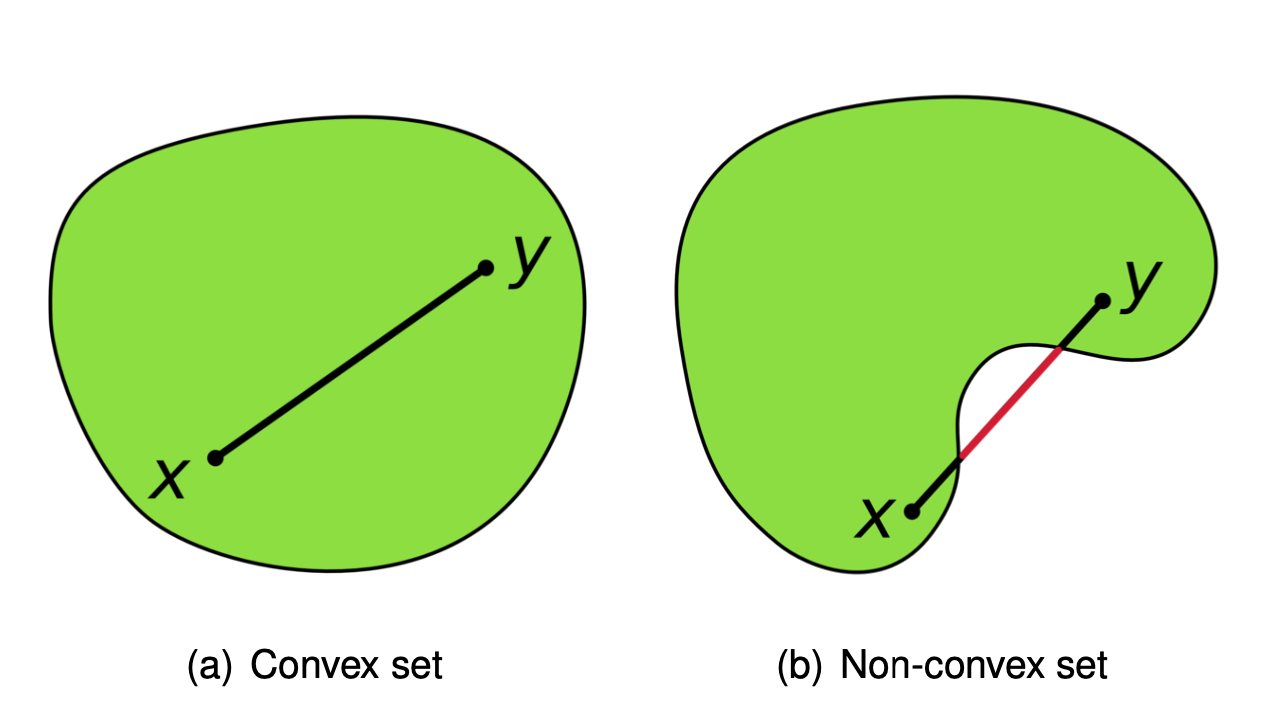
\includegraphics[scale=0.3]{Convex_set.png}
    \caption{Convex Set}
    \label{}
\end{figure}\end{center}

\begin{example}
Given $\vec{a}\in \mathbb{R}^n$ and $b\in \mathbb{R}$, the half spaces are convex
\begin{equation}
    \begin{aligned}
        \{\vec{x}\in \mathbb{R}^n: \vec{a}\vec{x}\geq b\}&\text{ (closed half-space)}\\
        \{\vec{x}\in \mathbb{R}^n: \vec{a}\vec{x}> b\}&\text{ (open half-space)}\\
    \end{aligned}
    \nonumber
\end{equation}
\end{example}

\begin{example}
$B(\vec{x},r)=\{\vec{y}\in \mathbb{R}^n:\|\vec{x}-\vec{y}\|< r\}$ is convex.
\end{example}

\subsubsection{Prop: convex sets $e_1,e_2,...e_n$, then $\cap_{i=1}^ne_i$ is convex}
\begin{proposition}
    If $C_1,C_2$ are convex sets, then $C_1\cap C_2$ is also convex.

    (Given a collection $e$ of convex sets, $\cap e$ is also convex)
\end{proposition}

\subsection{Convex Hull}
\begin{definition}[Convex Combinations]
A Convex Combination of $x_1,x_2,...,x_n\in \mathbb{R}^n$ is a linear combination $$\sum_{i=1}^k\lambda_ix_i\text{, such that }\sum_{i=1}^k\lambda_i=1,\lambda_i\geq 0,i=1,...,k$$
\end{definition}

\subsubsection{Convex Hull $conv(S)$ is the set of all convex combinations of points in $S$}
\begin{definition}[Convex Hull]
Given a set of points $S\subseteq \mathbb{R}^n$, the \textbf{convex hull} $conv(S)$ is the set of all convex combinations of points in $S$.

(Equivalencies: We can define the $conv(S)$ as the smallest convex set contains $S$)
\end{definition}

\subsubsection{Theorem: convex set $S$, convex combination $\lambda_1 x_1+\cdots+\lambda_k x_k\in S$, $\forall x_1,...,x_k\in S$}
\begin{theorem}
Consider a convex set $S$ and points $x_1,x_2,...,x_k\in S$, any convex combination $\lambda_1 x_1+\cdots+\lambda_k x_k$ is also in $S$
\end{theorem}
\begin{proof}
prove by induction. (Convex combination of any number points can be rewritten to a convex combination of two points.)
\end{proof}

\subsubsection{Corollary: $conv(S)$ is the smallest convex set containing $S$}
\begin{corollary}
    $conv(S)$ is the smallest convex set containing $S$.
\end{corollary}

\subsection{Optimization over Convex Set}
$$\min_{x\in \&} f(x)$$
where $\&$ is a non-empty closed and convex subset of $\mathbb{R}^n$.

Assume $f$ is continuously differentiable on $\&$.

\begin{definition}
$x^*$ is a \underline{local min of $f$ over $\&$} if $\exists \varepsilon>0$ s.t. $f(x^*)\leq f(x)\quad \forall x\in \&$ with $\|x-x^*\|<\varepsilon$.

$x^*$ is \underline{global min of $f$ over $\&$} if $f(x^*)\leq f(x)\quad \forall x\in \&$.
\end{definition}


\subsection{Convex Function}
\subsubsection{Definition: $f$ is convex $\Leftrightarrow$ $f(\alpha x+(1-\alpha) y) \leq \alpha f(x)+(1-\alpha) f(y), \forall x, y \in C, \forall \alpha \in[0,1]$}
\begin{center}
    \fcolorbox{black}{gray!10}{\parbox{.9\linewidth}{\underline{\textbf{Convex function} (0-th order)}: $f$ is \textbf{convex} in a convex set $C$ iff $f(\alpha x+(1-\alpha) y) \leq \alpha f(x)+(1-\alpha) f(y), \forall x, y \in C, \forall \alpha \in[0,1] .$ $f$ is \textbf{strictly convex} in a convex set $C$ iff $f(\alpha x+(1-\alpha) y) < \alpha f(x)+(1-\alpha) f(y), \forall x\neq y \in C, \forall \alpha \in[0,1] .$
    
    Alternative definitions of \underline{\textbf{convex function}} $f$:
    \begin{enumerate}[(1)]
        \item (differentiable): $f(z) \geq f(x)+(z-x)^{T} \nabla f(x), \ \forall x, z \in C .$
        \item (twice differentiable): $\nabla^{2} f(x) \succeq 0,\ \forall x \in C .$ ($C$ is open)
    \end{enumerate}
    }}
\end{center}

A function $f$ is a \underline{\textbf{concave function}} \underline{if and only if} $-f$ is a convex function.

\subsubsection{First-order: $f$ is convex $\Leftrightarrow$ $f(z) \geq f(x)+(z-x)^{T} \nabla f(x), \forall x, z \in C$}
\textbf{Alternative 1 ($1^{st}$ order)}: If $f$ is differentiable, then $f$ is convex \textbf{iff} $f(z) \geq f(x)+(z-x)^{T} \nabla f(x), \ \forall x, z \in C .$ The inequality is strict for strict convexity.
\begin{proof}
\quad
\begin{enumerate}[(i)]
    \item "$\Rightarrow$" \begin{equation}
        \begin{aligned}
            f(x+\alpha (y-x))&\leq (1-\alpha)f(x)+\alpha f(y), \forall \alpha \in (0,1)\\
            \Rightarrow	\frac{f(x+\alpha(y-x))-f(x)}{\alpha}&\leq f(y)-f(x)\\
            \text{Limit as }\alpha \rightarrow 0 \Rightarrow (y-x)^{T} \nabla f(x)&\leq f(y)-f(x)
        \end{aligned}
        \nonumber
    \end{equation}
    \item "$\Leftarrow$" Let $g=\alpha x+(1-\alpha) y$
    \begin{equation}
        \begin{aligned}
            f(g)+(x-g)^{T} \nabla f(g)&\leq f(x)\\
            f(g)+(y-g)^{T} \nabla f(g)&\leq f(y)\\
            \Rightarrow	f(g)&\leq \alpha f(x)+(1-\alpha)f(y)\\
            f(\alpha x+(1-\alpha) y)&\leq \alpha f(x)+(1-\alpha)f(y)
        \end{aligned}
        \nonumber
    \end{equation}
\end{enumerate}
\end{proof}

\subsubsection{Prop: local-min$\Rightarrow\nabla f(x^*)^T(x-x^*)\geq 0,\forall x\in \&$ $\Leftrightarrow$ global-min in convex }
\begin{proposition}[optimality conditions]
    \quad
    \begin{enumerate}[(a)]
        \item (Necessary Conditions for local-min) If $x^*$ is a local min of $f$ over $\&$, then $$\nabla f(x^*)^T(x-x^*)\geq 0\quad \forall x\in \&$$
        \item (Sufficient and Necessary Condition for global-min of convex $f$) If $f$ is convex over $\&$, then above condition is also sufficient for $x^*$ to be a global-min.
    \end{enumerate}
\end{proposition}
\begin{proof}
    \quad
\begin{enumerate}[(a)]
    \item Suppose $x^*$ is a local-min, and $\nabla f(x^*)^T(x-x^*)<0$ for some $x\in \&$.
    
    Let $g(\varepsilon)=f(x^*+\varepsilon(x-x^*))$, then $g'(\varepsilon)=\nabla f(x^*+\varepsilon(x-x^*))^T(x-x^*)$.
    
    By MVT(middle value theorem), $g(\varepsilon)=g(0)+\varepsilon g'(\beta\varepsilon)$ for some $\beta\in[0,1]$
    $$\Rightarrow f(x^*+\varepsilon(x-x^*))=f(x^*)+\varepsilon\nabla f(x^*+\beta\varepsilon(x-x^*))^T(x-x^*)\quad \text{for some }\beta\in[0,1]$$
    Since $\nabla f$ is continuous, we have that for all sufficient small $\varepsilon>0$, $\nabla f(x^*+\beta\varepsilon(x-x^*))^T(x-x^*)<0 \Rightarrow f(x^*+\varepsilon(x-x^*))=f(x^*)$

    Since $x^*+\varepsilon(x-x^*)=\varepsilon x+(1-\varepsilon)x^*\in \&$, then $x^*$ can't be a local-min over $\&$ $\rightarrow$ contradiction.
    \item Convexity of $f$ over $\&$ $\Rightarrow f(x)\geq f(x^*)+\nabla f(x^*)^T(x-x^*),\quad \forall x\in \&$.
    
    Thus,
    \begin{equation}
        \begin{aligned}
            &\nabla f(x^*)^T(x-x^*),\quad \forall x\in \&\\
            \Rightarrow	& f(x)\geq f(x^*)\quad \forall x\in \&\\
            \Rightarrow	& x^*\text{ is a global min of $f$ over }\&
        \end{aligned}
        \nonumber
    \end{equation}
\end{enumerate}
\end{proof}

\textbf{Example:}
\begin{align*}
    &\max_{x\in\&}\quad x_1^{a_1}x_2^{a_2}\cdots x_n^{a_n}\\
    &\begin{array}{r@{\quad}r@{}l@{\quad}l}
    &\&=\{x:\sum_{i=1}^nx_i=1,x_i\geq 0,i=1,2,...,n\} &\\
    &a_i,i=1,2,...,n \text{ are given positive scalars}&\\
\end{array} .
\end{align*}
Equivalent to $$\min_{x\in\&}\quad f(x)$$ with $f(x)=-\sum a_i\ln x_i$
\begin{equation}
    \begin{aligned}
        \nabla f(x)&=\left(-\frac{a_1}{x_1},-\frac{a_2}{x_2},...,-\frac{a_n}{x_n}\right)\\
        \nabla^2 f(x)&=diag\left(\frac{a_1}{x^2_1},\frac{a_2}{x^2_2},...,\frac{a_n}{x^2_n}\right)\succ 0\\
        &\Rightarrow f\text{ is strictly convex}.
    \end{aligned}
    \nonumber
\end{equation}
\begin{equation}
    \begin{aligned}
        x^*\in\&\text{ is (unique) min}&\Leftrightarrow \nabla f(x^*)^T(x-x^*)\geq 0\quad \forall x\in\&.\\
        &\Leftrightarrow -\sum_{i=1}^n\frac{a_i}{x_i^*}(x-x^*)\geq 0\quad \forall x\in\&.\\
        &\Leftrightarrow -\sum_{i=1}^na_i\frac{x_i}{x_i^*}+\sum_{i=1}^na_i\geq 0\quad \forall x\in\&.\\
    \end{aligned}
    \nonumber
\end{equation}
Guess: $x^*_i=\frac{a_i}{\sum_{i=1}^na_i}$. Then,
\begin{equation}
    \begin{aligned}
        -\sum_{i=1}^n a_i\frac{x_i}{x_i^*}+\sum_{i=1}^na_i=0,\quad \forall x\in\&
    \end{aligned}
    \nonumber
\end{equation}
Thus $x^*=\frac{a_i}{\sum_{i=1}^na_i}$ is unique min.


\subsubsection{Second-order: $f$ is convex $\Leftrightarrow$ $\nabla^{2} f(x) \succeq 0,\ \forall x \in C$}
\textbf{Alternative 2 ($2^{nd}$ order)}: If $f$ is twice differentiable and $C$ is open and convex, then $f$ is convex iff
$$
\nabla^{2} f(x) \succeq 0,\ \forall x \in C
$$
\begin{proof}
    \begin{enumerate}
        \item[$\Rightarrow$]: Suppose $f:C \rightarrow \mathbb{R}$ is convex and take $x^*\in C$. Define $g: C \rightarrow \mathbb{R}$ as $g(y)=f(y)-(y-x^*)\nabla f(x^*)$. Because $g$ is a sum of convex functions ($f(y)$ and $-(y-x^*)\nabla f(x^*)$ which is linear), $g$ is convex.
        
        Because $\nabla g(y)=\nabla f(y)-\nabla f(x^*)$, $x^*$ is the critical point of $g$, $x^*$ is the global min of $g$. We can also show $Hg(y)=Hf(y)$. If $Hg(x^*)=Hf(x^*)$ is not positive semidefinite, then we had a negative eigenvalue $u$ s.t. $g(x^*+tu)$ is decreasing in $t$ s.t. $x^*$ is not a global minimizer of $g$, contradiction. Since $x^*$ is arbitrary, $Hg(x^*)\succeq 0,\forall x^*\in C$.
        \item[$\Leftarrow$]: \textbf{Taylor:} Given a function $f:\mathbb{R}^n \rightarrow \mathbb{R}$, if $Hf$ is continuous and $\vec{x}^*$ is a critical point of $f$, then
        $$f(\vec{x})=f(\vec{x}^*)+\nabla f(\vec{x}^*)(\vec{x}-\vec{x}^*)+\frac{1}{2}(\vec{x}-\vec{x}^*)^T Hf(\vec{z}) (\vec{x}-\vec{x}^*)$$
        for some $\vec{z}$ on the line between $\vec{x}$ and $\vec{x}^*$.
    \end{enumerate}
\end{proof}





\subsubsection{Sufficient Condition of Strictly Convex: $\nabla^{2} f(x) \succ 0$}
Strictly convex: $\nabla^{2} f(x) \succ 0,\ \forall x \in C \text{ ($C$ is open)} \Rightarrow	$ $f$ is strictly convex.


\textbf{Note:} $f$ is strictly convex $\nRightarrow \nabla^{2} f(x) \succ 0$.
\begin{example}
$f(x)=x^4\text{(strictly convex)}$, $\frac{d^2f(x)}{dx^2}=12x^2(=0\text{ at }x=0)$
\end{example}


\subsubsection{Prop: Max and Linear combination of convex functions are also convex}
\textbf{Properties: }Convex functions $f$ over $\mathbb{R}^n$, $\{f_i\}_{i\in \mathbb{Z}}$ over $\&$:
\begin{enumerate}[(1)]
    \item $C=\{x\in \mathbb{R}^n| f(x)\leq a\}$ is convex set, $\forall a\in \mathbb{R}$.
    \item Suppose $\{f_i\}_{i\in \mathbb{Z}}$ are convex functions $C \rightarrow \mathbb{R}$. $\alpha_1,\alpha_2,...,\alpha_k$ are positive scalars, then $$f_{sum}(x)=\sum_{i=1}^k\alpha_if_i(x)$$ is convex. If at least on $f_i$ is strictly convex, $f_{sum}$ is strictly convex.
    \item $f_{max}(x)=\max_{i=1,...,k}f_i(x)$ is convex over $\&$ (strictly convex if all $f_i$ are strictly convex)
\end{enumerate}
\begin{proof} Prove (2) here:\\
    We need to show (1) $\alpha f_i$ is convex; (2) $H(x)=f_1(x)+f_2(x)$ is convex and strictly convex if one is strictly convex.

    (1): can be proved by definition.\\
    (2): $H(\lambda x+(1-\lambda)y)=f_1(\lambda x+(1-\lambda)y)+f_2(\lambda x+(1-\lambda)y)\leq \lambda (f_1(x)+f_2(x))+(1-\lambda)(f_1(y)+f_2(y))=\lambda H(x)+(1-\lambda)H(y),\lambda\in [0,1]$ $\Rightarrow$ $H$ is convex. (We can get strict inequality if one is strictly convex).
\end{proof}
\begin{proof} Prove (3) here:
\begin{equation}
    \begin{aligned}
        f_{max}(\alpha x+(1-\alpha)y)&=\max_{i=1,...,k}f_i(\alpha x+(1-\alpha)y)\\
    &\leq \max_{i=1,...,k}[\alpha f_i(x)+(1-\alpha)f_i(y)]\\
    &\leq \max_{i=1,...,k}\alpha f_i(x)+\max_{i=1,...,k}(1-\alpha)f_i(y)\\
    &=\alpha f_{max}(x)+(1-\alpha)f_{max}(y)
    \end{aligned}
    \nonumber
\end{equation}
Inequality is strict if all $f_i$ are strictly convex.
\end{proof}



\subsection{Lemma: function $f$ is a convex function iff $\phi(t)=f(\vec{x}+t\vec{u})$ is convex of $t$}
\begin{lemma}
    Let $C\subseteq \mathbb{R}^n$ be a convex set. A function $C \rightarrow \mathbb{R}$ is convex if and only if, for all $\vec{x}\in C$ and $\vec{u}\in \mathbb{R}^n$, the function $$\phi(t)=f(\vec{x}+t\vec{u})$$ is a single-variable convex function of $t$.
\end{lemma}

\subsection{Proposition: Convex function $f$, $\nabla f(x^*)=0$ $\Rightarrow$ global-min}
\begin{proposition}
    Let $f: X \longmapsto \mathbb{R}$ be a convex function over the convex set $X$.

    (a) A local-min of $f$ over $X$ is also a global-min over $X$. If $f$ is strictly convex, then min is unique.

    (b) If $X$ is open (e.g. $\mathbb{R}^{n}$ ), then $\nabla f\left(x^{*}\right)=0$ is a necessary and sufficient condition for $x^{*}$ to be a global minimum.
\end{proposition}
\begin{proof}
\quad\\
Proof based on a property: If $f$ is differentiable over $C$ (open), then $f$ is convex iff
$$
f(z) \geq f(x)+(z-x)^{\prime} \nabla f(x), \quad \forall x, z \in C .
$$
\end{proof}


\begin{corollary}
    Let $f: X \longmapsto \mathbb{R}$ be a concave function over the convex set $X$.

    (a) A local-max of $f$ over $X$ is also a global-max over $X$.

    (b) If $X$ is open (e.g. $\mathbb{R}^{n}$ ), then $\nabla f\left(x^{*}\right)=0$ is a necessary and sufficient condition for $x^{*}$ to be a global maximum.
\end{corollary}





\subsection{Application: Unconstrained Quadratic Optimization}
$$\begin{array}{ll}\text { minimize } & f(\mathbf{w})=\frac{1}{2} \mathbf{w}^{T} \mathbf{Q} \mathbf{w}-\mathbf{b}^{T} \mathbf{w} \\ \text { subject to } & \mathbf{w} \in \mathbb{R}^{d}\end{array}$$
where $\mathbf{Q}$ is a symmetric $d \times d$ matrix. (what if non-symmetric?)
$$\nabla f(\mathbf{w})=\mathbf{Q}\mathbf{w}-\mathbf{b},\ \nabla^2 f(\mathbf{w})=\mathbf{Q}$$
\begin{enumerate}[(i)]
    \item $\mathbf{Q}\succeq 0 \Leftrightarrow	f$ is convex.
    \item $\mathbf{Q}\succ 0 \Leftrightarrow	f$ is strictly convex.
    \item $\mathbf{Q}\preceq 0 \Leftrightarrow	f$ is concave.
    \item $\mathbf{Q}\prec 0 \Leftrightarrow	f$ is strictly concave.
\end{enumerate}









- Necessary condition for (local) optimality
$$
\mathbf{Q} \mathbf{w}=\mathbf{b}, \quad \mathbf{Q} \succeq 0
$$

Case 1: $\mathbf{Q w}=\mathbf{b}$ has no solution, i.e. $\mathbf{b} \notin R(\mathbf{Q})$. No stationary point, no lower bound ($f$ can achieve $-\infty$).

Case 2: $\mathbf{Q}$ is not PSD ( $f$ is non-convex)
No local-min, no lower bound ($f$ can achieve $-\infty$).

Case 3: $\mathbf{Q} \succeq 0$ (PSD) and $\mathbf{b} \in R(\mathbf{Q})$. Convex, has global-min, 
any stationary point is a global optimal solution.

\begin{example}
    Toy Problem 1: $\min _{x, y \in \mathbb{R}} f(x, y) \triangleq x^{2}+y^{2}+\alpha x y$.
\end{example}
\begin{enumerate}
    \item Step 1: First order condition: $2 x^{*}+\alpha y^{*}=0,2 y^{*}+\alpha x^{*}=0$.
    
    - We get $4 x^{*}=-2 \alpha y^{*}=\alpha^{2} x^{*}$. So $\left(4-\alpha^{2}\right) x^{*}=0$.
    
    - Case 1: $\alpha^{2}=4$. If $x^{*}=-\alpha y^{*} / 2$, then $\left(x^{*}, y^{*}\right)$ is a stationary point.
    
    - Case 2: $\alpha^{2} \neq 4$. Then $x^{*}=0 ; y^{*}=-\alpha x^{*} / 2=0$. So $(0,0)$ is stat-pt.
    \item Step 2: Check convexity. Hessian $\nabla^{2} f(x, y)=\left(\begin{array}{ll}2 & \alpha \\ \alpha & 2\end{array}\right)$.
    
    Eigenvalues $\lambda_{1}, \lambda_{2}$ satisfy $\left(\lambda_{i}-2\right)^{2}=\alpha^{2}, i=1,2$.
    Thus $\lambda_{1,2}=2 \pm|\alpha|$.

    - If $|\alpha| \leq 2$, then $\lambda_{i} \geq 0, \forall i$. Thus $f$ is convex. Any stat-pt is global-min.

    - If $|\alpha|>2$, at least one $\lambda_{i}<0$, thus $f$ is not convex.
    \item Step 3 (can be skipped now): For non-convex case $(|\alpha|>2)$, prove no lower bound.
    
    $f(x, y)=(x+\alpha y / 2)+\left(1-\alpha^{2} / 4\right) y^{2}$. Pick $y=M, x=-\alpha M / 2$, then
    $f(x, y)=\left(1-\alpha^{2} / 4\right) M^{2} \rightarrow-\infty$ as $M \rightarrow \infty$.
\end{enumerate}

Summary:

If $|\alpha|>2$, no global-min, $(0,0)$ is stat-pt;

if $|\alpha|=2$, any $(-0.5 \alpha t, t), t \in \mathbb{R}$ is a stat-pt and global-min;

if $|\alpha|<2,(0,0)$ is the unique stat-pt and global-min.

\begin{example}
Linear Regression
\end{example}
$\text{minimize } f(\mathbf{w})=\frac{1}{2}\left\|\vec{x}^{T} \mathbf{w}-\vec{y}\right\|^{2}$ subject to $ \mathbf{w} \in \mathbb{R}^{d}$

$n$ data points, $d$ features

- $\vec{x}$ may be wide (under-determined), tall (over-determined), or rank-deficient

- Note that comparing with the previous case, $\mathbf{Q}=\mathbf{X X}^{T} \in \mathbb{R}^{d \times d}$, $\mathbf{b}=\vec{x} \vec{y} \in \mathbb{R}^{d \times 1}$

- $\mathbf{Q} \succeq 0$; Case 2 never happens!

- First order condition $\mathbf{X X}^{\top} \mathbf{w}^{*}=\vec{x} \vec{y}$.

\quad - It always has a solution; Case 1 never happens!

\begin{claim}
    Linear regression problem is always convex; it has global-min.
\end{claim}
\textbf{Claim}
$$
\mathbf{X X}^{\top} \mathbf{w}^{*}=\vec{x} \vec{y}
$$
which always has a solution.

If $X X^{\top} \in \mathbb{R}^{d \times d}$ is invertible (only happen when $n \geq d$ ), then there is a unique stationary point $x=\left(A^{\top} A\right)^{-1} A^{\top} b$. It is also a global minimum.

If $X X^{\top} \in \mathbb{R}^{d \times d}$ is not invertible, then there can be infinitely many stationary points, which are the solutions to the linear equation.
All of them are global minima, giving the same function value.



\subsection{Theorem: If $f$ is convex and $g$ is convex and increasing, $(g\cdot f)(x)$ is convex}
\begin{theorem}
    If $f$ is convex and $g$ is convex and increasing, $(g\cdot f)(x)=g(f(x))$ is convex. Moreover, if $f$ is strictly convex and $g$ is strictly increasing $g\cdot f$ is strictly convex.
\end{theorem}
\begin{proof}
$g(f(\lambda x+(1-\lambda)y))\leq g(\lambda f(x)+(1-\lambda) f(y))\leq \lambda g(f(x))+(1-\lambda)g(f(y))$ (the first inequality is strict when $f$ is strictly convex and $g$ is strictly increasing)
\end{proof}
\begin{corollary}
    $f(x)=|x|^p,p\geq 1$ is convex. ($f_1(x)=|x|$ is convex in $\mathbb{R}$, $f_2(x)=x^p,p\geq 1$ is convex in $\mathbb{R}^+\cup\{0\}$)
\end{corollary}
Except proving $f(x)=|x|^p,p\geq 1$ is convex we can also prove $f(x)=|x|^p,p\in(1,2]$ is strongly convex in $[-1,1]$.
\begin{corollary}
    $f(x)=|x|^p,p\in(1,2]$ is strongly convex in $[-1,1]$.
\end{corollary}
\begin{proof}
$F(x)=f(x)-mx^2=|x|^p-\frac{m}{2}x^2$. $g_1(x)=|x|,x\in [-1,1]$ is convex; We want to prove $g_2(x)=x^p-\frac{m}{2}x^2,x\in [0,1]$ is also convex:
\begin{enumerate}[(1)]
    \item $p= 2$ ($g_2$ is twice differentiable): $g_2^{''}(x)=p(p-1)-m\geq 0$ for $m\leq p(p-1)$ $\Rightarrow$ $g_2(x)$ is convex and increasing in $[0,1]$.
    \item $p\in (1,2)$ ($g_2$ is not twice differentiable at $0$): $g_2^{'}(x)=px^{p-1}-mx$. Let
    \begin{equation}
        \begin{aligned}
            G_x(y)&=g_2(y)+(x-y)g_2^{'}(y),\ y\in [0,1]\\
            \frac{\partial G_x(y)}{\partial y}&=xg^{''}_2(y)-yg^{''}_2(y)=(x-y)g^{''}_2(y)\\
            &=\left(p(p-1)y^{p-2}-m\right)(x-y),\ y\in(0,1]
        \end{aligned}
        \nonumber
    \end{equation}
    for $m\leq p(p-1)$, $\frac{\partial G_x(y)}{\partial y}\geq 0, y\in (0,x]$ and $\frac{\partial G_x(y)}{\partial y}\leq 0, y\in [x,1]$.

    Then $G_x(y)\leq G_x(x),\forall y\in (0,1]$

    $G_x(0)=0$, $G_x(x)=g_2(x)=x^p-\frac{m}{2}x^2$. Since we know $g_2(x)\geq 0,\forall x\in [0,1]$ if $m\leq 2$, we can infer $G_x(y)\leq g_2(x)$. i.e., $g_2(y)+(x-y)g_2^{'}(y)\leq g_2(x),\forall x,y\in [0,1]$. Then we can infer $g_2(x)$ is convex and increasing for $m<p(p-1)$.
\end{enumerate}
\end{proof}

\subsection{Corollary: $f$ is linear, $g$ is convex (not necessarily increasing) $\Rightarrow$ $g\cdot f$ is convex}
\begin{corollary}
    Suppose $f:\mathbb{R}^m \rightarrow \mathbb{R}^n$ with $f(x)=Ax+b$ and $g:C \rightarrow \mathbb{R}$ is convex, then $h(x)=g(f(x))$ is convex as function $f^{-1}(C) \rightarrow \mathbb{R}$.
\end{corollary}
\begin{proof}
For $\lambda\in[0,1]$,
\begin{equation}
    \begin{aligned}
        h(\lambda x+(1-\lambda)y)&=g(f(\lambda x+(1-\lambda)y))= g(\lambda(Ax+b)+(1-\lambda)(Ay+b))\\
        &\leq \lambda g(Ax+b)+(1-\lambda)g(Ay+b)=\lambda h(x)+(1-\lambda)h(y)
    \end{aligned}
    \nonumber
\end{equation}
\end{proof}


\begin{example}
    Prove $f(x,y,z)=(\frac{x}{2})^x(\frac{y}{3})^y(\frac{z}{4})^z$ is convex on $\{x>0,y>0,z>0\}$
\end{example}
We can rewrite the function
\begin{equation}
    \begin{aligned}
        f(x,y,z)=e^{x\ln(\frac{x}{2})+y\ln(\frac{y}{3})+z\ln(\frac{z}{4})}=g(h(x,y,z))
    \end{aligned}
    \nonumber
\end{equation}
where $h(x,y,z)=x\ln(\frac{x}{2})+y\ln(\frac{y}{3})+z\ln(\frac{z}{4})$ and $g(x)=e^x$.

$\frac{\partial^2 x\ln(\frac{x}{c})}{\partial x^2}=\frac{1}{x}>0$ $\Rightarrow$ $h(x,y,z)$ is convex. And we can check $g(x)$ si convex and increasing. We can know $f(x,y,z)$ is convex.

\subsection{Epigraph and Jensen's Inequality}
\subsubsection{Def: epigraph ${epi}(f)=\{(x,y)\in C\times \mathbb{R}:y\geq f(x)\}$}
\begin{definition}
    Given a subset $C \subseteq \mathbb{R}^n$ and a function $f: C \rightarrow \mathbb{R}$, the \textbf{epigraph} of $f$ is a set $${epi}(f)=\{(x,y)\in C\times \mathbb{R}:y\geq f(x)\}$$
\end{definition}

\subsubsection{Lemma: $f$ is convex function $\Leftrightarrow$ ${epi}(f)$ is a convex set}
\begin{lemma}
    Consider some $f: C \rightarrow \mathbb{R}$ where $C\subseteq \mathbb{R}^n$ is a convex set. Then $f$ is a convex function \textbf{iff} ${epi}(f)$ is a convex set.
\end{lemma}
\begin{proof}
Prove $\Rightarrow$: Suppose $f$ is a convex set and for any points in $epi(f)$, $(x_1,y_1),(x_2,y_2)\in epi(f)$.
\begin{equation}
    \begin{aligned}
        \lambda y_1+(1-\lambda)y_2\geq \lambda_1f(x_1)+(1-\lambda)f(x_2)\geq f(\lambda x_1+(1-\lambda)x_2)
    \end{aligned}
    \nonumber
\end{equation}
($\lambda\in[0,1]$)
By definition $\Rightarrow$ $\lambda y_1+(1-\lambda)y_2$ is also in ${epi}(f)$ $\Rightarrow$ ${epi}(f)$ is a convex set.

Prove $\Leftarrow$: Suppose ${epi}(f)$ is a convex set. For $x_1,x_2\in C$, by definition $(x_1,f(x_1)),(x_2,f(x_2))\in {epi}(f)$. Then $(\lambda x_1+(1-\lambda)x_2,\lambda f(x_1)+(1-\lambda)f(x_2))\in {epi}(f)$ $\Rightarrow$ $\lambda f(x_1)+(1-\lambda)f(x_2))\geq f(\lambda x_1+(1-\lambda)x_2)$ $\Rightarrow$ $f$ is convex.
\end{proof}

\subsubsection{Jensen's Inequality: $f(\sum_{i=1}^k\lambda_i x_i)\leq \sum_{i=1}^k\lambda_if(x_i)$}
\begin{theorem}[Jensen's Inequality]
    For any $\lambda_i\geq 0,i=1,...,k$ and $\sum_{i=1}^k\lambda_i=1$, if $f: C \rightarrow \mathbb{R}$ is convex and $\{x_i,i=1,...,k\}$ is a collection of points in $C$, then $$f(\sum_{i=1}^k\lambda_i x_i)\leq \sum_{i=1}^k\lambda_if(x_i)$$
\end{theorem}

Note: If $f$ is strictly convex and $\lambda_i>0,\forall i$, then $f(\sum_{i=1}^k\lambda_i x_i)= \sum_{i=1}^k\lambda_if(x_i)$ iff $x_1=x_2=\cdots=x_k$.
\begin{proof}
    For each $\vec{x}_1,...,\vec{x}_k$, there is a corresponding point $(\vec{x}_1,f(\vec{x}_1)),(\vec{x}_2,f(\vec{x}_2)),...,(\vec{x}_k,f(\vec{x}_k))\in {epi}(f)$. Because ${epi}(f)$ is convex,
    \begin{equation}
        \begin{aligned}
            \lambda_1 \begin{bmatrix}
                \vec{x}_1\\
                f(\vec{x}_1)
            \end{bmatrix}+\cdots+\lambda_k \begin{bmatrix}
                \vec{x}_k\\
                f(\vec{x}_k)
            \end{bmatrix}\in {epi}(f)
        \end{aligned}
        \nonumber
    \end{equation}
    i.e. $\begin{bmatrix}
        \lambda_1\vec{x}_1+\cdots+\lambda_k\vec{x}_k\\
        \lambda_1f(\vec{x}_1)+\cdots+\lambda_kf(\vec{x}_k)
    \end{bmatrix}\in{epi}(f)$. This means that $$\lambda_1f(\vec{x}_1)+\cdots+\lambda_k f(\vec{x}_k)\geq f(\lambda_1\vec{x}_1+\cdots+\lambda_k\vec{x}_k)$$
\end{proof}

\subsection{ Subgradients of Convex Functions}
Consider convex functions that are unlikely to be differentiable everywhere.
\subsubsection{Sub-gradient $\vec{d}$: $f(\vec{x})\geq f(\vec{x}^*)+\vec{d}\cdot (\vec{x}-\vec{x}^*), \forall \vec{x}\in C$}
\begin{lemma}
    If $C\subseteq \mathbb{R}^n$ is a convex set, $f: C \rightarrow  \mathbb{R}$ is a convex function, and $\vec{x}^*\in int(C)$, then there exists some vector $\vec{d}\in \mathbb{R}^n$ such that $$f(\vec{x})\geq f(\vec{x}^*)+\vec{d}\cdot (\vec{x}-\vec{x}^*),\ \forall \vec{x}\in C$$
\end{lemma}
\begin{definition}
    The $\vec{d}$ satisfied the inequality is called a \textbf{sub-gradient} of $f$ at $\vec{x}^*$.
\end{definition}
\begin{proof}
    We can use epigraphs. Recall that for a function $f: C \rightarrow \mathbb{R}$, $$epi(f)=\{(\vec{x},y)\in \mathbb{R}^{n+1}: y\geq f(\vec{x})\}$$
    when $C$ is a convex set and $f$ is a convex function, $epi(f)$ is a convex set.\\
    Choose $\vec{x}^*\in int(C)$, then $\left(\vec{x}^*,f(\vec{x}^*)\right)$ is a boundary point of $epi(f)$.\\
    By the support theorem, there exists a vector $(\vec{a},b)\in \mathbb{R}^{n+1}$ with $\|(\vec{a},b)\|=1$ such that
    \begin{equation}
        \begin{aligned}
            (\vec{a},b)\cdot \left(\vec{x}^*,f(\vec{x}^*)\right)&\geq (\vec{a},b)\cdot \left(\vec{x},y\right)\\
            \vec{a}\cdot \vec{x}^*+ b f(\vec{x}^*)&\geq \vec{a}\cdot \vec{x}+ by,\ \forall \left(\vec{x},y\right)\in epi(f)
        \end{aligned}
        \nonumber
    \end{equation}
    Specifically, we substitute $(\vec{x}^*,f(\vec{x}^*)+\varepsilon)\in epi(f)$ into the inequality, where $\varepsilon\geq 0$, $b\varepsilon\leq 0$ $\Rightarrow b\leq 0$.\\
    If $b=0$, $\vec{a}\cdot \vec{x}^*\geq \vec{a}\cdot \vec{x},\forall \vec{x}\in C$. By the separation theorem and $\vec{x}^*\in int(C)$, we can there must exist $\vec{y}\in C$ such that $\vec{a}\cdot \vec{y}>\vec{a}\cdot \vec{x}^*$ which contradicts to the inference. Hence, $b>0$.\\
    Substitute the form $(\vec{x},f(\vec{x}))$,
    \begin{equation}
        \begin{aligned}
            \vec{a}\cdot \vec{x}^*+ b f(\vec{x}^*)&\geq \vec{a}\cdot \vec{x}+ bf(\vec{x})\\
            bf(\vec{x})&\leq bf(\vec{x}^*)-\vec{a}(\vec{x}-\vec{x}^*)
        \end{aligned}
        \nonumber
    \end{equation}
    Since $b<0$, we can divide the equation by $b$ on each side:
    \begin{equation}
        \begin{aligned}
            f(\vec{x})&\geq f(\vec{x}^*)-\frac{\vec{a}}{b}(\vec{x}-\vec{x}^*)
        \end{aligned}
        \nonumber
    \end{equation}
    The set of all available $-\frac{\vec{a}}{b}$ are the sub-gradient we want.
\end{proof}
\subsubsection*{\underline{Properties of Sub-gradient}}
\begin{enumerate}[1)]
    \item Sub-gradient always exist at any point for convex functions.
    \item If $\nabla f$ exists at a point $x$ for convex $f$ $\Leftrightarrow$ Sub-gradient is \underline{unique and $=\nabla f(x)$}
    \item Some definition for sub-gradient can be applied for non-convex $f$, but sub-gradient may not exist.
\end{enumerate}

\begin{example}
$f(x)=|x|,x\in \mathbb{R}$
\end{example}
For $x\neq 0$, $\nabla f$ exists and $=$ sub-gradient.\\
For $x=0$, any $g\in[-1,1]$ is a sub-gradient.
\begin{proof}\quad
\begin{enumerate}[(1)]
    \item For $y>0$, $f(y)=y\geq f(0)+gy=gy,\forall g\in[-1,1]$
    \item For $y<0$, $f(y)=-y\geq f(0)+gy=gy,\forall g\in[-1,1]$
\end{enumerate}
\end{proof}

\subsubsection{Sub-differential: set of all sub-gradient}
\begin{definition}
    Set of all sub-gradient of $f$ at $\vec{x}^*$ is called \textbf{sub-differential} of $f$ at $\vec{x}^*$, denoted $\partial f(\vec{x}^*)$.
\end{definition}
\begin{example}
For $f(x)=|x|$,
\begin{equation}
    \begin{aligned}
        \partial f(x)=\left\{\begin{matrix}
            -1&\text{ if }x<0\\
            [-1,1]&\text{ if }x=0\\
            1&\text{ if }x>0\\
        \end{matrix}\right.
    \end{aligned}
    \nonumber
\end{equation}
\end{example}

\begin{example}
For $f(x)=\max\{1,|x|-1\}$. (Note: $f(x)$ is convex since $1,|x|-1$ are both convex.)
\begin{equation}
    \begin{aligned}
        \partial f(x)=\left\{\begin{matrix}
            -1&\text{ if }x<-2\\
            [-1,0]&\text{ if }x=-2\\
            0&\text{ if }-1<x<2\\
            [0,1]&\text{ if }x=2\\
            1&\text{ if }x>2\\
        \end{matrix}\right.
    \end{aligned}
    \nonumber
\end{equation}
\end{example}
When $x=2$,
\begin{equation}
    \begin{aligned}
        f(y)=\max\{1,|y|-1\}\geq f(2)+g(y-2)=1+g(y-2)
    \end{aligned}
    \nonumber
\end{equation}
\begin{enumerate}[(1)]
    \item \underline{$y\geq 0$}: $0\geq g(y-2)$ or $0\geq (g-1)(y-2)$. If $y>2$, $g\leq 1$; If $y=2$, $\forall g$; If $0\leq y< 2$, $g\geq 0$. $\Rightarrow g\in[0,1]$
    \item \underline{$y< 0$}: $0\geq g(y-2)$ or $-y-2\geq g(y-2)$, i.e. $g\geq 0$ or $g\leq \frac{2+y}{2-y}$ (satisfied by $g\in[0,1]$)
\end{enumerate}

\subsubsection{More examples}
\begin{example}
    $f(x)=-\sqrt{x},\ x\in C=[0,\infty)$
\end{example}
It does not have a sub-gradient at $x^* = 0$, because the only possible tangent line is vertical. This shows that the hypothesis $x^*\in int(C)$ is necessary.




\begin{example}
    $f(x)=\|x\|=\sqrt{x^Tx}$
\end{example}
\begin{enumerate}[$\bullet$]
    \item $f$ is convex (by Triangle Inequality: $\|x\|+\|y\|\geq \|x+y\|$)
    \item For $x\neq 0$, $\nabla f(x)$ exists and $$\partial f(x)= \nabla f(x) =\frac{1}{2\sqrt{x^Tx}}\cdot 2x=\frac{x}{\|x\|}$$
    \item If $x=0$, $\nabla f(x)$ doesn't exist.\\
    \textbf{Claim:} $\partial f(0)=\{g\in \mathbb{R}^n:\|g\|\leq 1\}$
    \begin{proof}
        Need to show that for $\|g\|\leq 1$ and $\forall y\in \mathbb{R}^n$, $$f(y)=\|y\|\geq f(0)+g^T(y-0)=g^T y$$
        But by Cauchy-Schwarz inequality, for $\|g\|\leq 1$, $$g^Ty\leq \|g\|\|y\|\leq \|y\|,\forall y\in \mathbb{R}^n$$
        To estabilish the converse, suppose $\|g\|>1$.

        Then, setting $y=\frac{g}{\|g\|}$ $\Rightarrow$ $\|y\|=1$ but $g^Ty=\|g\|>1=\|y\|$
    \end{proof}
\end{enumerate}

\begin{example}
    $f(x)=|x_1-x_2|\leftarrow$ convex
\end{example}
\begin{enumerate}[$\bullet$]
    \item If $x_1>x_2$, $|x_1-x_2|=x_1-x_2$, and $\nabla f$ exists and $(1,-1)$
    \item If $x_1<x_2$, $|x_1-x_2|=x_2-x_1$, and $\nabla f$ exists and $(-1,1)$
    \item \textbf{Claim:} If $x_1=x_2$, $\partial f(x)=\{(a,b):a=-b,|a|\leq 1\}$
    \begin{proof}
        Suppose $x_1=x_2=c$. Then we need to show $\forall y\in \mathbb{R}^2$, $(a,b)$ s.t. $a=-b$, $|a|\leq 1$
        \begin{equation}
            \begin{aligned}
                |y_1-y_2|\geq f(c,c)+[a\ b]\begin{bmatrix}
                    y_1-c\\
                    y_2-c
                \end{bmatrix}=ay_1+by_2-c(a+b)=a(y_1-y_2)
            \end{aligned}
            \nonumber
        \end{equation}
        Since $|a|<1$, this inequality holds $\forall y\in \mathbb{R}^2$
        
        To show the converse,
        \begin{enumerate}
            \item Suppose $a\neq -b$.
            
            If $c(a+b)<0$, setting $y_1=y_2=0$. $\Rightarrow |y_1-y_2|=0$, and $ay_1+by_2-c(a+b)=-c(a+b)>0=|y_1-y_2|$, above inequality fails to hold.
    
            If $c(a+b)>0$, setting $y_1=y_2=2c$. $\Rightarrow |y_1-y_2|=0$, and $ay_1+by_2-c(a+b)=c(a+b)>0=|y_1-y_2|$, above inequality fails to hold.
    
            If $c=0$, setting $y_1=y_2=(a+b)$. $\Rightarrow |y_1-y_2|=0$, and $ay_1+by_2-c(a+b)=(a+b)^2>0=|y_1-y_2|$, above inequality fails to hold.
            \item Suppose $a=-b$ with $|a|>1$.
            
            If $a>1$, setting $y_1=y_2+1$; If $a<-1$, setting $y_1=y_2-1$.
    
        \end{enumerate}
    \end{proof}
\end{enumerate}
























\section{Geometric Programming (GP)}

\subsection{Arithmetic Mean-Geometric Mean Inequality (A-G inequality) $\delta_1x_2+\delta_2x_2+\cdots+\delta_nx_n\geq x_1^{\delta_1}x_2^{\delta_2}\cdots x_n^{\delta_n}$}
\begin{theorem}[A-G inequality]
For any $x_1,x_2,..,x_n\geq 0$, $$\frac{x_1+x_2+\cdots+x_n}{n}\geq \sqrt[n]{x_1x_2\cdots x_n}$$
Equality is only achieved when $x_1=x_2=\cdots=x_n$
\end{theorem}
\begin{enumerate}[$\bullet$]
    \item The LHS is the arithmetic mean (average) of $x_1,x_2,...,x_n$.
    \item The RHS is the geometric mean of $x_1,x_2,...,x_n$.
\end{enumerate}

\begin{theorem}[Weighted A-G inequality]
    For any $x_1,x_2,...,x_n\geq 0$ with $\lambda_1,\lambda_2,\cdots,\lambda_n>0$ with $\delta_1+\cdots+\delta_n=1$, $$\delta_1x_2+\delta_2x_2+\cdots+\delta_nx_n\geq x_1^{\delta_1}x_2^{\delta_2}\cdots x_n^{\delta_n}$$
    Equality is only achieved if $x_1=x_2=\cdots=x_n$.
\end{theorem}
When $\delta_1=\cdots=\delta_n=\frac{1}{n}$, the inequality recovers to unweighted A-G inequality.
\begin{proof}Prove by Jensen's Inequality:\\
    Let $f(t)=-\ln(t)$ which is strictly convex in $(0,\infty)$. Take $\lambda_1,\lambda_2,\cdots,\lambda_n>$ such that $\delta_1+\delta_2+\cdots+\delta_n=1$. According to Jensen's Inequality: $$f(\sum_{i=1}^n\delta_i x_i)\leq \sum_{i=1}^n\delta_i f(x_i)$$
    By substituting $f$:
    \begin{equation}
        \begin{aligned}
            -\ln(\sum_{i=1}^n\delta_i x_i)&\leq -\sum_{i=1}^n\delta_i \ln(x_i)\\
            e^{\ln(\sum_{i=1}^n\delta_i x_i)}&\geq e^{\sum_{i=1}^n\delta_i \ln(x_i)}\\
            \sum_{i=1}^n\delta_i x_i&\geq x_1^{\delta_1}x_2^{\delta_2}\cdots x_n^{\delta_n}
        \end{aligned}
        \nonumber
    \end{equation}
\end{proof}

\subsection{Unconstrained Geometric Programs}
\subsubsection{Def: Posynomial}
\begin{definition}
    A \textbf{posynomial term} in variables $t_1,...,t_m$ is a function of the form $$Ct_1^{\alpha_1}t_2^{\alpha_2}\cdots t_m^{\alpha_m}$$ where $\alpha_1,...,\alpha_m\in \mathbb{R}$ and $C>0$ is a positive real number.
\end{definition}
\begin{definition}
    A \textbf{posynomial} is a sum of posynomial terms.
\end{definition}

\subsubsection{General Strategy: A-G inequality}
\begin{definition}
    An unconstrained geometric program (GP) is the problem of minimizing a posynomial over positive real inputs.
    $$\min_{(t_1,\cdots,t_m\in \mathbb{R}^m_{>0}}g(t_1,\cdots,t_m)$$
    where $g(t_1,\cdots,t_m)$ is a sum of posynomial terms. $g(t_1,\cdots,t_m)=\sum_{i=1}^n{Term}_i(t_1,\cdots,t_m)$, where ${Term}_i(t_1,\cdots,t_m)=C_i t_1^{\alpha_{i,1}}t_2^{\alpha_{i,2}}\cdots t_m^{\alpha_{i,m}}$
\end{definition}

\begin{center}
    \fcolorbox{black}{gray!10}{\parbox{.9\linewidth}{\textbf{General Strategy:}\\
    Choose weights $\delta_1,...,\delta_n>0$ with $\delta_1+\cdots+\delta_n=1$ and use the inequality
    \begin{equation}
        \begin{aligned}
            \sum_{i=1}^n{Term}_i(t_1,\cdots,t_m)&=\sum_{i=1}^n\delta_i\left(\frac{{Term}_i(t_1,\cdots,t_m)}{\delta_i}\right)\\
            &\geq \left(\frac{{Term}_1(t_1,\cdots,t_m)}{\delta_1}\right)^{\delta_1}\cdots \left(\frac{{Term}_n(t_1,\cdots,t_m)}{\delta_n}\right)^{\delta_n}
        \end{aligned}
        \nonumber
    \end{equation}}}
\end{center}

\subsubsection{Dual of the Unconstrained GP}
\textbf{Example:} Suppose we want to find the minimum of $f(x,y)=2xy+\frac{y}{x^2}+\frac{3x}{y}$.\\
We want $$2xy+\frac{y}{x^2}+\frac{3x}{y}\geq \left(\frac{2xy}{\delta_1}\right)^{\delta_1}\left(\frac{y}{\delta_2 x^2}\right)^{\delta_2}\left(\frac{3x}{\delta_3 y}\right)^{\delta_3}$$
which requires
\begin{enumerate}[(1)]
    \item \textbf{Power of $x$:} $\delta_1-2\delta_2+\delta_3=0$
    \item \textbf{Power of $y$:} $\delta_1+\delta_2-\delta_3=0$
    \item \textbf{Sum:} $\delta_1+\delta_2+\delta_3=1$
    \item \textbf{Positive:} $\delta_1,\delta_2,\delta_3>0$
\end{enumerate}
In general, we want to eliminate all $t_1,...,t_n$ is the RHS of the inequality, then the RHS can be transformed into constant $V(\delta)=\left(\frac{C_1}{\delta_1}\right)^{\delta_1}\left(\frac{C_2}{\delta_2}\right)^{\delta_2}\cdots\left(\frac{C_n}{\delta_n}\right)^{\delta_n}$ which is a lower bound of $g(\vec{t}),\vec{t}\in \mathbb{R}_{>0}^m$

\begin{center}
    \fcolorbox{black}{gray!10}{\parbox{.9\linewidth}{\textbf{Dual Geometric Problem}
    \begin{equation}
        \begin{aligned}
            \max_{\vec{\delta}\in \mathbb{R}^n_{>0}}\quad &V(\vec{\delta})=\left(\frac{C_1}{\delta_1}\right)^{\delta_1}\left(\frac{C_2}{\delta_2}\right)^{\delta_2}\cdots\left(\frac{C_n}{\delta_n}\right)^{\delta_n}
        \end{aligned}
        \nonumber
    \end{equation}
    \begin{equation}
        \begin{aligned}
            &s.t.\quad& \delta_1\alpha_{1,1}+\delta_2\alpha_{2,1}+\cdots+\delta_n\alpha_{n,1}&=0\quad \text{(power of $t_1$)}\\
            &&\vdots\\
            &&\delta_1\alpha_{1,m}+\delta_2\alpha_{2,m}+\cdots+\delta_n\alpha_{n,m}&=0\quad \text{(power of $t_m$)}\\
            &&\delta_1+\cdots+\delta_n&=1\\
            &&\delta_1,\delta_2,...,\delta_n&>0
        \end{aligned}
        \nonumber
    \end{equation}}}
\end{center}

Suppose $\vec{\delta}^*$ is the solution to the dual GP. $$\sum_{i=1}^n\delta^*_i\left(\frac{{Term}_i(\vec{t})}{\delta^*_i}\right)\geq \left(\frac{{Term}_1(\vec{t})}{\delta^*_1}\right)^{\delta^*_1}\cdots \left(\frac{{Term}_n(\vec{t})}{\delta^*_n}\right)^{\delta^*_n}$$
The inequality holds only if
\begin{equation}
    \begin{aligned}
        \frac{{Term}_1(\vec{t})}{\delta^*_1}=\frac{{Term}_2(\vec{t})}{\delta^*_2}=\cdots=\frac{{Term}_m(\vec{t})}{\delta^*_m}=V(\vec{\delta}^*)
    \end{aligned}
    \nonumber
\end{equation}
where $V(\vec{\delta}^*)$ is a function only related to $\vec{\delta}^*$.

\underline{\textbf{Note:} It is possible that system of equations for $\vec{t}$ has no solution.}

\subsubsection*{Dual $\Rightarrow$ Primal}
\begin{center}
    \fcolorbox{black}{gray!10}{\parbox{.9\linewidth}{\begin{theorem}
        Given a feasible point $\vec{\delta}^*$ of the dual program. If the equations
        $$\frac{{Term}_1(\vec{t})}{\delta^*_1}=\frac{{Term}_2(\vec{t})}{\delta^*_2}=\cdots=\frac{{Term}_m(\vec{t})}{\delta^*_m}=V(\vec{\delta}^*)$$
        have a solution $\vec{t}^*$ with $t^*_i>0,i=1,2,...,m$, then $\vec{t}^*$ is a primal solution, $\vec{\delta}^*$ is a dual solution, and $g(\vec{t}^*)=V(\vec{\delta}^*)$
    \end{theorem}}}
\end{center}
\begin{proof}
    If a solution $\vec{t}^*$ with $t^*_i>0,i=1,2,...,m$ exists, then $g(\vec{t}^*)=V(\vec{\delta}^*)$ (by A-G inequality).\\
    Suppose there exists another solution $\vec{t}'$ to the primal problem. Because $V(\vec{\delta}^*)$ is a lower bound of $g(\vec{t})$, $g(\vec{t}')\geq V(\vec{\delta}^*)=g(\vec{t}^*)$ $\Rightarrow$ $\vec{t}^*$ is an optimal solution minimizing $g$.\\
    Suppose there exists feasible $\vec{\delta}'$, $V(\vec{\delta}')$ is a lower bound of $g(\vec{t})$ $\Rightarrow$ $V(\vec{\delta}^*)=g(\vec{t}^*)\geq V(\vec{\delta}')$ $\Rightarrow$ $\vec{t}^*$ is also optimal maximizing $V$.
\end{proof}

\subsubsection*{Primal $\Rightarrow$ Dual}
\begin{center}
    \fcolorbox{black}{gray!10}{\parbox{.9\linewidth}{\begin{theorem}
        If $\vec{t}^*$ is an optimal primal solution, then $$\vec{\delta}^*=\left(\frac{{Term}_1(\vec{t}^*)}{g(\vec{t}^*)},\frac{{Term}_2(\vec{t}^*)}{g(\vec{t}^*)},\cdots,\frac{{Term}_n(\vec{t}^*)}{g(\vec{t}^*)}\right)$$
        is an optimal dual solution and $g(\vec{t}^*)=V(\vec{\delta}^*)$.
    \end{theorem}}}
\end{center}
\begin{proof}
    If $\vec{t}^*$ is an optimal primal solution, it's a critical point and $\nabla g(\vec{t}^*)=\vec{0}$. Recall $g(\vec{t}^*)=\sum_{i=1}^m{Term}_i(\vec{t}^*)=\sum_{i=1}^mC_i{t_1^*}^{\alpha_{i,1}}{t_2^*}^{\alpha_{i,2}}\cdots {t_m^*}^{\alpha_{i,m}}$\\
    $\nabla g(\vec{t}^*)=\vec{0}$ implies, for each $1\leq j\leq n$,
    \begin{equation}
        \begin{aligned}
            \frac{\partial g(\vec{t}^*)}{\partial t_j}=\sum_{i=1}^n\frac{\alpha_{i,j}}{t_j}{Term}_i(\vec{t}^*)=0
        \end{aligned}
        \nonumber
    \end{equation}
    Then, we can check $\vec{\delta}^*=\left(\frac{{Term}_1(\vec{t}^*)}{g(\vec{t}^*)},\frac{{Term}_2(\vec{t}^*)}{g(\vec{t}^*)},\cdots,\frac{{Term}_n(\vec{t}^*)}{g(\vec{t}^*)}\right)$ is feasible in dual problem and can get the equality in A-G inequality.
\end{proof}


\section{Polynomial Interpolation}
Suppose we are given a collection of points $\{(x_1,y_1),(x_2,y_2),...,(x_k,y_k)\}$. We want to find \textbf{polynomial} $f$ that passes through all the points.

We have two methods to solve this problem:
\begin{enumerate}[(1)]
    \item Set up and solve the system $M\vec{a}=\vec{y}$
    \item Use the Lagrange interpolation formula.
\end{enumerate}

\subsection{Method 1: $M\vec{a}=\vec{y}$}
If $f(x)=a_nx^n+a_{n-1}x^{n-1}+\cdots+a_1x+a_0$ passes through all $(x_i,y_i)$, then
\begin{equation}
    \begin{aligned}
        a_nx_1^n+\cdots+a_1x_1+a_0&=y_1\\
        a_nx_2^n+\cdots+a_1x_2+a_0&=y_2\\
        \vdots\quad &\\
        a_nx_k^n+\cdots+a_1x_k+a_0&=y_k
    \end{aligned}
    \nonumber
\end{equation}
in matrix form as $M\vec{a}=\vec{y}$
\begin{equation}
    \begin{aligned}
        \begin{bmatrix}
            1&x_1&x_1^2&\cdots&x_1^n\\
            1&x_2&x_2^2&\cdots&x_2^n\\
            \vdots&&\ddots&&\vdots\\
            1&x_k&x_k^2&\cdots&x_k^n\\
        \end{bmatrix}
        \begin{bmatrix}a_0\\a_1\\ \vdots\\a_n\end{bmatrix}=\begin{bmatrix}y_1\\y_2\\ \vdots\\y_k\end{bmatrix}
    \end{aligned}
    \nonumber
\end{equation}

In order to avoid no solution or multi solutions, we would let to set $n=k-1$.

\begin{theorem}
    If $x_i\neq x_j$ for all $1\leq i<j\leq k$, then there is a \underline{unique} polynomial of degree at most $k-1$ that passes through the points $\{(x_1,y_1),(x_2,y_2),\cdots,(x_k,y_k)\}$.
\end{theorem}

\subsection{Method 2: Lagrange Interpolation Formula}
Suppose $$l_i(x)=\prod_{j\neq i}\frac{x-x_j}{x_i-x_j}\ ,i=1,2,...,k$$
The $l_1,\cdots,l_k$ has the following properties:
\begin{enumerate}[$\bullet$]
    \item Each has degree $k-1$
    \item $l_i(x_i)=1$
    \item $l_i(x_j)=0$ when $i\neq j$
\end{enumerate}

Then the \underline{Lagrange Interpolation Formula} is
\begin{equation}
    \begin{aligned}
        f(x)=y_1l_1(x)+y_2l_2(x)+\cdots+y_kl_k(x)
    \end{aligned}
    \nonumber
\end{equation}
where $f(x_i)=y_1\cdot 0+y_2\cdot 0+\cdots +y_i\cdot 1+\cdots+y_k\cdot 0=y_i$

\subsection{Lines of Best Fit}
Suppose we use a linear function $y=ax+b$ to fit the collection of points $(x_1,y_1),...,(x_k,y_k)$.

We use error to measure the accuracy of line's accuracy of fitting.
\begin{enumerate}
    \item $Error(a,b)=|(ax_1+b)-y_1|+\cdots+|(ax_k+b)-y_k|$\\
    Pros: 1. Convex; 2. Minimizing problem is linear.\\
    Cons: not differentiable
    \item $Error(a,b)=[(ax_1+b)-y_1]^2+\cdots+[(ax_k+b)-y_k]^2=\|a\vec{x}+b\vec{1}-\vec{y}\|^2$
    which is also convex
    \begin{equation}
        \begin{aligned}
            \frac{\partial Error(a,b)}{\partial a}&=2\sum_{i=1}^n(ax_i+b-y_i)x_i=2(a\vec{x}+b\vec{1}-\vec{y})^T\cdot\vec{x}\\
            \frac{\partial Error(a,b)}{\partial b}&=2\sum_{i=1}^n(ax_i+b-y_i)=2(a\vec{x}+b\vec{1}-\vec{y})^T\cdot\vec{1}
        \end{aligned}
        \nonumber
    \end{equation}
    The critical point is the global minimizer
\end{enumerate}

\subsection{Least-Square Problem (Overconstrainted $A \vec{x}= \vec{b}$)}
For $A\in \mathbb{R}^{m\times n}$, $\vec{y}\in \mathbb{R}^m, m>n$. We want to solve $A\vec{x}=\vec{y}$. However, this equation system is overconstrained, we can only find a $\vec{x}$ to minimize the error between $A\vec{x}$ and $\vec{y}$.

The least-square error problem can be written as find $\vec{x}\in \mathbb{R}^n$ to minimize $\|A\vec{x}-\vec{y}\|$.

If $A$ is an $m\times n$ matrix, then the set $V=\{A\vec{x}:\vec{x}\in \mathbb{R}^n\}$ is a subspace of $\mathbb{R}^m$.

Then, "minimizing $\|A\vec{x}-\vec{y}\|$" means "finding the point of $V$ closest to $\vec{y}\in \mathbb{R}^m$".

\subsubsection{Lemma: closest point $\Leftrightarrow$ $(A\vec{x}^*-\vec{y})\bot \vec{a},\ \forall\vec{a}\in V$}
\begin{lemma}
    If $V=\{A\vec{x}:\vec{x}\in \mathbb{R}^n\}$, then the point $A\vec{x}^*\in V$ is the closest point of $V$ to $\vec{y}\in \mathbb{R}^m$ if and only if $$(A\vec{x}^*-\vec{y})\bot \vec{a},\ \forall\vec{a}\in V$$
\end{lemma}
\begin{proof}
We look at restrictions to lines. $\vec{x}^*$ is the global minimizer of $f(\vec{x})=\|A\vec{x}-\vec{y}\|^2$. $\vec{u}\in \mathbb{R}^n$ is an arbitrary element of $V$. Let $\vec{a}=A\vec{u}$.
\begin{equation}
    \begin{aligned}
        \phi_{\vec{u}}(t)&=\|A(\vec{x}^*+t\vec{u})-\vec{y}\|^2\\
        &=\|A\vec{x}^*-\vec{y}+t\vec{a}\|^2\\
        &=\|A\vec{x}^*-\vec{y}\|^2+2t(A\vec{x}^*-\vec{y})^T\vec{a}+t^2\|\vec{a}\|^2
    \end{aligned}
    \nonumber
\end{equation}
Since $\vec{x}^*$ is the global minimizer of $f(\vec{x})$, $t=0$ is the global minimizer of $\phi_{\vec{u}}$. For $C_1t^2+C_2t+C_3$, $t=0$ is global minimizer when $C_1\geq 0, C_2=0$ $\Rightarrow (A\vec{x}^*-\vec{y})^T\vec{a}=0$
\end{proof}

\subsubsection{Theorem: $\vec{x}^*=(A^TA)^{-1}A^T\vec{y}=A^+ \vec{y}$}
We can use this characterization to write down a \textbf{normal equation}. ("normal" is another word for "perpendicular")
\begin{theorem}
    A point $\vec{x}^*\in \mathbb{R}^n$ minimizes $\|A\vec{x}-\vec{y}\|$ if and only if $A^TA\vec{x}^*=A^T\vec{y}$
\end{theorem}
\begin{proof}
    Let $\vec{a}^{(i)}=A\vec{e}^{(i)}$ be the basis vector of $V$, then any vector $\vec{a}$ can be linear combination of $\{\vec{a}^{(i)}\}_{i=1,...,n}$. Hence, $\vec{x}^*$ is the global minimizer $\Leftrightarrow$ $(A\vec{x}^*-\vec{y})\bot \vec{a}^{(i)},i=1,...,n$ $\Leftrightarrow A^T(A\vec{x}^*-\vec{y})=0$
\end{proof}
We can solve the optimal $x^*$ as $$\vec{x}^*=(A^TA)^{-1}A^T\vec{y}=A^+ \vec{y}$$
we call $A^+=(A^TA)^{-1}A^T$ the \underline{pseudoinverse} of A because $A^+$ is a "pseudo-solution" to the overconstrained system.

\subsubsection{Def: Projection Matrix: $P=AA^+$; Projection of $\vec{y}$ on $V$: $A \vec{x}^*=P \vec{y}$}
\begin{definition}
    The matrix $P=AA^+$ is called a \textbf{projection matrix}. (It maps a point $\vec{y}\in \mathbb{R}^n$ to $P\vec{y}$, the closest point in $V$ to $\vec{y}$, $P\vec{y}$ is also called projection of $\vec{y}$ on $V$.)
\end{definition}
We have $P \vec{y}= A \vec{x}^*$, $(P \vec{y}-\vec{y})\bot \vec{a},\ \forall \vec{a}\in V$.

\textbf{Properties of $P$:}
\begin{enumerate}[$\bullet$]
    \item $P^2=P$ (i.e., $P$ is idempotent)
    \item $P^T=P$ (i.e., $P$ is symmetric)
\end{enumerate}

\subsubsection{Special Case: Projection on vector ${Proj}_{\vec{a}}(\vec{y})=\frac{(\vec{a}\cdot\vec{y})\vec{a}}{\|\vec{a}\|^2}$}

\textbf{A special case:} $A=\vec{a}\in \mathbb{R}^m$. $$P=\vec{a}(\vec{a}^T\vec{a})^{-1}\vec{a}^T=\frac{\vec{a}\vec{a}^T}{\|\vec{a}\|^2}$$
The projection of $\vec{y}$ onto $\vec{a}$ $${Proj}_{\vec{a}}(\vec{y})=P\vec{y}=\frac{\vec{a}\vec{a}^T}{\|\vec{a}\|^2}\vec{y}=\frac{\vec{a}\cdot\vec{y}}{\|\vec{a}\|^2}\vec{a}$$
where $\frac{\vec{a}\cdot\vec{y}}{\|\vec{a}\|^2}$ is a scalar to measure how much of $\vec{y}$ is “pointing in the same direction as” $\vec{a}$.

If we normalize $\vec{a}$ to $\vec{u}$, the projection of $\vec{y}$ onto vector $\vec{u}$ is
\begin{equation}
    \begin{aligned}
        {Proj}_{\vec{u}}(\vec{y})=(\vec{u}\cdot\vec{y})\vec{u}
    \end{aligned}
    \nonumber
\end{equation}

\subsubsection{Theorem: Projection Matrix $=$ Sum of outer products of orthonormal basis}
Let $\vec{u}^{(1)},...,\vec{u}^{(n)}$ be the \textbf{orthonormal basis} of $V\in \mathbb{R}^m$ (which requires $\|\vec{u}^{(i)}\|=1,i=1,...,n$ and $\vec{u}^{(i)}\cdot \vec{u}^{(j)}=0,\forall i\neq j$)

\begin{theorem}
    Suppose that $V\subseteq \mathbb{R}^m$ with an orthonormal basis $\{\vec{u}^{(1)},...,\vec{u}^{(n)}\}$. Then the projection matrix onto $V$ is given by the formula
    $$P=\vec{u}^{(1)}(\vec{u}^{(1)})^T+\vec{u}^{(2)}(\vec{u}^{(2)})^T+\cdots+\vec{u}^{(n)}(\vec{u}^{(n)})^T$$
\end{theorem}
\textbf{Note:} sometimes $\vec{u}\vec{v}^T$ is called the \textbf{outer product} of $\vec{u}$ and $\vec{v}$.
\begin{proof}
    For any $\vec{y}$, let $\vec{x}=P\vec{y}$ and $\vec{z}=\vec{y}-\vec{x}$, we know $\vec{z}\bot V$.

    Because $\vec{x}\in V$, we can write $$\vec{x}=a_1 \vec{u}^{(1)} +\cdots+a_n \vec{u}^{(n)}$$
    So we can write $$\vec{y}=\vec{x}+\vec{z}=a_1 \vec{u}^{(1)} +\cdots+a_n \vec{u}^{(n)}+\vec{z}$$
    For any $i=1,...,n$, we can compute by orthonormal property and
    \begin{equation}
        \begin{aligned}
            \vec{u}^{(i)}\cdot \vec{y}= a_i
        \end{aligned}
        \nonumber
    \end{equation}
    Then,
    \begin{equation}
        \begin{aligned}
            \vec{x}&=(\vec{u}^{(1)}\cdot \vec{y}) \vec{u}^{(1)} +\cdots+(\vec{u}^{(n)}\cdot \vec{y}) \vec{u}^{(n)}\\
            &=\vec{u}^{(1)}(\vec{u}^{(1)})^T\vec{y}+\cdots+\vec{u}^{(n)}(\vec{u}^{(n)})^T\vec{y}\\
            &=\left[\vec{u}^{(1)}(\vec{u}^{(1)})^T+\vec{u}^{(2)}(\vec{u}^{(2)})^T+\cdots+\vec{u}^{(n)}(\vec{u}^{(n)})^T\right]\vec{y}\\
            &=P\vec{y}
        \end{aligned}
        \nonumber
    \end{equation}
\end{proof}

\subsubsection{Corollary: $Q$ has orthonormal columns $\Rightarrow$ $\vec{x}^*=Q^T \vec{y}$. ($Q^+=Q^T$)}
\begin{corollary}
    When columns of $Q$ are orthonormal, the vector $\vec{x}^*$ that minimizes $\|Q \vec{x}-\vec{y}\|$ can be computed as $\vec{x}^*=Q^T \vec{y}$.
\end{corollary}
\begin{proof}
    $Q^+=(Q^TQ)^{-1}Q^T=I Q^T=Q^T$
\end{proof}

\subsubsection{The Gram-Schmidt process}
Now we know that if $Q$ has orthonormal columns, then we get a much nicer formula for the projection matrix and for the least-squares minimization problem. How do we make $Q$ have orthonormal columns?

One method for doing this is the Gram-Schmidt process. We want to input vectors $\vec{a}^{(1)},...,\vec{a}^{(n)}$ and ouput orthonormal vectors $\vec{u}^{(1)},...,\vec{u}^{(n)}$.

We assume $\vec{a}^{(1)},...,\vec{a}^{(n)}$ are linearly independent. In the alogorithm, we will produce $\vec{v}^{(1)},...,\vec{v}^{(n)}$ that are orthogonal but not orthonomal, then we get $\vec{u}^{(1)},...,\vec{u}^{(n)}$ by $\vec{u}^{(i)}=\frac{\vec{v}^{(i)}}{\|\vec{v}^{(i)}\|}$.

\textbf{Gram-Schmidt process:}
\begin{enumerate}[(1)]
    \item Let $\vec{v}^{(1)}=\vec{a}^{(1)}$ and $\vec{u}^{(1)}=\frac{\vec{v}^{(1)}}{\|\vec{v}^{(1)}\|}$
    \item For $j=1,...,n$
    \begin{equation}
        \begin{aligned}
            \vec{v}^{(j)}&=\vec{a}^{(j)}-\sum_{i=1}^{j-1}(\vec{u}^{(i)}\cdot \vec{a}^{(j)})\vec{u}^{(i)}\\
            &=\vec{a}^{(j)}-\sum_{i=1}^{j-1}\frac{(\vec{v}^{(i)}\cdot \vec{a}^{(j)})\vec{v}^{(i)}}{\|\vec{v}^{(i)}\|^2}\\
            &=\vec{a}^{(j)}-\sum_{i=1}^{j-1}{Proj}_{\vec{v}^{(i)}}(\vec{a}^{(j)})
        \end{aligned}
        \nonumber
    \end{equation}
    and $$\vec{u}^{(j)}=\frac{\vec{v}^{(j)}}{\|\vec{v}^{(j)}\|}$$
\end{enumerate}
\textbf{Note:} In the general case, where $\vec{a}^{(1)},...\vec{a}^{(n)}$ are not linearly independent, step (2) will sometimes give us $\vec{v}^{(j)}=0$. In that case, we omit the $j^{th}$ vector: what this tells us is that $\vec{a}^{(j)}$ is not necessary to span the subspace.

\subsection{Minimum-norm problems (Underconstrainted $A \vec{x}= \vec{b}$)}
Consider systemes of equations $A \vec{x}=\vec{b}$ with infinitely many solutions. We want to find the solution $\vec{x}$ with the smallest norm.
\begin{equation}
    \begin{aligned}
        \min_{\vec{x}\in \mathbb{R}^n}\quad &\|\vec{x}\|\\
        s.t.\quad  & A \vec{x}=\vec{b}
    \end{aligned}
    \nonumber
\end{equation}
i.e., we want to find the projection of $\vec{0}$ on $S=\{\vec{x}\in \mathbb{R}^n: A \vec{x}=\vec{b}\}$

\subsubsection{Applying the least-squares technique}
The solution set $S=\{\vec{x}\in \mathbb{R}^n: A \vec{x}=\vec{b}\}$ which is an exmaple  of an \textbf{affine subsapce}, i.e., a vector subspace of $\mathbb{R}^n$ that does not contain $\vec{0}$.

We may write $S=S'+\vec{x}_0$, where:
\begin{enumerate}[$\bullet$]
    \item $\vec{x}_0$ is an arbitrary element of $S$ (s.t. $A \vec{x}_0=\vec{b}$)
    \item $S'=\{\vec{y}\in \mathbb{R}^n: A \vec{y}=\vec{0}\}$
\end{enumerate}
\begin{center}
    \fcolorbox{black}{gray!10}{\parbox{.9\linewidth}{"Finding the point in $S$ closest to $\vec{0}$" is equaivalent to "Finding the point in $S'$ closest to $-\vec{x}_0$"}}
\end{center}

\textbf{Example:}
\begin{equation}
    \begin{aligned}
        \min_{\vec{x}\in \mathbb{R}^4}\quad \|\vec{x}\|\\
        s.t.\quad2x_1-x_2+x_3-x_4=3\\
        x_2-x_3-x_4=1
    \end{aligned}
    \nonumber
\end{equation}
$x_2=1+x_3+x_4$ $\Rightarrow$ $2x_1-1-x_3-x_4+x_3-x_4=3 \Rightarrow x_1-x_4=2$.

The general solution has the form
\begin{equation}
    \begin{aligned}
        \vec{x}=\begin{bmatrix}
            2+x_4\\1+x_3+x_4\\x_3\\x_3
        \end{bmatrix}=\begin{bmatrix}
            2\\1\\0\\0
        \end{bmatrix}+\begin{bmatrix}
            0\\1\\1\\0
        \end{bmatrix}x_3+\begin{bmatrix}
            1\\1\\0\\1
        \end{bmatrix}x_4
    \end{aligned}
    \nonumber
\end{equation}
Let $\vec{x}_0=[2,1,0,0]^T$, the solution set can be $S=S'+\vec{x}_0$ where $S'$ is the set of linear combinations of $[0,1,1,0]^T$ and $[1,1,0,1]^T$.

Then, the problem becomes
\begin{equation}
    \begin{aligned}
        \min_{(x_3,x_4)\in \mathbb{R}^2}\left\|\begin{bmatrix}
            0&1\\1&1\\1&0\\0&1
        \end{bmatrix}\begin{bmatrix}
            x_3\\x_4
        \end{bmatrix}-\begin{bmatrix}
            -2\\-1\\0\\0
        \end{bmatrix}\right\|
    \end{aligned}
    \nonumber
\end{equation}
Let $A=\begin{bmatrix}
    0&1\\1&1\\1&0\\0&1
\end{bmatrix}$. From what we already known, we can solve this problem by solving
\begin{equation}
    \begin{aligned}
        A^TAX=A^T(-x_0)\Leftrightarrow \begin{bmatrix}
            2&1\\
            1&3
        \end{bmatrix}X=\begin{bmatrix}
            1\\
            -3
        \end{bmatrix}
    \end{aligned}
    \nonumber
\end{equation}
Then, we can solve $(x_3,x_4)=(0,-1)$, then the optimal solution is $(1,0,0,-1)$.

\subsubsection{The short cut method}
We can find that $S=\{\vec{x}\in \mathbb{R}^n: A \vec{x}=\vec{b}\}$ and $S'=\{\vec{y}\in \mathbb{R}^n: A \vec{y}=\vec{0}\}$ are parallel. Then the vector $\vec{x}^*-\vec{0}$ (i.e. $\vec{x}^*$) should be perpendicular to $S'$.
\begin{lemma}
    A vector $\vec{x}^*$ satisfying $A \vec{x}^*=\vec{b}$ is the minimum-norm solution to the system of equations $A\vec{x}=\vec{b}$ if and only if $\vec{x}^*\cdot \vec{y}=0$ for all solutions $\vec{y}$ of the homogeneous system $A \vec{y}= \vec{0}$.
\end{lemma}
Obviously, \textbf{all} vectors in null space ($N(A)=\{\vec{y}:A \vec{y}=\vec{0}\}$) are orthogonal to a vector \textbf{if and only if} it is a linear combination of $A$'s rows. $\vec{x}^*=A^T \vec{w}$, for some $\vec{w}\in \mathbb{R}^n$. ($\vec{x}^* \cdot (\vec{y})= (\vec{x}^*)^T \vec{y}=\vec{w}^T A \vec{y}=0$)
\begin{theorem}
    A vector $\vec{x}^*$ satisfying $A \vec{x}^*=\vec{b}$ is the minimum-norm solution to the system of equations $A\vec{x}=\vec{b}$ if and only if it can be written as $\vec{x}^*=A^T \vec{w}$ for some $\vec{w}\in \mathbb{R}^n$
\end{theorem}
\begin{center}
    \fcolorbox{black}{gray!10}{\parbox{.9\linewidth}{Hence, we cam find the minimum-norm solution $\vec{x}^*$ by solving $$AA^T \vec{w}=\vec{b}$$ for $\vec{w}$ and then computing $\vec{x}^*=A^T \vec{w}$.}}
\end{center}
\textbf{Same Example:}
\begin{equation}
    \begin{aligned}
        \min_{\vec{x}\in \mathbb{R}^4}\quad \|\vec{x}\|\\
        s.t.\quad2x_1-x_2+x_3-x_4=3\\
        x_2-x_3-x_4=1
    \end{aligned}
    \nonumber
\end{equation}
Solve the system
\begin{equation}
    \begin{aligned}
        AA^T \vec{w}&=\vec{b}\\
        \begin{bmatrix}
            2&-1&1&-1\\
            0&1&-1&-1
        \end{bmatrix}
        \begin{bmatrix}
            2&0\\-1&1\\1&-1\\-1&-1
        \end{bmatrix}
        \begin{bmatrix}
            w_1\\w_2
        \end{bmatrix}&=
        \begin{bmatrix}
           3\\1
        \end{bmatrix}\\
        \begin{bmatrix}
            7&-1\\-1&3
        \end{bmatrix}
        \begin{bmatrix}
            w_1\\w_2
        \end{bmatrix}&=
        \begin{bmatrix}
           3\\1
        \end{bmatrix}
    \end{aligned}
    \nonumber
\end{equation}
We can solve $(w_1,w_2)=(\frac{1}{2},\frac{1}{2})$, then $\vec{x}^*=A^T \vec{w}=[1,0,0,-1]^T$

\subsubsection{The short cut method with $H$-norm}
\begin{definition}
    Given a positive definite (symmetric) matrix $H$, let the associated inner product be $\vec{x}\cdot_H \vec{y}= \vec{x}^T H \vec{y}$ and the associated norm be $\|\vec{x}\|_H=\sqrt{\vec{x}^T H \vec{x}}$
\end{definition}
Solve the optimization problem
\begin{equation}
    \begin{aligned}
        \min_{\vec{x}\in \mathbb{R}^n}\quad &\|\vec{x}\|_H^2=\vec{x}^T H \vec{x}\\
        s.t. \quad&A \vec{x}=\vec{b}
    \end{aligned}
    \nonumber
\end{equation}

\begin{lemma}
    A point $\vec{x}^*$ that satisfies $A \vec{x}^*= \vec{b}$ is the \textbf{minimum-$H$-norm solution} to $A \vec{x}= \vec{b}$ if and only if $$\vec{x}^*\cdot_H \vec{y}=0$$
    for all $\vec{y}$ for which $A \vec{y}=\vec{0}$
\end{lemma}
\begin{proof}
We proved that the $\vec{x}^*$ being perpendicular with $\{y\in \mathbb{R}^n: A \vec{y}= \vec{0}\}$ is equivalent to $\vec{x}^*$ is the minimum-norm solution to $A \vec{x}^*= \vec{b}$
\end{proof}
A vector that is orthogonal to $\{y\in \mathbb{R}^n: A \vec{y}= \vec{0}\}$ if and only if $\vec{x}^*=H^{-1}A^T \vec{w}$, for some $\vec{w}$. ($\vec{x}^*\cdot_H \vec{y}=(\vec{x}^*)^T H \vec{y}= \vec{w}^TAH^{-1}H\vec{y}=0$)

The same as the short cut method we can solve the $\vec{x}^*$ by computing $AH^{-1}A^T \vec{w}= \vec{b}$

\begin{center}
    \fcolorbox{black}{gray!10}{\parbox{.9\linewidth}{\begin{theorem}
        The \textbf{minimum-$H$-norm solution} $\vec{x}^*$ of the Underconstrainted system $A \vec{x}=\vec{b}$ can be found by sovling $$A H^{-1}A^T \vec{w}= \vec{b}$$
        for $\vec{w}$ and then computing $\vec{x}^*= H^{-1}A^T \vec{w}$
    \end{theorem}}}
\end{center}

\textbf{Example:}
\begin{equation}
    \begin{aligned}
        \min_{(x,y)\in \mathbb{R}^2} &3x^2+2xy+2y^2\\
        s.t.\quad & 3x-y=3
    \end{aligned}
    \nonumber
\end{equation}
$3x^2+2xy+2y^3$ is the square of the $H$-norm of the point $\begin{bmatrix}x\\y\end{bmatrix}$ for the matrix $H=\begin{bmatrix}
    3&1\\
    1&2
\end{bmatrix}$. We can also compute $H^{-1}=\begin{bmatrix}
    0.4&-0.2\\
    -0.2&0.6
\end{bmatrix}$.

Then, we can solve $\vec{x}^*$ by computing
\begin{equation}
    \begin{aligned}
        A H^{-1}A^T \vec{w}&= \vec{b}\\
        \begin{bmatrix}
            3&-1
        \end{bmatrix}
        \begin{bmatrix}
            0.4&-0.2\\
            -0.2&0.6
        \end{bmatrix}
        \begin{bmatrix}
            3\\
            -1
        \end{bmatrix}\vec{w}&=3
    \end{aligned}
    \nonumber
\end{equation}
We can compute $\vec{w}=\frac{5}{9}$, then the optimal solution is $\begin{bmatrix}
    x\\
    y
\end{bmatrix}=H^{-1}A^T \vec{w}=\begin{bmatrix}
    \frac{7}{9}\\
    -\frac{2}{3}
\end{bmatrix}$

















\section{The Closest Point: Projection}
\subsection{Set Theory Basis}
Given a set $S\subseteq \mathbb{R}^n$, the point of $\mathbb{R}^n$ can be classified into three types relative to $S$:
\begin{enumerate}[$\bullet$]
    \item \textbf{Interior points $int(S)$:} $\vec{x}\in S$ for which there exists some $B(\vec{x},r)\subseteq S$.
    \item \textbf{Exterior points $ext(S)$:} $\vec{x}\notin S$ for which there exists some $B(\vec{x},r)$ containing \underline{no} points of $S$.
    \item \textbf{Boundary points $bd(S)$:} all other points (for which any $B(\vec{x},r)$ will contain some points of $S$ and some points outside $S$).
    \item \textbf{Closure of $S$:} $cl(S)=int(S)\cup bd(S)$.
\end{enumerate}

\begin{enumerate}[(1)]
    \item A set $S$ is \textbf{open} if $S=int(S)$- i.e., if $S$ does \underline{not} contain any of its boundary points.
    \item A set $S$ is \textbf{closed} if $S=cl(S)=int(S)\cup bd(S)$- i.e., if $S$ contains \underline{all} of its boundary points.
\end{enumerate}

\subsection{Def: Projection $[z]^\&$}
\begin{definition}
    Let $\&$ be a \underline{closed convex} subset of $\mathbb{R}^n$. Then, for $z\in \mathbb{R}^n$, the \underline{projection} of $z$ on $\&$ is denoted by $[z]^\&$ and is given by
    $$[z]^\&=\arg \min_{y\in \&}\|z-y\|^2$$
\end{definition}
i.e. Find the min distance from $\&$ to $z$
\begin{center}\begin{figure}[htbp]
    \centering
    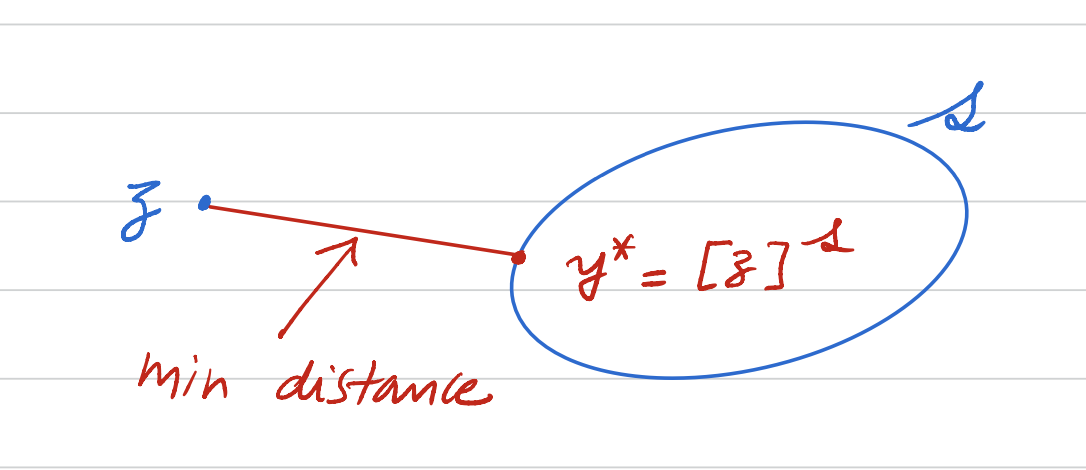
\includegraphics[scale=0.5]{projection1.png}
    \caption{Projection onto Closed Convex Set}
    \label{}
\end{figure}\end{center}
\textbf{Note:} $[z]^\&$ exists and is unique in convex $\&$, however, when $\&$ is not convex, $[z]^\&$ may not be unique.
\begin{center}\begin{figure}[htbp]
    \centering
    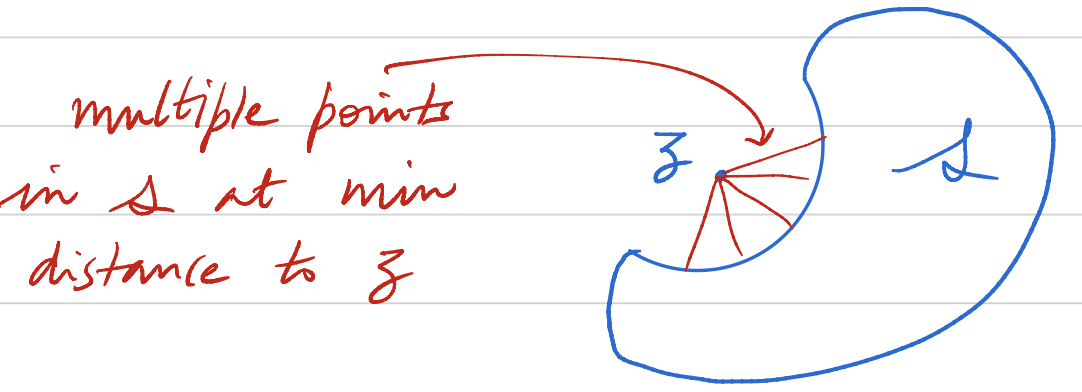
\includegraphics[scale=0.5]{projection2.png}
    \caption{Projection onto Closed non-Convex Set}
    \label{}
\end{figure}\end{center}

\subsection{\underline{Unique} projection $[z]^\&$ on \underline{closed convex} subset of $\mathbb{R}^n$}
\begin{proposition}
    [Existence and Uniqueness of Projection]
    Let $\&$ be a \underline{closed convex} subset of $\mathbb{R}^n$. Then, for every $z\in \mathbb{R}^n$, there exists a unique $[z]^\&$.
\end{proposition}
\begin{proof}
Nee to show that $\min_{y\in \&}\|z-y\|^2$ exists and is unique.

Let $x$ be some element of $\&$. Then
\begin{equation}
    \begin{aligned}
        &\text{minimizing $\|z-y\|^2$ over all $y\in\&$}\\
        \equiv&\text{minimizing $\|z-y\|^2$ over the set $A=\{y\in\&:\|z-y\|^2\}$}
    \end{aligned}
    \nonumber
\end{equation}
$g(y)=\|z-y\|^2$ is strictly convex on set $\&$ $\Rightarrow$ $A$ is a convex set and $g$ is convex on $A$.

Also $g$ is continuous $\Rightarrow	A$ is closed.

Finally, $y\in A \Rightarrow \|y\|^2=\|y-z+z\|^2\leq \|y-z\|^2+\|z\|^2\leq \|z-x\|^2+\|z\|^2 \Rightarrow A$ is bounded.

Thus, $g(y)=\|z-y\|^2$ is strictly convex over set $A$, which is compact.

Therefore, $\min_{y\in\&}\|\&-y\|^2=\min_{y\in A}\|\&-y\|^2$ exists (Weierstrass’ Theorem) and is unique (strict convexity).
\end{proof}

\subsection{Obtuse Angle Criterion: $[z]^\&$ is projection $\Leftrightarrow$ $(z-[z]^\&)^T(y-[z]^\&)\leq 0, \forall y\in\&$}

When solving the closest point problem for a vector space $S=\{\vec{y}:A \vec{y}=\vec{0}\}$ or affine subspace $S=\{\vec{y}:A \vec{y}=\vec{b}\}$, we use \textbf{perpendicularity condition} (orthogonality condition) -i.e., that $\vec{x}^*\cdot \vec{y}=0,\forall \vec{y}\in S$

A weaker form of that condition is the obtuse angle criterion, \textbf{which holds for any convex set}:
\begin{theorem}[Obtuse angle criterion]
    Let $C$ be a convex set and let $\vec{y}$ be a point outside $C$. $\vec{x}^*$ is the closest point in $C$ to $\vec{y}$ \underline{if and only if} $$(\vec{y}-\vec{x}^*)\cdot (\vec{x}-\vec{x}^*)\leq 0,\quad \forall \vec{x}\in C$$
\end{theorem}
\begin{center}\begin{figure}[htbp]
    \centering
    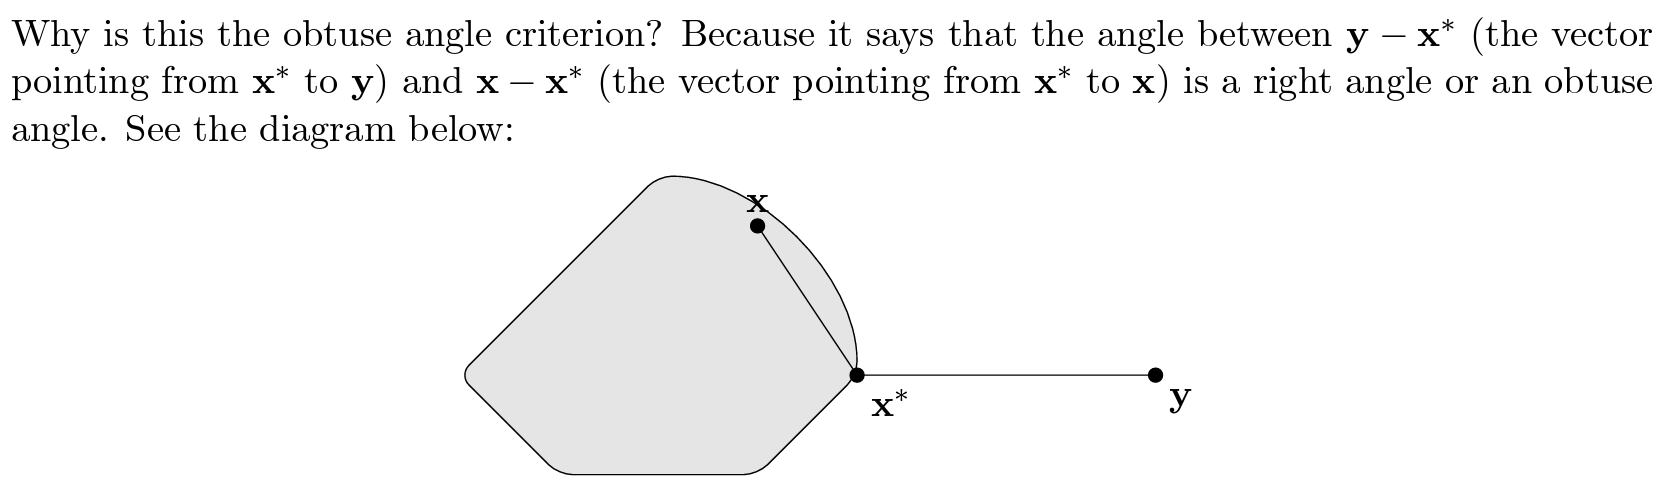
\includegraphics[scale=0.25]{obtuse.png}
    \caption{Obtuse angle criterion}
    \label{}
\end{figure}\end{center}
\textbf{In Projection Form}
\begin{proposition}
    [Necessary and Sufficient Condition for Projection]
    Let $\&$ be a \underline{closed conex} subset of $\mathbb{R}^n$. Then,
    \begin{equation}
        \begin{aligned}
            [z]^\&=y^*
            &\Leftrightarrow (y^*-z)^T(y-y^*)\geq 0,\quad \forall y\in\&.\\
            &\Leftrightarrow (z-y^*)^T(y-y^*)\leq 0,\quad \forall y\in\&.
        \end{aligned}
        \nonumber
    \end{equation}
\end{proposition}
\begin{proof}
    $[z]^\& = \argmin_{y\in\&}g(y)$, with $g(y)=\|z-y\|^2$ (which is strictly convex), $\nabla g(y)=2(y-z)$.

    By the optimality conditions,
    \begin{equation}
        \begin{aligned}
            &y^*\text{ is the unique minimizer of $g(y)$ over $\&$}\\
            \Leftrightarrow	& \nabla g(y^*)^T(y-y^*)\geq 0\quad \forall y\in\&\\
            \Leftrightarrow & (y^*-z)^T(y-y^*)\geq 0,\quad \forall y\in\&.\\
            \Leftrightarrow &(z-y^*)^T(y-y^*)\leq 0,\quad \forall y\in\&.
        \end{aligned}
        \nonumber
    \end{equation}
\end{proof}
\begin{center}\begin{figure}[htbp]
    \centering
    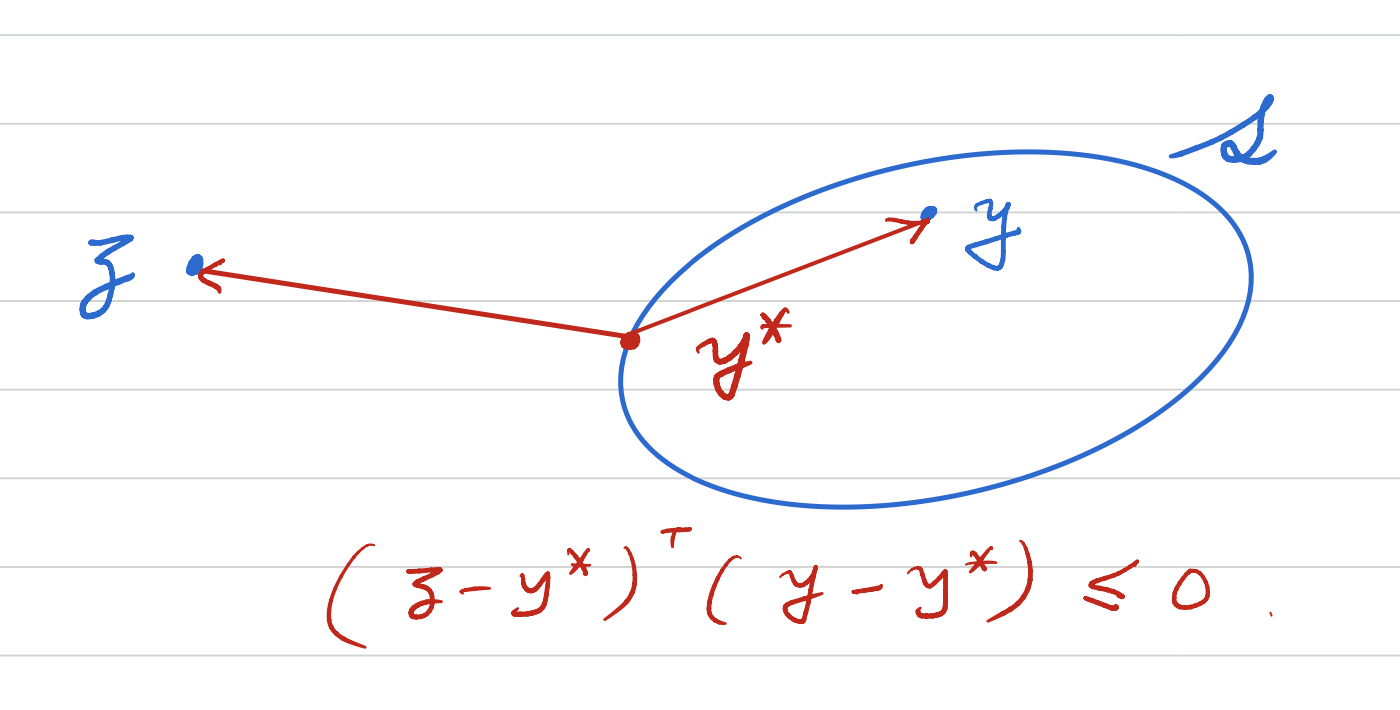
\includegraphics[scale=0.3]{projection3.png}
    \caption{Necessary and Sufficient Condition for Projection}
    \label{}
\end{figure}\end{center}

\subsubsection{Special Case (Linear subspace): Orthogonality Principle $(z-[z]^\&)^Tx= 0,\forall x\in\&$}
Suppose $\&$ is a linear subspace of $\mathbb{R}^n$, any linear combination of points in $\&$ is also in $\&$. Note that $\&$ is \underline{closed and convex}.

Then, for $z\in \mathbb{R}^n$, $[z]^\&=y^*$ satisfies:
\begin{equation}
    \begin{aligned}
        (z-y^*)^T(y-y^*)\leq 0,\quad \forall y\in\&.
    \end{aligned}
    \nonumber
\end{equation}
According to the property of subsapce, we can infer that
\begin{equation}
    \begin{aligned}
        (z-y^*)^Tx\leq 0,\quad \forall x\in\&.
    \end{aligned}
    \nonumber
\end{equation}
$-x$ also in $\&$, $-x\in\& \Rightarrow$
\begin{equation}
    \begin{aligned}
        (z-y^*)^Tx\geq 0,\quad \forall x\in\&.
    \end{aligned}
    \nonumber
\end{equation}
Then we can infer that
\begin{equation}
    \begin{aligned}
        (z-y^*)^Tx= 0,\quad \forall x\in\&.
    \end{aligned}
    \nonumber
\end{equation}
which is called \underline{orthogonality principle}.

\begin{center}\begin{figure}[htbp]
    \centering
    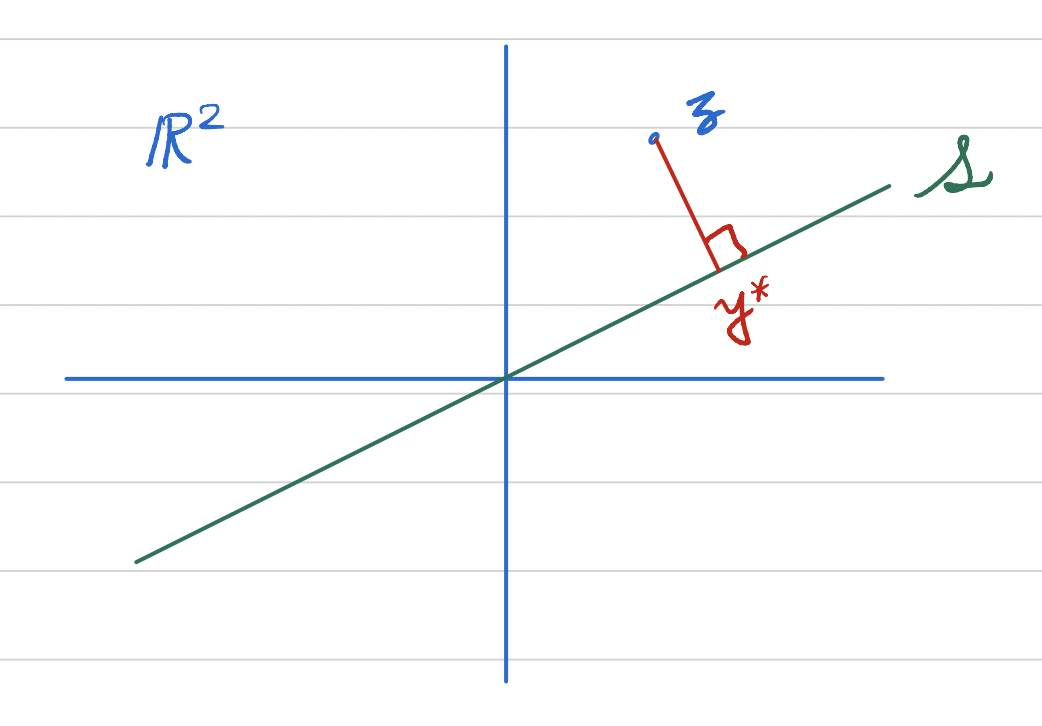
\includegraphics[scale=0.4]{proj1.png}
    \caption{Point from $\mathbb{R}^2$ to $\mathbb{R}$}
    \label{}
\end{figure}\end{center}

\subsection{Prop: Projection is Non-expansive $\|[x]^\&-[z]^\&\|\leq \|x-z\|,\forall x,z\in \mathbb{R}^n$}
\begin{proposition}
    [Projection is non-expansive]
    Let $\&$ be a \underline{closed convex} subset of $\mathbb{R}^n$. Then for $x,z\in \mathbb{R}^n$
    $$\|[x]^\&-[z]^\&\|\leq \|x-z\|\quad \forall x,z\in \mathbb{R}^n$$
\end{proposition}
\begin{proof}
From previous theorem, we know
\begin{equation}
    \begin{aligned}
        (1).\quad ([x]^\&-x)^T(y-[x]^\&)\geq 0,\quad \forall y\in\&.\\
        (2).\quad ([z]^\&-z)^T(y-[z]^\&)\geq 0,\quad \forall y\in\&.\\
    \end{aligned}
    \nonumber
\end{equation}
set $y=[z]^\&$ in (1) and $y=[x]^\&$ in (2), and adding,
\begin{equation}
    \begin{aligned}
        &([z]^\&-[x]^\&)^T([x]^\&-x+z-[z]^\&)\geq 0\\
        \Rightarrow	& ([z]^\&-[x]^\&)^T(z-x)\geq \|[z]^\&-[x]^\&\|^2
    \end{aligned}
    \nonumber
\end{equation}
Applying Cauchy-schwary inequality,
\begin{equation}
    \begin{aligned}
        \|[z]^\&-[x]^\&\|^2&\leq \|[z]^\&-[x]^\&\|\|z-x\|\\
        \|[z]^\&-[x]^\&\|&\leq \|z-x\|
    \end{aligned}
    \nonumber
\end{equation}
\end{proof}

\subsection{The Separation Theorem}
\begin{theorem}[Separation Theorem]
    If $C\subseteq \mathbb{R}^n$ is a closed convex set and $\vec{y}\notin C$, then there is a linear inequality separating $\vec{y}$ from $C$: we can choose $\vec{a}\in \mathbb{R}^n, b\in \mathbb{R}$ such that
    \begin{enumerate}[$\bullet$]
        \item $\vec{a}\cdot \vec{x}\leq b$ for all $\vec{x}\in C$, but
        \item $\vec{a}\cdot \vec{y}> b$
    \end{enumerate}
\end{theorem}
\begin{proof}[Prove by obtuse angle criterion]
    Because $C$ is closed, there is a point $\vec{x}^*\in C$ that is the closest to $\vec{y}$, so
    \begin{equation}
        \begin{aligned}
            (\vec{y}-\vec{x}^*)\cdot (\vec{x}-\vec{x}^*)&\leq 0,\ \forall \vec{x}\in C\\
            (\vec{y}-\vec{x}^*)\cdot \vec{x}&\leq (\vec{y}-\vec{x}^*)\cdot \vec{x}^*
        \end{aligned}
        \nonumber
    \end{equation}
    Let $\vec{a}=\vec{y}-\vec{x}^*$, $b=(\vec{y}-\vec{x}^*)\cdot \vec{x}^*$.
    \begin{equation}
        \begin{aligned}
            \|\vec{y}-\vec{x}\|^2>0 \Rightarrow \vec{a}\cdot\vec{y}>b
        \end{aligned}
        \nonumber
    \end{equation}
\end{proof}
\begin{center}\begin{figure}[htbp]
    \centering
    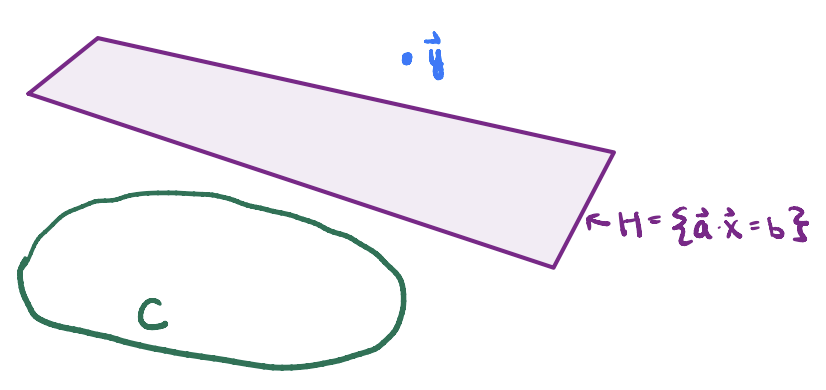
\includegraphics[scale=0.3]{separating.png}
    \caption{separation theorem}
    \label{}
\end{figure}\end{center}

\subsection{Bolzano-Weierstrass theorem}
\subsubsection{Sequence Convergence}
\textbf{\underline{Definition:}} A sequence $\vec{x}_1,\vec{x}_2,\vec{x}_3,...$ of points converges to $\vec{x}^*$ if for any $\varepsilon>0$, there exists some integer $n\in \mathbb{N}$ such that $$\|\vec{x}_m-\vec{x}^*\|<\varepsilon,\ \forall m\geq n$$

\subsubsection{Bolzano-Weierstrass Theorem: Compact set $S$, $\exists$ subsequence converges to $\vec{x}^*\in S$}
\begin{theorem}[Bolzano-Weierstrass]
    Let $S\subseteq \mathbb{R}^n$ be a compact (closed and bounded) set and let $\vec{x}_1,\vec{x}_2,...$ be any sequence of points in $S$.\\
    Then we can choose a subsequence of points that has a limit $\vec{x}^*\in S$. Formally, we can choose indices $i_1<i_2<i_3<\cdots$ such that the sequence $\vec{x}_{i_1},\vec{x}_{i_2},\vec{x}_{i_3},...$ converges to $\vec{x}^*\in S$.
\end{theorem}
\begin{center}
    \fcolorbox{black}{gray!10}{\parbox{.9\linewidth}{\begin{enumerate}[$\bullet$]
        \item "$S$ is bounded" $\Rightarrow$ we can choose a subsequence $\vec{x}_{i_1},\vec{x}_{i_2},\vec{x}_{i_3},...$ converges to $\vec{x}^*\in S$.
        \item "$S$ is closed" $\Rightarrow$ the limit of this subsequence is \underline{in} $S$.
    \end{enumerate}}}
\end{center}

\subsubsection{Extreme Value Theorem: continuous $f$ compact set $\rightarrow \mathbb{R}$ has global-min}
\begin{corollary}[Extreme value theorem]
    If $S\subseteq \mathbb{R}^n$ is a compact (closed and bounded) set and $f: S \rightarrow \mathbb{R}$ is a continuous function, then $f$ has a global maximizer on $S$.
\end{corollary}

\subsubsection{Support Theorem: $z\in bd(C)$, $\exists \vec{u}$ s.t. $\vec{u}\cdot \vec{x}\leq \vec{u}\cdot \vec{z}, \forall \vec{x}\in C$}
\begin{corollary}[Support Theorem]
    Let $C\subseteq \mathbb{R}^n$ be a convex set and $\vec{z}$ be a point in $bd(C)$. Then there is an inequality supporting $C$ at $\vec{z}$ - i.e., we can choose some unit vector $\vec{u}\in \mathbb{R}^n$ such that $$\vec{u}\cdot \vec{x}\leq \vec{u}\cdot \vec{z},\ \forall \vec{x}\in C$$
\end{corollary}
\begin{proof}
    Since $\vec{z}\in bd(C)$, we can find a sequence $\vec{y}^{(1)},\vec{y}^{(2)},...\notin C$ converging to $\vec{z}$. (e.g. let $y^{(k)}$ be one such point: it will satisfy $\|\vec{y}^{(k)}-\vec{z}\|\leq \frac{1}{k}$)\\
    For each $\vec{y}^{(k)}$, there is an inequality separating it from $cl(C)$: some $\vec{a}^{(k)}$ such that $$\vec{a}^{(k)}\cdot \vec{x}< \vec{a}^{(k)}\cdot \vec{y}^{(k)},\ \forall \vec{x}\in C$$
    Dividing by $\|\vec{a}^{(k)}\|$, we get
    \begin{equation}
        \begin{aligned}
            \frac{\vec{a}^{(k)}}{\|\vec{a}^{(k)}\|}\cdot \vec{x}<\frac{\vec{a}^{(k)}}{\|\vec{a}^{(k)}\|}\cdot \vec{y}^{(k)},\ \forall \vec{x}\in C
        \end{aligned}
        \nonumber
    \end{equation}
    so $\vec{u}^{(k)}=\frac{\vec{a}^{(k)}}{\|\vec{a}^{(k)}\|}$ is a vector with $\|\vec{u}\|=1$ that satisfies $$\vec{u}^{(k)}\cdot \vec{x}<\vec{u}^{(k)}\cdot \vec{y}^{(k)},\ \forall \vec{x}\in C$$
    The points $\vec{u}^{(1)},\vec{u}^{(2)},...$ are a sequence of points in the closed and bounded set $\{x \in \mathbb{R}^n : \|x\|= 1\}$. This means we can pick out a subsequence of them converging to some $u\in \mathbb{R}^n$ with $\|u\|= 1$.\\
    Taking the limit of the inequality $\vec{u}^{(k)}\cdot \vec{x}<\vec{u}^{(k)}\cdot \vec{y}^{(k)}$ for this subsequence, we get $$\vec{u}\cdot \vec{x}\leq \vec{u}\cdot \vec{z},\ \forall \vec{x}\in C$$
\end{proof}


\section{Constrained Optimization}
\underline{General Form of Constrained Optimization:} A nonlinear program $P$
\begin{equation}
    \begin{aligned}
        \min_{\vec{x}\in S}&\quad &f(\vec{x})\\
        s.t.& &\vec{g}(\vec{x})\leq \vec{0}
    \end{aligned}
    \nonumber
\end{equation}
where we think of $\vec{g}(\vec{x}): S \rightarrow \mathbb{R}^m$ as a vector-valued function $\vec{g}(\vec{x})=\left(g_1(\vec{x}),...,g_m(\vec{x})\right)$.
\begin{enumerate}
    \item \textbf{Feasible region:} $F=\{\vec{x}\in S: \vec{g}(\vec{x})\leq \vec{0}\}$. A point $\vec{x}\in F$ is called a \textbf{feasible solution} of $P$
    \item The \textbf{value} of $P$ is $MP=\inf\{f(\vec{x}): \vec{x}\in F\}$
\end{enumerate}
Note:
\begin{enumerate}[$\bullet$]
    \item If $P$ is unbounded, and $f(\vec{x})$ can be made arbitrarily negative, then $MP = -\infty$. If $P$ is inconsistent, and $F$ is empty, then $MP = +\infty$.
    \item If $P$ has solutions getting arbitrarily close to a value $z$, but are always bigger than $z$, then $MP =z$ as well.
\end{enumerate}

\begin{definition}
    A nonlinear program $P$ is a \textbf{convex program} if: 1. The set $S$ is convex; 2. All the function $f,g_1,...,g_m$ are convex functions.
\end{definition}

\subsection{Perturbation of Constraints}
\textbf{Sensitivity Analysis:} we want to understand how sensitive MP is to slight changes in the constraints - this tells us which constraints "matter".

Generalize $P$ to the \textbf{perturbation} $P(\vec{z})$:
\begin{equation}
    \begin{aligned}
        \min_{\vec{x}\in S}&\quad &f(\vec{x})\\
        s.t.& &\vec{g}(\vec{x})\leq \vec{z}
    \end{aligned}
    \nonumber
\end{equation}
where $\vec{z}=(z_1,...,z_m)$

\begin{definition}
    For $P(\vec{z})$, we define $F(\vec{z}):=\{\vec{x}: \vec{x}\in S \text{ and }\vec{g}(\vec{x})\leq \vec{z}\}$ (feasible region); $MP(\vec{z}):=\inf\{f(\vec{x}):\vec{x}\in F(\vec{z})\}$ (value function)
\end{definition}

\subsubsection{Theorem: convex program $\Rightarrow$ $MP(\vec{z})$ is a convex function on convex domain}
\begin{center}
    \fcolorbox{black}{blue!10}{\parbox{.9\linewidth}{\begin{theorem}
        Let $P$ be a convex program. Then the domain of $MP(\vec{z})$ (the set of $\vec{z}$ for which $MP(\vec{z})$ is feasible) is a convex set, and $MP(\vec{z})$ is a convex function on that domain.
    \end{theorem}}}
\end{center}
\begin{example}
    Consider the convex program
    \begin{equation}
        \begin{aligned}
            \min_{(x,y)\in \mathbb{R}^2}&\quad &|x-1|\\
            s.t.& &\sqrt{x^2+y^2}\leq 0
        \end{aligned}
        \nonumber
    \end{equation}
    Here $P(\vec{z})$ is the program:
    \begin{equation}
        \begin{aligned}
            \min_{(x,y)\in \mathbb{R}^2}&\quad &|x-1|\\
            s.t.& &\sqrt{x^2+y^2}\leq z
        \end{aligned}
        \nonumber
    \end{equation}
\end{example}
\begin{enumerate}
    \item For $z<0$, there are \underline{no} feasible points, so $MP(z)=+\infty$ and were outside the domain of MP.
    \item For $0\leq z<1$, the best we can do is the point $(x,y)=(z,0)$, then $MP(z)=|z-1|=1-z$.
    \item For $z\geq 1$, the point $(1,0)$ is feasible for $P(z)$, we can make $MP(z)=0$.
\end{enumerate}

\subsection{Karush-Kuhn-Tucker theorem}
Intuitively, knowing that $MP(\vec{z})$ is a convex function tells us that it cannot decrease too quickly. So if we make $P$ an unconstrained program, allowing $\vec{x}$ to violate the constraint $g(\vec{x}) \leq \vec{0}$, then a small violation in the constraint can only yield a small improvement. If we modify the objective function $f(\vec{x})$ to take that into account the small change, we can forget about the constraints at all.

\subsubsection{Def: $P$ is super-consistent (Slater's condition): $\exists \vec{x}^*\in S$ s.t. $\vec{g}(\vec{x}^*)<\vec{0}$}
\begin{definition}
    If there exists some $\vec{x}^*\in S$ such that $\vec{g}(\vec{x}^*)<\vec{0}$, we say $P$ is \textbf{super-consistent}. This condition is also known as \textbf{Slater's condition}.
\end{definition}

\subsubsection{Lemma: Convex $P$ is super-consistent $\Rightarrow$ $\exists$ sensitivity vector $\vec{\lambda}\geq 0$ s.t. $MP(\vec{z})\geq MP(\vec{0})-\vec{\lambda}\cdot \vec{z},\forall \vec{z}$}
\begin{center}
    \fcolorbox{black}{blue!5}{\parbox{.9\linewidth}{\begin{lemma}[Sensitivity vector lemma]
        Let $P$ be a convex program with a point $\vec{x}^*\in S$ such that $\vec{g}(\vec{x}^*)< \vec{0}$ (Slater's condition, which makes sure $\vec{0}$ is an interior point of $MP$'s domain).\\
        Then there exists some $\vec{\lambda}\in \mathbb{R}^m$ with $\vec{\lambda}\geq \vec{0}$ such that $$MP(\vec{z})\geq MP(\vec{0})-\vec{\lambda}\cdot \vec{z},\quad \forall \vec{z}$$
        A vector $\vec{\lambda}\in \mathbb{R}^m$ with $\vec{\lambda}\geq \vec{0}$ satisfying this inequality is called a \textbf{sensitivity vector}: it measures the sensitivity of $P$ to changes in the constraints.
    \end{lemma}}}
\end{center}
\begin{proof}
    If $\vec{0}$ is an interior point of the domain of MP, then MP has a sub-gradient at $\vec{0}$. So, $\exists \vec{d}$
    \begin{equation}
        \begin{aligned}
            MP(\vec{z})\geq MP(\vec{0})+\vec{d}\cdot(\vec{z}-\vec{0})=MP(\vec{0})+\vec{d}\cdot\vec{z}
        \end{aligned}
        \nonumber
    \end{equation}
    Take $\vec{z}=\vec{e}^{(i)}$, we have $$MP(\vec{e}^{(i)})\geq MP(\vec{0})+\vec{d}\cdot \vec{e}^{(i)}=MP(\vec{0})+d_i$$
    On the other hand, $MP(\vec{0})\geq MP(\vec{e}^{(i)})$, so $$MP(\vec{0})\geq MP(\vec{e}^{(i)})\geq MP(\vec{0})+d_i \Rightarrow d_i\leq 0$$
    Hence, there exists $\lambda=-\vec{d}\geq \vec{0}$
\end{proof}


\subsubsection{Goalposts Lemma: $\vec{x}^{(0)}$ is feasible for $P(\vec{g}(\vec{x}^{(0)}))$ and $MP(\vec{g}(\vec{x}^{(0)}))\leq f(\vec{x}^{(0)})$}
\begin{center}
    \fcolorbox{black}{blue!5}{\parbox{.9\linewidth}{\begin{lemma}[“Moving the goalposts” lemma]
        Let $P$ be any nonlinear program. For any $\vec{x}^{(0)}\in S$,
        \begin{enumerate}[(a)]
            \item $\vec{x}^{(0)}$ is feasible for $P(\vec{g}(\vec{x}^{(0)}))$ and
            \item $MP(\vec{g}(\vec{x}^{(0)}))\leq f(\vec{x}^{(0)})$
        \end{enumerate}
    \end{lemma}}}
\end{center}
The second lemma says that any element of $S$, even if it's not feasible for $P$, still gives a bound on $MP(\vec{z})$ for some $\vec{z}$, and therefore (by the first lemma) it still gives a bound on $MP(0)$, the minimum value of $P$.
\begin{proof}
    $P(g(\vec{x}^{(0)}))$ is
    \begin{equation}
        \begin{aligned}
            \min_{\vec{x}\in S}&\quad &f(\vec{x})\\
            s.t.& &\vec{g}(\vec{x})\leq g(\vec{x}^{(0)})
        \end{aligned}
        \nonumber
    \end{equation}
    (a), (b) are obvious.
\end{proof}

\subsubsection{KKT Theorem: Saddle Point Form}
\begin{definition}
    Given $\vec{x}\in S$ and $\vec{\lambda}\in \mathbb{R}^m$, the \textbf{Lagrangian} is
    \begin{equation}
        \begin{aligned}
            L(\vec{x},\vec{\lambda})=f(\vec{x})+\vec{\lambda}\cdot \vec{g}(\vec{x})=f(\vec{x})+\sum_{i=1}^m\lambda_i g_i (\vec{x})
        \end{aligned}
        \nonumber
    \end{equation}
\end{definition}
The textbook states it for all convex programs satisfying the Slater condition: convex programs with a point satisfying all constraints strictly (with a $<$ in place of a $\leq$).
\begin{center}
    \fcolorbox{black}{blue!10}{\parbox{.9\linewidth}{\begin{theorem}[Karush-Kuhn-Tucker theorem, saddle point form]
        Let P be any nonlinear program. Suppose that $\vec{x}^* \in S$ and $\vec{\lambda}^* \geq 0$. Then $\vec{x}^*$ is an optimal solution of $P$ and $\vec{\lambda}^*$ is a sensitivity vector for $P$ if and only if:
        \begin{enumerate}[(1)]
            \item $L(\vec{x}^*,\vec{\lambda}^*)\leq L(\vec{x},\vec{\lambda}^*)$ for all $\vec{x}\in S$. (minimality of $\vec{x}^*$)
            \item $L(\vec{x}^*,\vec{\lambda}^*)\geq L(\vec{x}^*,\vec{\lambda})$ for all $\vec{\lambda}\geq \vec{0}$. (maximality of $\vec{\lambda}^*$)
            \item $\lambda_i^* g_i(\vec{x}^*)=0$ for $i=1,...,m$. (complementary slackness)
        \end{enumerate}
    \end{theorem}}}
\end{center}

\begin{proof}\quad
    \begin{enumerate}[$\bullet$]
        \item $(\Rightarrow):$ Assume $\vec{x}^*$ is an optimal solution of $P$ and $\vec{\lambda}^*\geq 0$ is a sensitivity vector. Take $\vec{x}\in S$, then
        \begin{equation}
            \begin{aligned}
                f(\vec{x})&\geq MP(\vec{g}(\vec{x}))\quad \text{(goalpost lemma)}\\
                &\geq MP(\vec{0})-\vec{\lambda}^*\cdot \vec{g}(\vec{x})\quad \text{(sensitivity vector lemma)}\\
                &=f(\vec{x}^*)-\vec{\lambda}^*\cdot \vec{g}(\vec{x})\quad \text{(by definition of $\vec{x}^*$ and $MP(\vec{0})$)}
            \end{aligned}
            \nonumber
        \end{equation}
        Rearranging,
        \begin{equation}
            \begin{aligned}
                f(\vec{x}^*)\leq f(\vec{x})+\vec{\lambda}^*\cdot \vec{g}(\vec{x})=L(\vec{x},\vec{\lambda}^*)\quad \text{(definition of Lagrangian)}
            \end{aligned}
            \nonumber
        \end{equation}
        If we set $\vec{x}=\vec{x}^*$, $$\vec{\lambda}^*\cdot \vec{g}(\vec{x}^*)\geq 0$$
        Since $\vec{\lambda}^*\geq 0, \vec{g}(\vec{x}^*)\leq 0$ (feasible point),
        \begin{equation}
            \begin{aligned}
                &&\vec{\lambda}^*\cdot \vec{g}(\vec{x}^*)&\leq 0&\\
               &\Rightarrow& \vec{\lambda}^*\cdot \vec{g}(\vec{x}^*)&= 0&\\
               &\Rightarrow& L(\vec{x}^*,\vec{\lambda}^*)&=f(\vec{x}^*)\leq L(\vec{x},\vec{\lambda}^*)&\\
            \end{aligned}
            \nonumber
        \end{equation}
        Similarly, $\forall \vec{\lambda}\geq 0$,
        \begin{equation}
            \begin{aligned}
                &&\vec{\lambda}\cdot \vec{g}(\vec{x}^*)&\leq 0=\vec{\lambda}^*\cdot \vec{g}(\vec{x}^*)&\\
               &\Rightarrow& L(\vec{x}^*,\vec{\lambda})&\leq L(\vec{x}^*,\vec{\lambda}^*)&\\
            \end{aligned}
            \nonumber
        \end{equation}
        \item ($\Leftarrow$): For $1\leq i\leq m$, take $\vec{\lambda}=\vec{\lambda}^*+\vec{e}^{(i)}$. Then,
        \begin{equation}
            \begin{aligned}
                L(\vec{x}^*,\vec{\lambda})&=f(\vec{x}^*)+\left(\vec{\lambda}^*+\vec{e}^{(i)}\right)\cdot \vec{g}(\vec{x}^*)\\
                &=f(\vec{x}^*)+\vec{\lambda}^*\cdot \vec{g}(\vec{x}^*)+ g_i(\vec{x}^*)\\
                &=L(\vec{x}^*,\vec{\lambda}^*)+g_i(\vec{x}^*)\\
                \text{by (2) }\Rightarrow\ &g_i(\vec{x}^*)\leq 0,\quad \forall 1\leq i\leq m
            \end{aligned}
            \nonumber
        \end{equation}
        Hence, $\vec{x}^*$ is feasible in $P$.

        For any $\vec{x}\in S$,
        \begin{equation}
            \begin{aligned}
                f(\vec{x})&\geq f(\vec{x})+\sum_{i=1}^m\lambda_i^* g_i(\vec{x})\\
                &=L(\vec{x},\vec{\lambda}^*)\\
                &\geq L(\vec{x}^*,\vec{\lambda}^*)\\
                &=f(\vec{x}^*)+\sum_{i=1}^m\lambda_i^* g_i(\vec{x}^*)\\
                &=f(\vec{x}^*)
            \end{aligned}
            \nonumber
        \end{equation}
        Hence, $\vec{x}^*$ is optimal.

        Let $\vec{x}'$ be the optimal point of $P(\vec{z})$, so $\vec{x}'\in S$ and $\vec{g}(\vec{x}')\leq \vec{z}$. Then,
        \begin{equation}
            \begin{aligned}
                MP(\vec{0})=f(\vec{x}^*)&=L(\vec{x}^*,\vec{\lambda}^*)\\
                &\leq L(\vec{x}',\vec{\lambda}^*)\\
                &= f(\vec{x}')+\vec{\lambda}^*\cdot \vec{g}(\vec{x}')\\
                &\leq f(\vec{x}')+\vec{\lambda}^*\cdot \vec{z}\\
                &=MP(\vec{z})+\vec{\lambda}^*\cdot \vec{z}
            \end{aligned}
            \nonumber
        \end{equation}
        Hence, $MP(\vec{z})\geq MP(\vec{0})-\vec{\lambda}^*\cdot \vec{z}$ which denotes $\vec{\lambda}^*$ is a sensitivity vector.
    \end{enumerate}
\end{proof}

\subsubsection{KKT Theorem: Gradient Form}
\begin{center}
    \fcolorbox{black}{blue!10}{\parbox{.9\linewidth}{\begin{theorem}[Karush-Kuhn-Tucker theorem, gradient form]
        Let P be any nonlinear program where $f$ and $g_1,...,g_m$ have continuous first partial derivatives. Suppose that $\vec{x}^* \in int (S)$ is an optimal solution of $P$, and $\vec{\lambda}^* \geq 0$ is a sensitivity vector. Then:
        \begin{enumerate}[(1)]
            \item $\nabla_{\vec{x}} L(\vec{x}^*,\vec{\lambda}^*)=\vec{0}$. That is, $\nabla f(\vec{x}^*)+\sum_{i=1}^m\lambda_i^* \nabla g_i(\vec{x}^*)=\vec{0}$
            \item For each $1\leq i\leq m$, $g_i(\vec{x}^*)\leq 0$.
            \item For each $1\leq i\leq m$, either $\lambda_i^*=0$ or $g_i(\vec{x}^*)=0$.
        \end{enumerate}
        \textbf{Furthermore,} if $P$ is a convex program then the converse holds: If $(\vec{x}^*,\vec{\lambda}^*)$ satisfy these conditions $\Rightarrow$ $\vec{x}^*$ is an optimal solution and $\vec{\lambda}^*$ is a sensitivity vector.
    \end{theorem}}}
\end{center}
Using KKT gradient form to solve program:
\begin{enumerate}[$\bullet$]
    \item We need $P$ be convex and super-consistent $\Rightarrow$ $\exists$ sensitivity vector.\\
    We need $P$ have optimal solution.
    \item Then, we can use the three conditions to find the optimal $\vec{x}^*$ and sensitivity $\vec{\lambda}^*$.
\end{enumerate}

\textbf{Example:} Consider the $(P)$
\begin{equation}
    \begin{aligned}
        \min_{\vec{x}\in S}\quad &\frac{1}{x+y}\\
        s.t.\quad & 2x+y^2-6\leq 0\\
        & 1-x\leq 0\\
        & 1-y\leq 0
    \end{aligned}
    \nonumber
\end{equation}
where $S=\{(x,y):x,y>0\}$.

$\nabla f(x,y)=\begin{bmatrix}
    -\frac{1}{(x+y)^2}\\-\frac{1}{(x+y)^2}
\end{bmatrix}$, $\nabla^2 f(x,y)=\begin{bmatrix}
    \frac{2}{(x+y)^3}&\frac{2}{(x+y)^3}\\
    \frac{2}{(x+y)^3}&\frac{2}{(x+y)^3}
\end{bmatrix}\succeq 0$.

$\nabla g_1(x,y)=\begin{bmatrix}
    2\\2y
\end{bmatrix}$, $\nabla g_2(x,y)=\begin{bmatrix}
    -1\\0
\end{bmatrix}$, $\nabla g_3(x,y)=\begin{bmatrix}
    0\\-1
\end{bmatrix}$.

We can know $(P)$ is a convex program; If $\vec{x}=(1.5,1.5)$, $\vec{g}(\vec{x})\leq\vec{0}$ $\Rightarrow$ $(P)$ is super-consistent: we can use KKT theorem to solve the problem.
\begin{enumerate}[$\bullet$]
    \item $\nabla_{\vec{x}} L(\vec{x},\vec{\lambda})=\vec{0}$
    \begin{equation}
        \begin{aligned}
            \begin{bmatrix}
                -\frac{1}{(x+y)^2}\\-\frac{1}{(x+y)^2}
            \end{bmatrix}+\lambda_1 \begin{bmatrix}
                2\\2y
            \end{bmatrix}+ \lambda_2 \begin{bmatrix}
                -1\\0
            \end{bmatrix}+ \lambda_3 \begin{bmatrix}
                0\\-1
            \end{bmatrix}=\vec{0}
        \end{aligned}
        \nonumber
    \end{equation}
    \item If $\lambda_1=0$, $\lambda_2=\lambda_3=-\frac{1}{(x+y)^2}<0$ must be satisfied, which contradicts to condition $\vec{\lambda}\geq 0$.
    \item Since $\lambda_1\neq 0$, $2x+y^2-6=0$ must hold.
    \item If $x=1$ holds, $y=2$ (which also implies $\lambda_3=0$). Then
    \begin{equation}
        \begin{aligned}
            \begin{bmatrix}
                -\frac{1}{9}\\-\frac{1}{9}
            \end{bmatrix}+\lambda_1 \begin{bmatrix}
                2\\4
            \end{bmatrix}+ \lambda_2 \begin{bmatrix}
                -1\\0
            \end{bmatrix}=\vec{0}
        \end{aligned}
        \nonumber
    \end{equation}
    This gives us $\lambda_1=\frac{1}{36}$ and $\lambda_2=-\frac{1}{18}$, which contradicts to $\vec{\lambda}\geq 0$. Since $x\neq 1$, $\lambda_2=0$.
    \item If $y=1$ holds, $x=\frac{5}{2}$ (which also implies $\lambda_2=0$)
    \begin{equation}
        \begin{aligned}
            \begin{bmatrix}
                -\frac{1}{{3.5}^2}\\-\frac{1}{{3.5}^2}
            \end{bmatrix}+\lambda_1 \begin{bmatrix}
                2\\2
            \end{bmatrix}+ \lambda_3 \begin{bmatrix}
                0\\-1
            \end{bmatrix}=\vec{0}
        \end{aligned}
        \nonumber
    \end{equation}
    This gives us $\lambda_1=\frac{2}{49}$ and $\lambda_3=0$, satisfying all the conditions.
\end{enumerate}
According to KKT theorem, $\vec{x}=(\frac{5}{2},1)$ and $\vec{\lambda}=(\frac{2}{49},0,0)$ is the optimal solution.

\subsubsection{Relationship between KKT and Optimal Solution}
\begin{center}\begin{figure}[htbp]
    \centering
    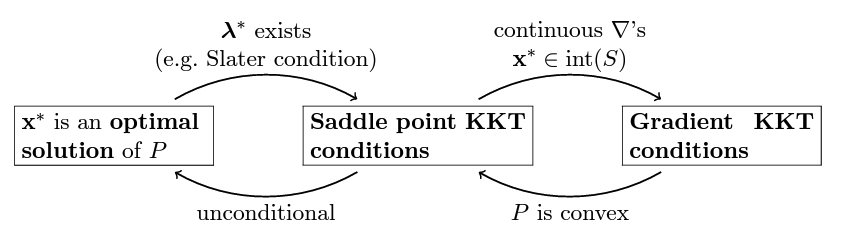
\includegraphics[scale=0.4]{KKT_opt.png}
    \caption{Relationship between KKT and Optimal Solution}
    \label{}
\end{figure}\end{center}

\subsection{KKT Duality}

\subsubsection{Thm: If $P$ has optimal solution $\vec{x}^*$ and sensitivity vector $\vec{\lambda}^*$, $h(\vec{\lambda})=\inf_{\vec{x}\in S}\{L(\vec{x},\vec{\lambda})\}\leq h(\vec{\lambda^*})=f(\vec{x}^*), \forall \vec{\lambda}$}
Define $h(\vec{\lambda})=\inf_{\vec{x}\in S}\{L(\vec{x},\vec{\lambda})\}$

Note that:\begin{enumerate}[$\bullet$]
    \item If $L(\vec{x},\vec{\lambda})$ is not bounded below on $S$, we set $h(\vec{\lambda})=-\infty$.
    \item If $S$ is an empty set, we set $h(\vec{\lambda})=+\infty$.
    \item If $L(\vec{x},\vec{\lambda})$ has solutions getting arbitrarily close to a value $z$, but are always bigger than $z$, then $h(\vec{\lambda})=z$ as well.
\end{enumerate}

\begin{center}
    \fcolorbox{black}{blue!10}{\parbox{.9\linewidth}{\begin{theorem}[KKT Duality]
        Suppose that $P$ has an optimal solution $\vec{x}^*\in S$ and a sensitivity vector $\vec{\lambda}^*\geq \vec{0}$. Then for all $\vec{\lambda}\geq \vec{0}$, $$h(\vec{\lambda})\leq h(\vec{\lambda}^*)=f(\vec{x}^*)$$
        \end{theorem}
        This theorem shows that $h(\vec{\lambda})$ provides a lower bound for the value of the objective function.}}
\end{center}
\textbf{Note:} $h(\vec{\lambda}^*)=f(\vec{x}^*)$ need the (1)\underline{existence of optimal solution} and sensitivity vector. To guarantee the existence of sensitivity vector, we need to show (2)\underline{$P$ is convex} and (3)\underline{super-consistent}.
\begin{proof}
    According to KKT's (1), $L(\vec{x}^*,\vec{\lambda}^*)\leq L(\vec{x},\vec{\lambda}^*)$, we have $$h(\vec{\lambda}^*)=L(\vec{x}^*,\vec{\lambda}^*)$$
    According to KKT's (3), $\lambda_i^* g_i(\vec{\lambda}^*)=0,\forall i$, $$h(\vec{\lambda}^*)=L(\vec{x}^*,\vec{\lambda}^*)=f(\vec{x}^*)+\sum_{i=1}^m\lambda_i^* g_i(\vec{\lambda}^*)=f(\vec{x}^*)$$
    According to KKT's (3), $L(\vec{x}^*,\vec{\lambda})\leq L(\vec{x}^*,\vec{\lambda}^*)$, $$h(\vec{\lambda})=\inf_{\vec{x}\in S}\{L(\vec{x},\vec{\lambda})\}\leq L(\vec{x}^*,\vec{\lambda})\leq L(\vec{x}^*,\vec{\lambda}^*)=h(\vec{\lambda}^*)$$
\end{proof}

\subsubsection{KKT Duality}
\begin{center}
    \fcolorbox{black}{blue!5}{\parbox{.9\linewidth}{This motivates us to define the dual program $D$ as:
    \begin{equation}
        \begin{aligned}
            (D)\quad \left\{\begin{matrix}
                \max_{\vec{\lambda}\in \mathbb{R}^m}&h(\vec{\lambda})=\inf_{\vec{x}\in S} L(\vec{x},\vec{\lambda})\\
                s.t.&\vec{\lambda}\geq \vec{0}
            \end{matrix}\right.
        \end{aligned}
        \nonumber
    \end{equation}}}
\end{center}
\textbf{Example:}
\begin{equation}
    \begin{aligned}
        (P)\quad \left\{\begin{matrix}
            \min_{(x,y)\in \mathbb{R}^2}&x^2+y^2\\
            s.t.&x+2y\geq 4
        \end{matrix}\right.
    \end{aligned}
    \nonumber
\end{equation}
$h(\vec{\lambda})=\inf_{(x,y)\in \mathbb{R}^2} x^2+y^2+\lambda (4-x-2y)=4\lambda-\frac{5}{4}\lambda^2$. So the dual problem is
\begin{equation}
    \begin{aligned}
        (D)\quad \left\{\begin{matrix}
            \max_{{\lambda}\in \mathbb{R}}&4\lambda-\frac{5}{4}\lambda^2\\
            s.t.&{\lambda}\geq 0
        \end{matrix}\right.
    \end{aligned}
    \nonumber
\end{equation}
We can solve $\lambda^*=\frac{8}{5}$ and $(x^*,y^*)=\left(\frac{4}{5},\frac{8}{5}\right)$.

\subsubsection{The Duality Gap}
\textbf{Definition:}
\begin{enumerate}
    \item The relationship $h(\vec{\lambda})\leq f(\vec{x})$, when $\vec{x}$ and $\vec{\lambda}$ are feasible for their respective programs, is called \textbf{weak duality}.
    \item We might have $h(\vec{\lambda})< f(\vec{x})$. We refer to such a gap between the largest possible value of $h$ and smallest possible value of $f$ as a \textbf{duality gap}.
\end{enumerate}

When we \underline{do} have a sensitivity vector, then \textbf{strong duality} holds, and we have the equality $f(\vec{x})=h(\vec{\lambda})$ for some primal feasible $\vec{x}$ and dual feasible $\vec{\lambda}$ - such $\vec{x}$ and $\vec{\lambda}$ are optimal.

\begin{definition}
    $MP=\inf\{f(\vec{x}):\vec{x}\in S, \vec{g}(\vec{x})\leq \vec{0}\}$, $MD=\sup\{h(\vec{\lambda}):\vec{\lambda}\geq \vec{0}\}$.
\end{definition}
We have $MP\geq MD$. If $MP\neq MD$, we say there is a duality gap.

\subsection{With Equality Constraints}
Consider
\begin{equation}
    \begin{aligned}(P)\quad
        \left\{\begin{matrix}
        \min_{\vec{x}\in \mathbb{R}^n}& f(\vec{x})\\
        s.t.& \vec{g}(\vec{x})=\vec{0}
        \end{matrix}\right.
    \end{aligned}
    \nonumber
\end{equation}
which equals to
\begin{equation}
    \begin{aligned}(P')\quad
        \left\{\begin{matrix}
        \min_{\vec{x}\in \mathbb{R}^n}& f(\vec{x})\\
        s.t.& \vec{g}(\vec{x})\leq\vec{0}\\
        & -\vec{g}(\vec{x})\leq\vec{0}
        \end{matrix}\right.
    \end{aligned}
    \nonumber
\end{equation}
The Lagrangian of $P'$ is
\begin{equation}
    \begin{aligned}
        L(\vec{x},\lambda_1,\lambda_2)=f(\vec{x})+(\lambda_1-\lambda_2)g(\vec{x})
    \end{aligned}
    \nonumber
\end{equation}
We can define a new variable $\mu=\lambda_1-\lambda_2$ which can be any real number.

\textbf{Dual variables that correspond to equality constraints can be any real number.}

More general we define a non-linear program:
\begin{equation}
    \begin{aligned}(P)\quad
        \left\{\begin{matrix}
        \min_{\vec{x}\in \mathbb{R}^n}& f(\vec{x})\\
        s.t.& g_i(\vec{x})\leq 0,\quad i=1,2,...,m\\
        & h_j(\vec{x})=0,\quad j=1,2,...,l
        \end{matrix}\right.
    \end{aligned}
    \nonumber
\end{equation}
\subsubsection{KKT with equality constraints}
Then the saddle-point version KKT can be written as:
\begin{center}
    \fcolorbox{black}{blue!10}{\parbox{.9\linewidth}{\begin{theorem}[Karush-Kuhn-Tucker theorem, saddle point form]
        Let P be any nonlinear program. Suppose that $\vec{x}^* \in S$ and $\vec{\lambda}^* \geq \mathbb{R}^m$ with $\vec{\lambda}^*\geq \vec{0}$, and $\vec{\mu}^*\in \mathbb{R}^l$. If:
        \begin{enumerate}[(1)]
            \item $L(\vec{x}^*,\vec{\lambda}^*,\vec{\mu}^*)\leq L(\vec{x},\vec{\lambda}^*,\vec{\mu}^*)$ for all $\vec{x}\in S$. (minimality of $\vec{x}^*$)
            \item $L(\vec{x}^*,\vec{\lambda}^*,\vec{\mu}^*)\geq L(\vec{x}^*,\vec{\lambda},\vec{\mu})$ for all $\vec{\lambda}\geq \vec{0}$. (maximality of $(\vec{\lambda}^*,\vec{\mu}^*)$)
            \item $\lambda_i^* g_i(\vec{x}^*)=0$ for $i=1,...,m$. (complementary slackness)
            \item $h_j(\vec{x}^*)=0$ for $j=1,...,l$
        \end{enumerate}
        Then $\vec{x}^*$ is an optimal solution of $P$.
    \end{theorem}}}
\end{center}
The change of gradient form of KKT is similarly updated.

\subsubsection{Equality constraints in the penalty method}
\begin{equation}
    \begin{aligned}(P')\quad
        \left\{\begin{matrix}
        \min_{\vec{x}\in \mathbb{R}^n}& f(\vec{x})\\
        s.t.& h(\vec{x})\leq\vec{0}\\
        & -h(\vec{x})\leq\vec{0}
        \end{matrix}\right.
    \end{aligned}
    \nonumber
\end{equation}
\begin{equation}
    \begin{aligned}
        F_k(\vec{x})&=f(\vec{x})+k\left[((-h)^+(\vec{x}))^2+(h^+(\vec{x}))^2\right]\\
        &=f(\vec{x})+k(h(\vec{x}))^2
    \end{aligned}
    \nonumber
\end{equation}
In general:
\begin{equation}
    \begin{aligned}
        F_k(\vec{x})&=f(\vec{x})+k\left[\sum_{i=1}^m\left(g_i^+(\vec{x})\right)^2+\sum_{j=1}^l(h_j(\vec{x}))^2\right]
    \end{aligned}
    \nonumber
\end{equation}



\subsubsection{More general super-consistent}
\begin{definition}
Suppose $P$ is convex: $S$ is a convex set; the functions $f,g_1,...,g_m$ are all convex; and the functions $h_1,...,h_l$ are all linear (potential with constant terms). Then $P$ is super-consistent if there exists $\vec{x}\in S$ with $g_i(\vec{x})<0$ for all $i=1,...,m$.
\end{definition}
\textbf{Intuitively-} we define convex programs that way because we want both $h_i$ and $-h_i$ to be convex functions $\Rightarrow$ $h_i$ be linear.
\begin{center}
    \fcolorbox{black}{blue!10}{\parbox{.9\linewidth}{\begin{theorem}
        If $P$ is super-consistent and $\vec{x}^*$ is an optimal solution of $P$, then there exists vectors $\vec{\lambda,\vec{\mu}}$ that together with $\vec{x}^*$ satisfy the conditions of the saddle point version of the KKT theorem.
    \end{theorem}}}
\end{center}

\textbf{Essentially-} when we add linear equality constraints, we are optimizing over an affine subspace of $\mathbb{R}^n$ that looks like $\mathbb{R}^k$ for some $k\leq n$. In this subspace, we can apply the usual forms of the KKT theorem and the Slater condition.

\subsubsection{Equality constraints in geometric programming}
\begin{equation}
    \begin{aligned}(GP)\quad
        \left\{\begin{matrix}
        \min_{\vec{t}\in \mathbb{R}^n}& g_0(\vec{t})\\
        s.t.& g_i(\vec{t})\leq 1,\quad i=1,...,m\\
        &\vec{t}\geq 0
        \end{matrix}\right.
    \end{aligned}
    \nonumber
\end{equation}
where $g_0,...,g_m$ are posynomials.

How can we manipulate various types of constants so that they match this standard form?

\begin{center}
    \fcolorbox{black}{gray!10}{\parbox{.9\linewidth}{There is some flexibility here. For any $C>0$, we can deal with the constraint $g(\vec{t}) \leq C$, by rewriting it as $C^{-1} g(\vec{t}) \leq 1$

    But this cannot be done with a negative $C$, because the coefficients in a posynomial cannot be positive. Similarly, we cannot add the constraint $g(\vec{t}) \geq 1$ to a geometric program: there is no way to put that constraint in standard form. (We can't rewrite it as $-g(\vec{t}) \leq-1$ : this is not a posynomial constraint!) Equality constraints are equally impossible.
    
    There is one exception. Suppose that $g(\vec{t})$ is a posynomial with only one term. (A posymonomial??) Then we can write down the constraint $g(\vec{t}) \geq 1$, by taking the reciprocal of both sides and writing down $\frac{1}{g(\vec{t})} \leq 1$. And together, the two constraints $\frac{g(\vec{t})}{C} \leq 1$ and $\frac{C}{g(\vec{t})} \leq 1$ encode an equality constraint $g(\vec{t})=C$.}}
\end{center}


\section{Constrained Geometric Programming}
\subsection{Standard Form of Geometric Programming}
\begin{equation}
    \begin{aligned}(GP)\quad
        \left\{\begin{matrix}
        \min_{\vec{t}\in \mathbb{R}^n}& g_0(\vec{t})\\
        s.t.& g_i(\vec{t})\leq 1,\quad i=1,...,m\\
        &\vec{t}\geq 0
        \end{matrix}\right.
    \end{aligned}
    \nonumber
\end{equation}
where $g_0,...,g_m$ are posynomials.

How can we manipulate various types of constants so that they match this standard form?

\begin{center}
    \fcolorbox{black}{gray!10}{\parbox{.9\linewidth}{There is some flexibility here. For any $C>0$, we can deal with the constraint $g(\vec{t}) \leq C$, by rewriting it as $C^{-1} g(\vec{t}) \leq 1$

    But this cannot be done with a negative $C$, because the coefficients in a posynomial cannot be positive. Similarly, we cannot add the constraint $g(\vec{t}) \geq 1$ to a geometric program: there is no way to put that constraint in standard form. (We can't rewrite it as $-g(\vec{t}) \leq-1$ : this is not a posynomial constraint!) Equality constraints are equally impossible.
    
    There is one exception. Suppose that $g(\vec{t})$ is a posynomial with only one term. (A posymonomial??) Then we can write down the constraint $g(\vec{t}) \geq 1$, by taking the reciprocal of both sides and writing down $\frac{1}{g(\vec{t})} \leq 1$. And together, the two constraints $\frac{g(\vec{t})}{C} \leq 1$ and $\frac{C}{g(\vec{t})} \leq 1$ encode an equality constraint $g(\vec{t})=C$.}}
\end{center}
\subsection{Example}
Consider the geometric program
\begin{equation}
    \begin{aligned}
        \left\{\begin{matrix}
            \min_{t_1,t_2>0}&\frac{4}{t_1}+\frac{9}{t_2}\\
            s.t.&t_1+t_2\leq 1
        \end{matrix}\right.
    \end{aligned}
    \tag{GP}
\end{equation}
We modify GP slightly. First, since we know $t_i > 0$, we can let $x_i = \log t_i$ and work with the variables $x_1,x_2$ instead. Now, the domain of $(x_1,x_2)$ is all of $\mathbb{R}^2$, and the objective function and constraints are convex functions of $x$.
\begin{equation}
    \begin{aligned}
        \left\{\begin{matrix}
            \min_{x_1,x_2\in \mathbb{R}}&4e^{-x_1}+9e^{-x_2}\\
            s.t.&e^{x_1}+e^{x_2}\leq 1
        \end{matrix}\right.
    \end{aligned}
    \tag{GP'}
\end{equation}
Second, we want to be able to look at each of the posynomial terms in this problem (both the ones in the constraint and the ones in the objective function) separately. So we replace the exponents by $z_1, z_2, z_3, z_4$ and write down the problem
\begin{equation}
    \begin{aligned}
        \begin{cases}\underset{\vec{x} \in \mathbb{R}^2, \vec{z} \in \mathbb{R}^4}{\operatorname{minize}} & e^{z_1}+e^{z_2} \\ \text { subject to } & e^{z_3}+e^{z_4} \leq 1 \\ & z_1 \geq \log 4-x_1 \\ & z_2 \geq \log 9-x_2 \\ & z_3 \geq x_1 \\ & z_4 \geq x_2\end{cases}
    \end{aligned}
    \tag{GP''}
\end{equation}
We write the constraint $z_1 \geq \log 4-x_1$ rather than $z_1=\log 4-x_1$ (the natural choice to replace $4 e^{-x_1}$ by $e^{z_1}$ ) for two reasons:
\begin{enumerate}[$\bullet$]
    \item The KKT theorem is best suited for dealing with inequalities, not equations.
    \item In all cases, we are happier when $e^{z_i}$ and therefore $z_i$ is smaller, so a lower bound on $z_i$ is always going to be tight.
\end{enumerate}
There are 5 constraints, so there are 5 dual variables. Call them $\mu, \lambda_1, \lambda_2, \lambda_3, \lambda_4$ in order of the constraints; $\mu$ is special because it goes with the $e^{z_3}+e^{z_4} \leq 1$ constraint.
The Lagrangian is
$$
\begin{aligned}
L(\vec{x}, \vec{z}, \mu, \vec{\lambda}) &=e^{z_1}+e^{z_2}+\mu\left(e^{z_3}+e^{z_4}-1\right) \\
&+\lambda_1\left(\log 4-x_1-z_1\right) \\
&+\lambda_2\left(\log 9-x_2-z_2\right) \\
&+\lambda_3\left(x_1-z_3\right) \\
&+\lambda_4\left(x_2-z_4\right)
\end{aligned}
$$
Remember, the dual objective function is $$h(\mu, \vec{\lambda})=\inf \left\{L(\vec{x}, \vec{z}, \mu, \vec{\lambda}): \vec{x} \in \mathbb{R}^2, \vec{z} \in \mathbb{R}^4\right\}$$
Pretty much always, our first step - when we can do it-is to isolate the dependencies on the primal variables $\vec{x}$ and $\vec{z}$, which gives us
$$
\begin{aligned}
L(\vec{x}, \vec{z}, \mu, \vec{\lambda}) &=\left(e^{z_1}-\lambda_1 z_1\right)+\left(e^{z_2}-\lambda_2 z_2\right) \\
&+\left(\mu e^{z_3}-\lambda_3 z_3\right)+\left(\mu e^{z_4}-\lambda_4 z_4\right) \\
&+\left(-\lambda_1+\lambda_3\right) x_1 \\
&+\left(-\lambda_2+\lambda_4\right) x_2 \\
&+\lambda_1 \log 4+\lambda_2 \log 9-\mu .
\end{aligned}
$$
Now we can deduce some dual constraints by thinking about how we optimize our choices of $\vec{x}$ and $\vec{z}$
\begin{enumerate}[$\bullet$]
    \item The dependence on $x_1$ is linear, so unless the slope $-\lambda_1+\lambda_3$ is 0 , we can make $L$ as negative as we want and $h(\mu, \vec{\lambda})=-\infty$. We add $-\lambda_1+\lambda_3=0$ as a constraint and eliminate $x_1$ from the problem.
    \item Similarly, for $x_2$ we add the dual constraint $-\lambda_2+\lambda_4=0$, then forget all about $x_2$.
    \item For $i=1,2$, the part of Lagrangian depending on $z_i$ is $e^{z_i}-\lambda_i z_i$, which is minimized when $z_i=\log \lambda_i$. So we make this substitution (and remember this choice of $z_i$ for later).
    \item For $i=3,4$, the part of the Lagrangian depending on $z_i$ is $\mu e^{z_i}-\lambda_i z_i$, which is minimized when $z_i=\log \frac{\lambda_i}{\mu}$. So we make this substitution (and remember this choice of $z_i$ for later).
\end{enumerate}
Having cleaned everything up, we get
$$
\begin{aligned}
h(\mu, \vec{\lambda}) &=\left(\lambda_1-\lambda_1 \log \lambda_1\right)+\left(\lambda_2-\lambda_2 \log \lambda_2\right)+\left(\lambda_3-\lambda_3 \log \frac{\lambda_3}{\mu}\right)+\left(\lambda_4-\lambda_4 \log \frac{\lambda_4}{\mu}\right)+\lambda_1 \log 4+\lambda_2 \log 9-\mu \\
&=\left(\lambda_1+\lambda_2\right)+\left(\lambda_3+\lambda_4\right) \log \mu-\mu+\log \left[\left(\frac{4}{\lambda_1}\right)^{\lambda_1}\left(\frac{9}{\lambda_2}\right)^{\lambda_2}\left(\frac{1}{\lambda_3}\right)^{\lambda_3}\left(\frac{1}{\lambda_4}\right)^{\lambda_4}\right]
\end{aligned}
$$
with the constraints
$$
-\lambda_1+\lambda_3=-\lambda_2+\lambda_4=0, \quad \mu, \lambda_1, \lambda_2, \lambda_3, \lambda_4 \geq 0 .
$$
The dependence on $\mu$ is particularly simple: $\left(\lambda_3+\lambda_4\right) \log \mu-\mu$ is maximized when $\mu=\lambda_3+\lambda_4$. So we can make that substitution, and then forget about $\mu$ forever.
The result is the dual program
\begin{equation}
    \begin{aligned}
        \begin{cases}\underset{\vec{\lambda} \in \mathbb{R}^4}{\operatorname{maximize}} & h(\vec{\lambda})=\lambda_1+\lambda_2+\log \left[\left(\frac{4}{\lambda_1}\right)^{\lambda_1}\left(\frac{9}{\lambda_2}\right)^{\lambda_2}\left(\frac{1}{\lambda_3}\right)^{\lambda_3}\left(\frac{1}{\lambda_4}\right)^{\lambda_4}\left(\lambda_3+\lambda_4\right)^{\lambda_3+\lambda_4}\right] \\ \text { subject to } & -\lambda_1+\lambda_3=0 \\ & -\lambda_2+\lambda_4=0 \\ & \lambda_1, \lambda_2, \lambda_3, \lambda_4 \geq 0\end{cases}
    \end{aligned}
    \tag{D}
\end{equation}

The two constraints are exactly the "power of $t_1$ " and "power of $t_2$ " constraints we usually have.
We don't have a "things add up to 1" constraint yet, so let's deduce that one next!

Write the objective function as $h(\vec{\lambda})=\lambda_1+\lambda_2+\log v(\vec{\lambda})$, where $v(\vec{\lambda})$ is shorthand for the function we have inside the log. The key observation is that right now, if any $\vec{\lambda}$ satisfies our constraints, so does $2 \vec{\lambda}, 3 \vec{\lambda}$, or any other nonnegative multiple of $\vec{\lambda}$.

So write $\vec{\lambda}=s \cdot \vec{\delta}$ where $\vec{\delta}$ is a scaled version of $\vec{\lambda}$ with the extra constraint $\delta_1+\delta_2=1$. (Why this one? Because it gives a nice final expression; we could have picked anything else.) Then
$$
h(\vec{\lambda})=h(s \vec{\delta})=s+s \log v(\vec{\delta})-s \log s .
$$
(This equation hides a lot of simplification: you should think about how $v(s \vec{\delta})$ relates to $v(\vec{\delta})$ yourself, but the main change is that a factor of $s$ appears in every exponent.)

Taking the derivative with respect to $s$ gives $\frac{\partial h}{\partial s}(s \vec{\delta})=\log v(\vec{\delta})-\log s$, so the critical point is $s=$ $v(\vec{\delta})$. This is happily a global maximizer again (the function is concave in $s$ ) and $s \log v(\vec{\delta})-s \log s$ cancels to leave the objective function $h(s \vec{\delta})=v(\vec{\delta})$. The final form of the GP dual is
\begin{equation}
    \begin{aligned}
        \begin{cases}\underset{\vec{\delta} \in \mathbb{R}^4}{\operatorname{maximize}} & V(\vec{\delta})=\left(\frac{4}{\delta_1}\right)^{\delta_1}\left(\frac{9}{\delta_2}\right)^{\delta_2}\left(\frac{1}{\delta_3}\right)^{\delta_3}\left(\frac{1}{\delta_4}\right)^{\delta_4}\left(\delta_3+\delta_4\right)^{\delta_3+\delta_4} \\ \text { subject to } & -\delta_1+\delta_3=0 \\ & -\delta_2+\delta_4=0 \\ &\delta_1+\delta_2=1 \\ & \delta_1, \delta_2, \delta_3, \delta_4 \geq 0\end{cases}
    \end{aligned}
    \tag{D}
\end{equation}




\subsection{The geometric programming dual, in general}
In general, a constrained geometric program has positive variables $t_1, t_2, \ldots, t_m$. It has the form
$$
(G P) \quad \begin{cases}\underset{\vec{t}>0}{\operatorname{minimize}} & \operatorname{Term}_1(\vec{t})+\cdots+\operatorname{Term}_{n_1}(\vec{t}) \\ \text { subject to } & \operatorname{Term}_{n_1+1}(\vec{t})+\cdots+\operatorname{Term}_{n_2}(\vec{t}) \leq 1 \\ & \operatorname{Term}_{n_2+1}(\vec{t})+\cdots+\operatorname{Term}_{n_3}(\vec{t}) \leq 1 \\ & \cdots \\ & \operatorname{Term}_{n_{k-1}+1}(\vec{t})+\cdots+\operatorname{Term}_{n_k}(\vec{t}) \leq 1 .\end{cases}
$$
Each term $\operatorname{Term}_i(\vec{t})=C_i t_1^{\alpha_{i 1}} t_2^{\alpha_{i 2}} \cdots t_m^{\alpha_{i m}}$ is a posynomial term : $C_i>0$ and $\alpha_{i 1}, \ldots, \alpha_{i m}$ are arbitrary real numbers. For each of the terms, whether it appeared in the objective function or in a constraint, we have a dual variable $\delta_i$.
\begin{enumerate}[]
    \item The dual objective function $v(\vec{\delta})$ is the product of:
    \begin{enumerate}[$\bullet$]
        \item A $\left(\frac{C_i}{\delta_i}\right)^{\delta_i}$ factor for each dual variable.
        \item For each constraint, we have a special factor:
        $$
        \left(\delta_{n_i+1}+\delta_{n_i+2}+\cdots+\delta_{n_{i+1}}\right)^{\delta_{n_i+1}+\delta_{n_i+2}+\cdots+\delta_{n_{i+1}}} .
        $$
        The variables that appear in this factor correspond to the terms that appear in that constraint.
    \end{enumerate}
    \item The dual problem has the following constraints:
    \begin{enumerate}[$\bullet$]
        \item For each primal variable $t_j$, we get a constraint
        $$
        \delta_1 \alpha_{1j}+\delta_2 \alpha_{2j}+\cdots+\delta_n \alpha_{n j}=0
        $$
        where the coefficient of $\delta_i$ is the power of $t_j$ in the $i^{\text {th }}$ term $\operatorname{Term}_i(\vec{t})$.
        \item There is a \underline{normalization} constraint $\delta_1+\delta_2+\cdots+\delta_{n_1}=1$, where $\delta_1, \delta_2, \ldots, \delta_{n_1}$ are the dual variables corresponding to the terms in the primal objective function.
        \item There is a \underline{positivity} constraint $\vec{\delta}>\vec{0}$. It has an exception: for each constraint, we are allowed to set all dual variables from that constraint to 0 simultaneously. (For the purposes of evaluating $v(\vec{\delta})$, we assume that $0^0=1$ in this case.)
    \end{enumerate}
\end{enumerate}
\subsubsection*{Example}
The geometric program
$$
(G P) \quad\left\{\begin{array}{cl}
\underset{x, y, z>0}{\operatorname{minimize}} & \frac{1}{x y z} \\
\text { subject to } & x+y \leq 1 \\
& y+z \leq 1
\end{array}\right.
$$
has dual
$$ (D)\quad
\left\{\begin{aligned}
\underset{\vec{\delta} \in \mathbb{R}^5}{\operatorname{maximize}} &\left(\frac{1}{\delta_1}\right)^{\delta_1}\left(\frac{1}{\delta_2}\right)^{\delta_2}\left(\frac{1}{\delta_3}\right)^{\delta_3}\left(\frac{1}{\delta_4}\right)^{\delta_4}\left(\frac{1}{\delta_5}\right)^{\delta_5}\left(\delta_2+\delta_3\right)^{\delta_2+\delta_3}\left(\delta_4+\delta_5\right)^{\delta_4+\delta_5} \\
\text { subject to } &-\delta_1+\delta_2=0 \\
&-\delta_1+\delta_3+\delta_4=0 \\
&-\delta_2+\delta_5=0 \\
& \delta_1=1 \\
& \vec{\delta}>\vec{0} \text { with exceptions } \delta_2=\delta_3=0 \text { and } \delta_4=\delta_5=0 .
\end{aligned}\right.
$$

\subsection{Using a dual solution to find a primal solution}
Once the optimal dual solution $\vec{\delta}^*$ is found, we can use it to find an optimal primal solution $\vec{t}^*$. To do so, we use things we know about the value of the individual \underline{terms} in the primal program.
\begin{enumerate}[(1)]
    \item \textbf{Terms in the objective function.} Given $\vec{\delta}^*$ we can solve $\vec{t}^*$ by solving the system of equations:
    \begin{equation}
        \begin{aligned}
            \frac{\text{Term}_1(\vec{t}^*)}{\delta_1^*}=\cdots=\frac{\text{Term}_{n_1}(\vec{t}^*)}{\delta_{n_1}^*}=V(\vec{\delta})
        \end{aligned}
        \nonumber
    \end{equation}
    \item \textbf{Terms appearing in active constraints.} Every primal constraint whose dual variables are positive is an active constraint: the value of the left-hand side is not just at most 1 but equal to 1. For all such constraints, we have
    $$
    \operatorname{Term}_{n_i+1}\left(\vec{t}^*\right)=\frac{\delta_{n_i+1}^*}{\delta_{n_i+1} *+\cdots+\delta_{n_{i+1}}^*}, \quad \ldots, \quad \operatorname{Term}_{n_{i+1}}\left(\vec{t}^*\right)=\frac{\delta_{n_{i+1}}^*}{\delta_{n_i+1} *+\cdots+\delta_{n_{i+1}}^*} .
    $$
    Where does this come from in the KKT dual?
    We have $z_i=\log \frac{\lambda_i}{\mu_j}$ for such a term, or $\operatorname{Term}_i\left(\vec{t}^*\right)=e^{z_i}=\frac{\lambda_i}{\mu_j}$. Again, we don't have access to the $\vec{\lambda}$ vector directly, just its normalized version $\vec{\delta}$. So by default, all we can say is that the proportions
    $$\operatorname{Term}_{n_i+1}\left(\vec{t}^*\right): \operatorname{Term}_{n_i+2}\left(\vec{t}^*\right): \cdots: \operatorname{Term}_{n_{i+1}}\left(\vec{t}^*\right) \text{ and } \delta_{n_i+1}: \delta_{n_i+2}: \cdots: \delta_{n_{i+1}}$$
    are equal.
    But for an active constraint, the sum
    $$
    \operatorname{Term}_{n_i+1}\left(\vec{t}^*\right)+\operatorname{Term}_{n_i+2}\left(\vec{t}^*\right)+\cdots+\operatorname{Term}_{n_{i+1}}\left(\vec{t}^*\right)
    $$
    must be equal to $1$. So using this, and the ratio between the terms, we can find out what the values of the terms are.
\end{enumerate}
\subsubsection*{Example}
The geometric program
$$
(G P) \quad\left\{\begin{array}{cl}
\underset{x, y, z>0}{\operatorname{minimize}} & \frac{1}{x y z} \\
\text { subject to } & x+y \leq 1 \\
& y+z \leq 1
\end{array}\right.
$$
has dual
$$ (D)\quad
\left\{\begin{aligned}
\underset{\vec{\delta} \in \mathbb{R}^5}{\operatorname{maximize}} &\left(\frac{1}{\delta_1}\right)^{\delta_1}\left(\frac{1}{\delta_2}\right)^{\delta_2}\left(\frac{1}{\delta_3}\right)^{\delta_3}\left(\frac{1}{\delta_4}\right)^{\delta_4}\left(\frac{1}{\delta_5}\right)^{\delta_5}\left(\delta_2+\delta_3\right)^{\delta_2+\delta_3}\left(\delta_4+\delta_5\right)^{\delta_4+\delta_5} \\
\text { subject to } &-\delta_1+\delta_2=0 \\
&-\delta_1+\delta_3+\delta_4=0 \\
&-\delta_2+\delta_5=0 \\
& \delta_1=1 \\
& \vec{\delta}>\vec{0} \text { with exceptions } \delta_2=\delta_3=0 \text { and } \delta_4=\delta_5=0 .
\end{aligned}\right.
$$
From $\delta_1=1$, we know $\delta_2=\delta_5=1$, then
\begin{equation}
    \begin{aligned}
        V(\vec{\delta})=\left(\frac{1}{\delta_3}\right)^{\delta_3}\left(\frac{1}{\delta_4}\right)^{\delta_4}(1+\delta_3)^{1+\delta_3}(1+\delta_4)^{1+\delta_4}
    \end{aligned}
    \nonumber
\end{equation}
By symmetric, we can solve $\delta_3=\delta_4=\frac{1}{2}$.

Since $\delta_2,\delta_3, \delta_5\neq 0$,
$$x=\text{Term}_2(x,y,z)=\frac{\delta_2}{\delta_2+\delta_3}=\frac{2}{3},\ y=\text{Term}_3(x,y,z)=\frac{\delta_3}{\delta_2+\delta_3}=\frac{1}{3},\ z=\text{Term}_5(x,y,z)=\frac{\delta_5}{\delta_4+\delta_5}=\frac{2}{3}$$
$(x,y,z)=(\frac{2}{3},\frac{1}{3},\frac{2}{3})$ is the optimal solution.



\section{Penalty Method}
\begin{definition}
    Given a function $g(\vec{x})$, define $$g^+(\vec{x})=\max\{0,g(\vec{x})\}=\left\{\begin{matrix}
        0,&\text{if }g(\vec{x})\leq 0\\
        g(\vec{x}),&\text{if }g(\vec{x})\geq 0
    \end{matrix}\right.$$
\end{definition}
We want to solve
\begin{equation}
    \begin{aligned}(P)\quad
        \left\{\begin{matrix}
        \min_{\vec{x}\in \mathbb{R}^n}& f(\vec{x})\\
        s.t.& \vec{g}(\vec{x})\leq\vec{0}
        \end{matrix}\right.
    \end{aligned}
    \nonumber
\end{equation}
\begin{definition}
Define $$F_k(\vec{x})=f(\vec{x})+k\cdot\left[g_1^+(\vec{x})+g_2^+(\vec{x})+\cdots+g_m^+(\vec{x})\right]$$
for $k>0$. We refer to $k$ as the \textbf{penalty factor} and to the sum $g_1^+(\vec{x})+g_2^+(\vec{x})+\cdots+g_m^+(\vec{x})$ as the \textbf{badness} of $\vec{x}$. Together, $k\cdot\left[g_1^+(\vec{x})+g_2^+(\vec{x})+\cdots+g_m^+(\vec{x})\right]$ as the \textbf{penalty} or \textbf{penalty term}.
\end{definition}
We change the constrained program into $$\min_{\vec{x}\in \mathbb{R}^n}F_k(\vec{x})=f(\vec{x})+k\cdot\left[g_1^+(\vec{x})+g_2^+(\vec{x})+\cdots+g_m^+(\vec{x})\right]$$

\subsection{The Courant-Beltrami penalty function}
The Courant-Beltrami penalty function modifies the method by paying a different penalty for violating the constraints: a penalty that makes sure that (provided we start with differentiable functions) the resulting function $F_k$ will always be \textbf{differentiable}. Here, we take
\begin{equation}
    \begin{aligned}
        F_k(\vec{x})=f(\vec{x})+k\cdot\left[\left(g_1^+(\vec{x})\right)^2+\left(g_2^+(\vec{x})\right)^2+\cdots+\left(g_m^+(\vec{x})\right)^2\right]
    \end{aligned}
    \nonumber
\end{equation}
where $\nabla \left(g^+(\vec{x})\right)^2=\left\{\begin{matrix}
    2g(\vec{x})\nabla g(\vec{x}),&\text{if }g(\vec{x})\geq 0\\
    \vec{0},&\text{if }g(\vec{x})\leq 0
\end{matrix}\right.$

\subsubsection{Example}
Consider the example
\begin{equation}
    \begin{aligned}
        \left\{\begin{matrix}
        \min_{x\in \mathbb{R}}& x^2\\
        s.t.& x\geq 1
        \end{matrix}\right.\quad \rightarrow\quad \min_{x\in \mathbb{R}} F_k(x)=x^2+k[(1-x)^+]^2=\left\{\begin{matrix}
            x^2+k(1-x)^2,&\text{for }x\leq 1\\
            x^2,&\text{for }x\geq 1\\
        \end{matrix}\right.
    \end{aligned}
    \nonumber
\end{equation}
Differentiating $F'_k(x)=\left\{\begin{matrix}
    2x-2k(1-x),&\text{for }x\leq 1\\
    2x,&\text{for }x\geq 1\\
\end{matrix}\right.$

We can find $F'_k(x)$ exists and is continuous for all $x$.

For $x\geq 1$, $F'_k(x)\geq 2$, the minimum is $F_k(1)=1$.

For $x\leq 1$, $F'_k(x^*)=0 \Rightarrow x^*=\frac{k}{1+k}$. $x^*=\frac{k}{1+k}<1$ is a critical point.

However, $x^*=\frac{k}{1+k}<1$ is \underline{not} a feasible point for the original program. We can let $k \rightarrow \infty$, $\frac{k}{1+k} \rightarrow 1$. $x^*=1$ is the optimal solution.

\subsubsection{Guarantees assuming convergence}
In the example, the $\vec{x}^*_k$ was not a feasible point of $P$ for any $k$, but the sequence $\{\vec{x}^*_k\}$ converged to a feasible point $\vec{x}^*$ that turned out to actually be the optimizer.

In fact, when the penalty method (with Courant-Beltrami penalty function) works, it works exactly that way - it gives us the right answer in the limit, i.e., as $k \rightarrow \infty$, we'll get $\vec{x}_k^* \rightarrow \vec{x}^*$ for some feasible $\vec{x}^* \in \mathbb{R}^n$.

We have some assumptions:
\begin{enumerate}[$(1)$]
    \item The problem $P$ is feasible: there exists at least one point $x^{(0)} \in \mathbb{R}^n$ which satisfies $g_i(x^{(0)}) \leq 0$ for all $i$.
    \item For all sufficiently large $k$, the function $F_k$ has a global minimizer $x^*(k)$.
    \item The functions $f,g_1,g_2,...,g_m$ are all continuous.
\end{enumerate}
We're not guaranteed convergence. However, if we do have convergence, we know that the limit $\vec{x}^*$ is the optimal solution!
\begin{center}
    \fcolorbox{black}{blue!10}{\parbox{.9\linewidth}{\begin{theorem}[If convergence, it is optimal]
        Suppose (1):$P$ is feasible; (2):for all sufficiently large $k$, $F_k$ has global minimizer $\vec{x}^*(k)$; (3):functions $f,g_1,g_2,...,g_m$ are all continuous.\\
        If as $k \rightarrow \infty$, $\vec{x}^*(k) \rightarrow \vec{x}^*$ for some $\vec{x}^*\in \mathbb{R}^n$, then $\vec{x}^*$ is an optimal solution of $P$.
    \end{theorem}
    (If there are multiple global minimizers of $F_k$, we assume that $\vec{x}^*(k)$ is one of them, chosen to have this convergence.)}}
\end{center}


\subsubsection{Guaranteeing convergence: (1)feasible $P$; (2)continuous $g_i$; (3)coercive $f$}
\begin{center}
    \fcolorbox{black}{blue!10}{\parbox{.9\linewidth}{\begin{theorem}[For some problems, exists optimal]
        Suppose (1):$P$ is feasible; (2):$g_1, g_2, \ldots, g_m$ are continuous; (3):$f$ is coercive.\\
        Then there is some sequence $k_1<k_2<k_3<\cdots$ of real numbers such that $\lim_{i \rightarrow \infty}k_i=\infty$, the global minimizers $\vec{x}^*\left(k_i\right)$ all exist, and as $i \rightarrow \infty$, the points $\vec{x}^*(k_i)$ converge to $\vec{x}^*$ (which is an optimal solution of $P$ by former theorem).
    \end{theorem}}}
\end{center}

\textbf{Note:} This is a different kind of guarantee. The first Theorem guarantees correctness: when it applies, if the penalty method gives an answer, it's the correct answer. The second Theorem promises that for a certain class of problems, the penalty method will produce an answer.

\begin{proof}
    First, we show that $\vec{x}^*(k)$ exists for all $k>0$. For all $k>0$, the penalty term is a nonnegative continuous function of $\vec{x}$. So $F_k(\vec{x})$ is a sum of a coercive function and a function that's bounded below; therefore $F_k(\vec{x})$ is a coercive function, and has a global minimizer.

    Let $\vec{y}$ be a point satisfying $\vec{g}(\vec{y}) \leq \vec{0}$. Then all the global minimizers $\vec{x}^*(k)$ are contained in the sublevel set $S=\{\vec{x}: f(\vec{x}) \leq f(\vec{y})\}$, because points outside $S$ will have a value of $F_k$ bigger than $\vec{y}$ does.
    
    Because $f$ is continuous, $S$ is closed; because $f$ is coercive, $S$ is bounded. So the sequence of $\vec{x}^*(k)$ for $k=1,2,3, \ldots$ has a convergent subsequence by the Bolzano-Weierstrass theorem.
\end{proof}

By the way, the reason that we need to invoke Bolzano-Weierstrass here is the choice problem: we can't guarantee that $\vec{x}^*(k)$ converges as $k \rightarrow \infty$, which would be the expected behavior, because maybe there are multiple global minimizers to choose from for each $k$, and by picking a specific one to be $\vec{x}^*(k)$, we are making bad, non-convergent choices.

\subsection{The Penalty Method and KKT Duality}
\subsubsection{Thm: (1)feasible $P$; (2)continuous $g_i$; (3)coercive $f$ $\Rightarrow MP=MD$}
\begin{center}
    \fcolorbox{black}{blue!10}{\parbox{.9\linewidth}{\begin{theorem}
        Suppose that a \textbf{convex} problem,
        \begin{equation}
            \begin{aligned}(P)\quad
                \left\{\begin{matrix}
                \min_{\vec{x}\in \mathbb{R}^n}& f(\vec{x})\\
                s.t.& \vec{g}(\vec{x})\leq \vec{0}
                \end{matrix}\right.
            \end{aligned}
            \nonumber
        \end{equation}
        (1):$P$ is feasible, i.e., there exists a point $\vec{x}$ with $\vec{g}(\vec{x})\leq\vec{0}$ (Note we are not asking $\vec{g}(\vec{x})<\vec{0}$); (2):$g_1, g_2, \ldots, g_m$ are continuous; (3):$f$ is coercive. Then, $$MP=MD$$
    \end{theorem}}}
\end{center}
\begin{proof}
Under these hypotheses, the penalty method is guaranteed to work. When we define
$$
F_k(\vec{x})=f(\vec{x})+k \sum_{j=1}^m\left[g_j^{+}(\vec{x})\right]^2=f(\vec{x})+k \sum_{j=1}^m\left[\max \left\{0, g_j(\vec{x})\right\}\right]^2
$$
we know that for all $k>0, F_k(\vec{x})$ has an global minimizer $\vec{x}^*(k)$, and that there is an unbounded sequence $k_1<k_2<k_3$ so that as $k_i \rightarrow \infty, \vec{x}^*\left(k_i\right) \rightarrow \vec{x}^*$ for some $\vec{x}^*$.
(That $\vec{x}^*$ turns out to be the optimal solution of $P$.)
We're imagining a case where we've decided that solving $P$ directly is too hard for us, so we're not sure what $\vec{x}^*$ is, and we're not sure what the $\vec{x}^*(k)$ are, either. But we know they exist.

In particular, if $F_k$ has a global minimizer, it has a critical point. At $\vec{x}^*(k)$, we have $\nabla F_k\left(\vec{x}^*(k)\right)=0$. That is,
$$
\nabla F_k\left(\vec{x}^*(k)\right)=\nabla f\left(\vec{x}^*(k)\right)+\sum_{j=1}^m 2 k g_j^{+}\left(\vec{x}^*(k)\right) \nabla g_j\left(\vec{x}^*(k)\right)=\mathbf{0} .
$$
Relating this back to the KKT theorem: let
$$
\vec{\lambda}^*(k)=\left(2 k g_1^{+}\left(\vec{x}^*(k)\right), 2 k g_2^{+}\left(\vec{x}^*(k)\right), \ldots, 2 k g_m^{+}\left(\vec{x}^*(k)\right)\right) .
$$
This is the vector chosen so that we have
$$
\nabla F_k\left(\vec{x}^*(k)\right)=\nabla f\left(\vec{x}^*(k)\right)+\sum_{j=1}^m \vec{\lambda}^*(k) \nabla g_j\left(\vec{x}^*(k)\right)=\nabla_{\vec{x}} L\left(\vec{x}^*(k), \vec{\lambda}^*(k)\right)
$$
where $L$ is the Lagrangian $L(\vec{x}, \vec{\lambda})=f(\vec{x})+\vec{\lambda} \cdot \mathbf{g}(\vec{x})$.
Because we assumed that $P$ is a convex program, the Lagrangian is a convex function of $\vec{x}$ (when $\vec{\lambda}$ is fixed). The equation we've just written down tells us that $\vec{x}^*(k)$ is a critical point of $L\left(\vec{x}, \vec{\lambda}^*(k)\right)$, and therefore that it is a global minimizer of $L\left(\vec{x}, \vec{\lambda}^*(k)\right)$.

In other words, $h\left(\vec{\lambda}^*(k)\right)=L\left(\vec{x}^*(k), \vec{\lambda}^*(k)\right)$, where $h$ is the dual objective function mentioned earlier.

This is the "KKT side of things". From the "penalty method side of things", we know that we have this unbounded sequence of penalty factors $k_1, k_2, k_3$ with $\vec{x}^*\left(k_i\right)$ converging to the optimal solution $\vec{x}^*$ as $k_i \rightarrow \infty$. For each $k_i$ in the sequence, we have
$$
\begin{aligned}
f\left(\vec{x}^*\left(k_i\right)\right) & \leq f\left(\vec{x}^*\left(k_i\right)\right)+2 k_i \sum_{j=1}^m\left[g_j^{+}\left(\vec{x}^*\left(k_i\right)\right)\right]^2 \\
&=f\left(\vec{x}^*\left(k_i\right)\right)+\sum_{j=1}^m 2 k_i g_i^{+}\left(\vec{x}^*\left(k_i\right)\right) g_j\left(\vec{x}^*\left(k_i\right)\right) \\
&=f\left(\vec{x}^*\left(k_i\right)+\sum_{j=1}^m \vec{\lambda}^*\left(k_i\right) g_j\left(\vec{x}^*\left(k_i\right)\right)\right.\\
&=L\left(\vec{x}^*\left(k_i\right), \vec{\lambda}^*\left(k_i\right)\right)=h\left(\vec{\lambda}^*\left(k_i\right)\right) .
\end{aligned}
$$
Now we have conflicting information about this value. On the one hand, from the KKT side of things, we have $h\left(\vec{\lambda}^*\left(k_i\right)\right) \leq M D$, because $M D$ is an upper bound on $h$ and $h\left(\vec{\lambda}^*\left(k_i\right)\right)$ is just some value of $h$. On the other hand, from the penalty method side of things, we know that $f\left(\vec{x}^*\left(k_i\right)\right)$ converges to $f\left(\vec{x}^*\right)=M P$ as $k_i \rightarrow \infty$.

So in the limit, we get the inequality $M P \leq M D$. Since we always have the reverse inequality $M P \geq M D$, we must have $M P=M D$.
\end{proof}

\subsubsection{If $f$ not coercive}
$f^\varepsilon(\vec{x})=f(\vec{x})+\varepsilon\|\vec{x}\|^2$ is coercive and convex.

We can change the convex problem $P$ into
\begin{equation}
    \begin{aligned}(P^\varepsilon)\quad
        \left\{\begin{matrix}
        \min_{\vec{x}\in \mathbb{R}^n}& f(\vec{x})+\varepsilon\|\vec{x}\|^2\\
        s.t.& \vec{g}(\vec{x})\leq \vec{0}
        \end{matrix}\right.
    \end{aligned}
    \nonumber
\end{equation}
We have $MP^\varepsilon=MD^\varepsilon$

Does this tell us anything about $P$ ? Yes: it turns out that $M P^\epsilon \rightarrow M P$ as $\epsilon \rightarrow 0$.
To see this, first imagine that $P$ has an optimal solution $\vec{x}^*$. Then on one hand, $f\left(\vec{x}^*\right)=M P \leq M P^\epsilon$ for all $\epsilon>0$, since adding the $\epsilon\|\vec{x}\|^2$ term can only make the optimal value smaller. On the other hand, $M P^\epsilon \leq f\left(\vec{x}^*\right)+\epsilon\left\|\vec{x}^*\right\|^2$, since $\vec{x}^*$ is feasible for $M P^\epsilon$ (even if it is not optimal for it).

This means that $M P^\epsilon$ is sandwiched between $f\left(\vec{x}^*\right)$ and $f\left(\vec{x}^*\right)+\epsilon\left\|\vec{x}^*\right\|^2$, and by the squeeze theorem $M P^\epsilon \rightarrow f\left(\vec{x}^*\right)$ as $\epsilon \rightarrow 0$.

This was a small lie; there is not necessarily an optimal solution $\mathrm{x}^*$ that achieves the value $M P$. But we can repeat the same argument for a point $\vec{x}$ with $f(\vec{x})$ arbitrarily close to $M P$, getting an upper bound on $M P^\epsilon$ that's arbitrarily close to $M P$ as well. Either way, $M P^\epsilon \rightarrow M P$ as $\epsilon \rightarrow 0$

In summary, if we can solve the dual problem $D^\epsilon$ for any $\epsilon>0$, we can take the limit as $\epsilon \rightarrow 0$ of $M D^\epsilon$, and find $M P$ (but not, necessarily, the optimal solution that goes with it, if there even is one).

\section{Optimization with Equality Constraints}
\subsection{Basic}
\begin{align*}
    &\min\quad f(x)\\
    &\begin{array}{r@{\quad}r@{}l@{\quad}l}
    s.t.
    &h(x)=0&\\
\end{array}
\end{align*}
where $h(x)=0$ is a combination of $\left\{\begin{matrix}
    h_1(x)=0\\
    h_2(x)=0\\
    \vdots\\
    h_m(x)=0
\end{matrix}\right.$. $f:\mathbb{R}^n \rightarrow \mathbb{R}, h_i:\mathbb{R}^n \rightarrow \mathbb{R}, h:\mathbb{R}^n \rightarrow \mathbb{R}^m$

\underline{Note:} we usually assume 1. $h$ is coninuous, then $H=\{x:h(x)=0\}$ is closed but may not convex; 2. $h_i$ are consistent, i.e., $H$ is non-empty.

\subsection{Lagrange Mutiplier Theorem}
\subsubsection{First-order necessary condition: $\exists\lambda, \nabla f(x^*)+\sum_{i=1}^m\lambda_i \nabla h_i(x^*)=0$}
We say the optimal solution is \underline{regular} if $\nabla h_i(x^*),i=1,...,m$ are linearily independent.
\begin{theorem}[Lagrange Mutiplier Theorem: First-order necessary condition]
    Let $x^*$ be a local-min of $f(x)$ subject to $h(x)=0$. Assume that $\nabla h_i(x^*),i=1,...,m$ are linearily independent. Then $\exists$ a unqiue $\lambda=(\lambda_1,\lambda_2,...,\lambda_m)$ s.t.
    \begin{equation}
        \nabla f(x^*)+\sum_{i=1}^m\lambda_i \nabla h_i(x^*)=0
    \end{equation}
\end{theorem}
Remark: Since $x\in \mathbb{R}^n$, $m=n$ makes the equation trivial. We only consider $m<n$.
\begin{proof}
    Consider sequence of functions:
    \begin{equation}
        \begin{aligned}
            g^{(k)}(x)=f(x)+\frac{k}{2}\|h(x)\|^2+\frac{\alpha}{2}\|x-x^*\|^2,\quad k=1,2,...
        \end{aligned}
        \nonumber
    \end{equation}
    $x^*$ local min of $f(x)$ over $H=\{x:h(x)=0\}$ $\Rightarrow$ $\exists\varepsilon>0$ s.t. $f(x^*)\leq f(x)$ for all $x\in H\cap \&$, where $\&=\{x:\|x-x^*\|\leq \varepsilon\}$.

    According to the Weierstrass's Theorem, $\&\Rightarrow$ Optimal solution to $\min_{x\in\&}g^{(k)}(x)$ exists, we denote the optimal solution to be $x^{(k)}$.
    \begin{lemma}
        $x^{(k)}\rightarrow	x^*$ as $k \rightarrow \infty$
    \end{lemma}
    \begin{proof}
        \begin{equation}
            \begin{aligned}
                g^{(k)}(x^{(k)})&=f(x^{(k)})+\frac{k}{2}\|h(x^{(k)})\|^2+\frac{\alpha}{2}\|x^{(k)}-x^*\|^2,\quad k=1,2,...\\
                &\leq g^{(k)}(x^*)=f(x^*)
            \end{aligned}
            \nonumber
        \end{equation}
    Now since $f(x^{(k)})$ is bounded over $\&$, $\forall k$, we must have $\lim_{k \rightarrow	\infty}\|h(x^{(k)})\|=0$. Thus, every limit point of $x^{(k)}$, $\bar{x}$ must satisfy $h(\bar{x})=0$, i.e., $\bar{x}\in H$.
    \begin{equation}
        \begin{aligned}
            &\Rightarrow	f(\bar{x})+\frac{\alpha}{2}\|\bar{x}-x^*\|^2\leq f(x^*)\\
            (x^*\text{ is local-min, i.e., }f(x^*)\leq f(\bar{x}))\quad &\Rightarrow \bar{x}=x^*
        \end{aligned}
        \nonumber
    \end{equation}
    Thus $\lim_{k \rightarrow\infty}x^{(k)}=x^*$.
    \end{proof}
    According to the lemma, $x^{(k)}$ is an interior point of $\&$ for $k$ sufficiently large.

    $\Rightarrow \nabla g^{(k)}(x^{(k)})=0$ for $k$ sufficiently large.
    \begin{equation}
        \begin{aligned}
            g^{(k)}(x)&=f(x)+\frac{k}{2}\|h(x)\|^2+\frac{\alpha}{2}\|x-x^*\|^2\\
            \nabla g^{(k)}(x)&=\nabla f(x)+k\sum_{i=1}^m h_i(x) \nabla h_i(x)+\alpha(x-x^*)\\
        \end{aligned}
        \nonumber
    \end{equation}
    Let $\nabla h(x)$ denote the combination of $\nabla h_i(x),i=1,...,m$
    \begin{equation}
        \begin{aligned}
            0=&\nabla g^{(k)}(x^{(k)})=\nabla f(x^{(k)})+k\nabla h(x^{(k)})h(x^{(k)})+\alpha(x^{(k)}-x^*)\\
            \Rightarrow	&k\nabla h(x^{(k)})h(x^{(k)})=-(\nabla f(x^{(k)})+\alpha(x^{(k)}-x^*))\\
            \Rightarrow	&kh(x^{(k)})=-\left(\nabla h(x^{(k)})\right)^+(\nabla f(x^{(k)})+\alpha(x^{(k)}-x^*))\\
            \Rightarrow	&\lim_{k \rightarrow \infty}kh(x^{(k)})=-\left(\nabla h(x^{*})\right)^+\nabla f(x^{*})\triangleq \lambda\\
            &\text{(Uniqueness from uniqueness of limit)}
        \end{aligned}
        \nonumber
    \end{equation}
    Where $\left(\nabla h(x^{*})\right)^+$ is the pseudo-inverse of $\nabla h(x^{*})=(\nabla h(x^{*})^T\nabla h(x^{*}))^{-1}\nabla h(x^{*})^T$
    Then
    \begin{equation}
        \begin{aligned}
            \nabla f(x^*)+\sum_{i=1}^m\lambda_i \nabla h_i(x^*)=0
        \end{aligned}
        \nonumber
    \end{equation}
\end{proof}

\subsubsection{Second-order necessary condition: $z^T\left(\nabla^2 f(x^*)+\sum_{i=1}^m\lambda_i \nabla^2 h_i(x^*)\right)z\geq 0,\forall z\in V(x^*)$}
\begin{theorem}
    With the unique $\lambda=(\lambda_1,\lambda_2,...,\lambda_m)$ satisfies $\nabla f(x^*)+\sum_{i=1}^m\lambda_i \nabla h_i(x^*)=0$, the second-order necessary condition is
    \begin{equation}
        \begin{aligned}
            z^T\left(\nabla^2 f(x^*)+\sum_{i=1}^m\lambda_i \nabla^2 h_i(x^*)\right)z\geq 0,\quad \forall z\in V(x^*)
        \end{aligned}
        \nonumber
    \end{equation}
    where $V(x^*)=\{z:\nabla h_i(x^*)^Tz=0,i=1,...,m\}$.
\end{theorem}
\begin{proof}
\begin{equation}
    \begin{aligned}
        \nabla g^{(k)}(x)&=\nabla f(x)+k\sum_{i=1}^m h_i(x) \nabla h_i(x)+\alpha(x-x^*)\\
        \nabla^2 g^{(k)}(x)&=\nabla^2 f(x)+k\sum_{i=1}^m \nabla h_i(x) \nabla h_i(x)^T+k\sum_{i=1}^m h_i(x) \nabla^2 h_i(x)+\alpha I\\
    \end{aligned}
    \nonumber
\end{equation}
Since $x^{(k)}$ is the optimal value of unconstrained minimization of $g^{(k)}(x)$, we have $\nabla^2 g^{(k)}(x^{(k)})\succeq 0$. Then,
\begin{equation}
    \nabla^2 f(x)+k\sum_{i=1}^m \nabla h_i(x) \nabla h_i(x)^T+k\sum_{i=1}^m h_i(x) \nabla^2 h_i(x)+\alpha I\succeq 0
\end{equation}
Consider $z\in V(x^*)=\{z:\nabla h_i(x^*)^Tz=0,i=1,...,m\}$. Let
\begin{equation}
    \begin{aligned}
        z^{(k)}&=z-\nabla h(x^{(k)})\left(\nabla h(x^{(k)})^T\nabla h(x^{(k)})\right)^{-1}\nabla h(x^{(k)})^Tz\\
        &=z-\nabla h(x^{(k)})\left(\nabla h(x^{(k)})\right)^+z
    \end{aligned}
    \nonumber
\end{equation}
Multiply $\nabla h(x^{(k)})$
\begin{equation}
    \begin{aligned}
        \nabla h(x^{(k)})^Tz^{(k)}&=0
    \end{aligned}
    \nonumber
\end{equation}
$(5)$ implies that
\begin{equation}
    \begin{aligned}
        &(z^{(k)})^T\left(\nabla^2 f(x^{(k)})+k\sum_{i=1}^m \nabla h_i(x^{(k)}) \nabla h_i(x^{(k)})^T+k\sum_{i=1}^m h_i(x^{(k)}) \nabla^2 h_i(x^{(k)})+\alpha I\right)z^{(k)}\\
        =&(z^{(k)})^T\left(\nabla^2 f(x^{(k)})+k\sum_{i=1}^m h_i(x^{(k)}) \nabla^2 h_i(x^{(k)})+\alpha I\right)z^{(k)}\geq 0
    \end{aligned}
    \nonumber
\end{equation}
As $k \rightarrow \infty$, $x^{(k)} \rightarrow	x^*$, $kh(x^{(k)})\rightarrow-\left(\nabla h(x^{*})\right)^+\nabla f(x^{*})\triangleq \lambda$ (is proved in first-order necessary condition part), and $z^{(k)}\rightarrow	z$, then
\begin{equation}
    \begin{aligned}
        &z^T\left(\nabla^2 f(x^*)+\sum_{i=1}^m\lambda_i \nabla^2 h_i(x^*)+\alpha I\right)z\geq 0,\quad \forall z\in V(x^*)\\
        &\text{Taking }\alpha \rightarrow 0,\\
        &z^T\left(\nabla^2 f(x^*)+\sum_{i=1}^m\lambda_i \nabla^2 h_i(x^*)\right)z\geq 0,\quad \forall z\in V(x^*)\\
    \end{aligned}
    \nonumber
\end{equation}
\end{proof}

\subsubsection{Sufficient Condition: $\exists\lambda$ 1. $\nabla f(x^*)+\sum_{i=1}^m\lambda_i \nabla h_i(x^*)=0$ 2. $z^T\big(\nabla^2 f(x^*)+\sum_{i=1}^m\lambda_i \nabla^2 h_i(x^*)\big)z> 0,\forall z\in V(x^*),z\neq 0$}
\begin{theorem}
    \underline{Sufficient condition}: For $x^*$ that is feasible and regular, if $\exists \lambda$ s.t.
    \begin{equation}
        \nabla f(x^*)+\sum_{i=1}^m\lambda_i \nabla h_i(x^*)=0
        \nonumber
    \end{equation}
    and
    \begin{equation}
        \begin{aligned}
            z^T\left(\nabla^2 f(x^*)+\sum_{i=1}^m\lambda_i \nabla^2 h_i(x^*)\right)z> 0,\quad \forall z\in V(x^*),z\neq 0
        \end{aligned}
        \nonumber
    \end{equation}
    Then $x^*$ is a (strict) local min for \begin{align*}
        &\min\quad f(x)\\
        &\begin{array}{r@{\quad}r@{}l@{\quad}l}
        s.t.
        &h(x)=0&\\
    \end{array}
    \end{align*}
\end{theorem}
\textbf{Note:}
\begin{enumerate}[(1)]
    \item If $f$ is \underline{convex} and $H=\{x:h(x)=0\}$ is \underline{convex and closed}. Therefore $x^*$ is also global-min.
    \item If $f$ is \underline{coercive} and $H=\{x:h(x)=0\}$ is \underline{closed}. Therefore $f$ can attain its global-min on $\&$, we just find the minimal local-min.
\end{enumerate}


\subsubsection{Lagrangian Function}
\underline{Lagrangian Function}:
\begin{equation}
    \begin{aligned}
        L(x,\lambda)\triangleq f(x)+\sum_{i=1}^m\lambda_i h_i(x)
    \end{aligned}
    \nonumber
\end{equation}
Then the \underline{necessary condition} can be rewrote to
\begin{equation}
    \begin{aligned}
        &\text{First-order:} &
        \left.\begin{matrix}
            \nabla_x L(x^*,\lambda)&=0\\
            h(x^*)=\nabla_\lambda L(x^*,\lambda)&=0
        \end{matrix}\right\}&m+n\text{ equations in total}\\
        &\text{Second-order:} &z^T \nabla_{xx}^2L(x^*,\lambda)z\geq 0,&\quad\forall z\in V(x^*)
    \end{aligned}
    \nonumber
\end{equation}
The \underline{sufficient condition} can be rewrote to
\begin{equation}
    \begin{aligned}
        &\text{First-order:} &
        \nabla_x L(x^*,\lambda)&=0\\
        &\text{Second-order:} &z^T \nabla_{xx}^2L(x^*,\lambda)z&> 0,\quad\forall z\in V(x^*),z\neq 0
    \end{aligned}
    \nonumber
\end{equation}

\subsubsection{Example}
\begin{example}
    \begin{align*}
        &\min\quad \frac{1}{2}(x_1^2+x_2^2+x_3^2)\\
        &\begin{array}{r@{\quad}r@{}l@{\quad}l}
        s.t.
        &x_1+x_2+x_3=3&\\
    \end{array} .
    \end{align*}
\end{example}
\begin{equation}
    \begin{aligned}
        h(x)&=x_1+x_2+x_3-3\\
        L(x,\lambda)&=\frac{1}{2}(x_1^2+x_2^2+x_3^2)+\lambda(x_1+x_2+x_3-3)\\
        \nabla_x L(x,\lambda)&=\left[x_1+\lambda,x_2+\lambda,x_3+\lambda\right]^T\\
        \nabla_{xx}^2 L(x,\lambda)&=I_{3\times 3}\\
    \end{aligned}
    \nonumber
\end{equation}
First order condition:
\begin{equation}
    \begin{aligned}
        \nabla_x L(x^*,\lambda)&=\left[x^*_1+\lambda,x^*_2+\lambda,x^*_3+\lambda\right]^T=0\\
        \Rightarrow	x^*&= [-\lambda,-\lambda,-\lambda]\\
        h(x^*)&=x^*_1+x^*_2+x^*_3-3=0\\
        \Rightarrow	x^*&= [1,1,1]\\
    \end{aligned}
    \nonumber
\end{equation}
And $\nabla_{xx}^2 L(x,\lambda)\succ 0$, then $x^*= [1,1,1]$ is local-min.

\textbf{Note:} Since $f(x)=\frac{1}{2}(x_1^2+x_2^2+x_3^2)$ is coercive on $H=\{x:x_1+x_2+x_3=3\}$ and $H=\{x:x_1+x_2+x_3=3\}$ is closed $\Rightarrow$ $f$ achieves its global min on $H$. $x^*= [1,1,1]$ is the unique local min, so it is also \underline{global-min}.

\subsubsection{Sensitivity Analysis $f(x^*(u))=f(x^*)-\lambda^Tu+O(\|u\|)$}
As constants of constraints change, how will the optimal value change?
\begin{align*}
    &\min\quad f(x)\\
    &\begin{array}{r@{\quad}r@{}l@{\quad}l}
    s.t.
    &h(x)=u&\\
\end{array}
\end{align*}

\begin{claim}
    $$f(x^*(u))=f(x^*)-\lambda^Tu+O(\|u\|)$$
\end{claim}
\begin{proof}
    Let $p(u)=f(x^*(u))$, $p(0)=f(x^*(0))=f(x^*)$

    First-order necessary condition:
    \begin{equation}
        \begin{aligned}
            \nabla f(x^*(u))+\sum_{i=1}^m\lambda_i(u) \nabla h_i(x^*(u))=0\\
            \Rightarrow	\frac{\partial f(x^*(u))}{\partial x_k}=-\sum_{i=1}^m\lambda_i(u) \frac{\partial h_i(x^*(u))}{\partial x_k}
        \nonumber
        \end{aligned}
        \nonumber
    \end{equation}

    \begin{equation}
        \begin{aligned}
            \frac{\partial p(u)}{\partial u_j}=\frac{\partial f(x^*(u))}{\partial u_j}&=\sum_{k=1}^n\frac{\partial f(x^*(u))}{\partial x_k}\frac{\partial x_k^*(u)}{\partial u_j}\\
            &=-\sum_{k=1}^n\sum_{i=1}^m\lambda_i(u) \frac{\partial h_i(x^*(u))}{\partial x_k}\frac{\partial x_k^*(u)}{\partial u_j}\\
            &=-\sum_{i=1}^m\lambda_i(u) \frac{\partial h_i(x^*(u))}{\partial u_j}\\
            (h_i=u_i)\quad &=\lambda_j(u)
        \end{aligned}
        \nonumber
    \end{equation}
Then we can conclude that
\begin{equation}
    \begin{aligned}
        \nabla p(u)&=-\lambda(u)\\
        \Rightarrow	\nabla p(0)&=-\lambda\\
        \Rightarrow	f(x^*(u))&=f(x^*)+\nabla p(0)(u-0)+O(\|u\|)\\
        &=f(x^*)-\lambda^Tu+O(\|u\|)\\
    \end{aligned}
    \nonumber
\end{equation}
\end{proof}

\subsubsection{Linear Constraints}
\begin{align*}
    &\min\quad f(x)\\
    &\begin{array}{r@{\quad}r@{}l@{\quad}l}
    s.t.
    &Ax=b&\\
\end{array}
\end{align*}
where $A=\left[a_1,a_2,...,a_m\right]^T$, $b=[b_1,b_2,...,b_m]^T$. $h_i(x)=a_i^Tx-b_i,i=1,...,m$, $\nabla h_i(x)=a_i$.
\begin{equation}
    \begin{aligned}
        L(x,\lambda)&=f(x)+\sum_{i=1}^m\lambda_i(a_i^Tx-b_i)\\
        \nabla_x L(x,\lambda)&=\nabla f(x)+\sum_{i=1}^m\lambda_ia_i\\
        \nabla^2_{xx} L(x,\lambda)&=\nabla^2 f(x)
    \end{aligned}
    \nonumber
\end{equation}
Then, the first order condition can be reworte to
\begin{equation}
    \begin{aligned}
        &\nabla f(x^*)+\sum_{i=1}^m\lambda_i \nabla h_i(x^*)=0\\
        \Leftrightarrow	&\sum_{i=1}^m\lambda_i a_i=-\nabla f(x^*)\\
        \Leftrightarrow	&A^T\lambda=-\nabla f(x^*)\\
    \end{aligned}
    \nonumber
\end{equation}
Also, $Ax^*=b$. If $m=n$, there will unique $x^*=A^{-1}b$. If $m<n$,
\begin{center}
    \fcolorbox{black}{gray!10}{\parbox{.9\linewidth}{\begin{enumerate}[Step (1)]
        \item We compute first-order condition:
        \begin{equation}
            \begin{aligned}
                \left.\begin{matrix}
                    A^T\lambda+\nabla f(x^*)&=0\\
                    Ax^*&=b
                \end{matrix}\right\}\ m+n\text{ equations}
            \end{aligned}
            \nonumber
        \end{equation}
        \item Check sufficient conditions (second-order):
        Check: $$z^T\nabla^2 f(x)z>0$$ $\forall z\neq 0$ s.t. $a_i^Tz=0,i=1,...,m$
    \end{enumerate}}}
\end{center}

\begin{example}
    \begin{align*}
        &\min\quad -(x_1x_2+x_2x_3+x_1x_3)\\
        &\begin{array}{r@{\quad}r@{}l@{\quad}l}
        s.t.\quad 
        x_1+x_2&=2\\
        x_2+x_3&=1
    \end{array}
    \end{align*}
\end{example}
$A=\begin{bmatrix}
    1&	1&0\\
    0&	1&1
\end{bmatrix}$, $b=\begin{bmatrix}
    2\\
    1
\end{bmatrix}$, $\nabla f(x)=-\begin{bmatrix}
    x_2+x_3\\
    x_1+x_3\\
    x_1+x_2
\end{bmatrix}$

Solve $$\left\{\begin{matrix}
    A^T\lambda+\nabla f(x^*)&=0\\
    Ax^*&=b
\end{matrix}\right. \Rightarrow	x_1^*=2,x_2^*=0,x_3^*=1$$
Check second order condition for $x^*=(2,0,1)$:
\begin{equation}
    \begin{aligned}
        \nabla^2_{xx} L(x,\lambda)&=\nabla^2 f(x)\\
        &=\begin{bmatrix}
            0&-1&-1\\
            -1&0&-1\\
            -1&-1&0
        \end{bmatrix}
    \end{aligned}
    \nonumber
\end{equation}
$\nabla^2_{xx} L(x,\lambda)$ is not PD or PSD. But we only need $z^T\nabla^2 f(x)z>0$ $\forall z\neq 0$ s.t. $a_i^Tz=0,i=1,2$
\begin{equation}
    \begin{aligned}
        Az=\begin{bmatrix}
            z_1+z_2\\
            z_2+z_3
        \end{bmatrix}=0 \Rightarrow	\left\{\begin{matrix}
            z_1=-z_2\\
            z_3=-z_2
        \end{matrix}\right.
    \end{aligned}
    \nonumber
\end{equation}
\begin{equation}
    \begin{aligned}
        z^T\nabla^2 f(x)z&=-2(z_1z_2+z_2z_3+z_1z_3)\\
        &=2z_2^2>0\quad z\neq0
    \end{aligned}
    \nonumber
\end{equation}
Thus $x^*=(2,0,1)$ is a local-min.

\begin{equation}
    \begin{aligned}
        f(x)&=-(x_1x_2+x_2x_3+x_1x_3)\\
        \text{with }h(x)=0\quad &=x_2^2-2
    \end{aligned}
    \nonumber
\end{equation}
$f$ is coercive on $H=\{x:h(x)=0\}$ which is closed. Then $f$ achieves its global min on $H$. Hence, $x^*=(2,0,1)$ is the \underline{global min} of $f(x)$ on $H$.

\section{Optimization with Inequality Constraints}
\subsection{Basic}
Inequality Constraints Problem (ICP)
\begin{align*}
    &\min\quad f(x)\\
    &\begin{array}{r@{\quad}r@{}l@{\quad}l}
    s.t.
    &h(x)=0&\\
    &g(x)\leq 0&\\
\end{array}
\end{align*}
where $h(x)=0$ is a combination of $h_i(x)=0,i=1,...,m$ and $g(x)\leq 0$ is a combination of $g_j(x)\leq 0,j=1,...,r$. $f:\mathbb{R}^n \rightarrow \mathbb{R}, h:\mathbb{R}^n \rightarrow \mathbb{R}^m, g:\mathbb{R}^n \rightarrow \mathbb{R}^r$

\subsubsection{Active vs. Inactive Inequality Constraints}
The constraint $g_j(x)\leq 0$ is said to be \underline{active} at $x$ if $g_j(x)=0$, and \underline{inactive} if $g_j(x)<0$. We set the set of active inequality constraints $A(x)=\{j\in\{1,...,r\}:g_j(x)=0\}$

\subsubsection{ICP $\rightarrow$ ECP}
\underline{Claim}: If $x^*$ is a local min for ICP, then $x^*$ is also a local min for ECP:
\begin{align*}
    &\min\quad f(x)\\
    &\begin{array}{r@{\quad}r@{}l@{\quad}l}
    s.t.
    &h_i(x)=0\quad&i=1,...,m\\
    &g_j(x)= 0\quad&j\in A(x^*)\\
\end{array}
\end{align*}

If $x^*$ is regular for the ECP, i.e., if $\nabla h_i(x^*),i=1,...,m$ and $\nabla g_j(x^*),j=1,...,r$ are linearly independent, then $\exists$ $\lambda_i,i=1,...,m$, $\mu_j,j\in A(x^*)$ s.t.
\begin{equation}
    \begin{aligned}
        \nabla f(x^*)+\sum_{i=1}^m\lambda_i \nabla h_i(x^*)+\sum_{j\in A(x^*)}\mu_j \nabla g_j(x^*)=0
    \end{aligned}
    \nonumber
\end{equation}

\subsubsection{Intuition $\mu_j\geq 0, \forall j\in A(x^*)$}
Consider $g_j(x)\leq 0$ is changed to $g_j(x)\leq u_j$. Then $f(x^*(u_j))\leq f(x^*)$ because of the larger set.

Then, if $j\in A(x^*)$, then $g(x^*)=0$,
\begin{equation}
    \begin{aligned}
        &f(x^*(u_j))=f(x^*)-\mu_ju_j+O(u_j)\\
        \Rightarrow	& -\mu_j u_j+O(u_j)=f(x^*(u_j))-f(x^*)\leq 0
    \end{aligned}
    \nonumber
\end{equation}
Dividing by $u_j$ and letting $u_j \rightarrow 0 \Rightarrow \mu_j\geq 0$

\subsubsection{Complementary Slackness}
\begin{equation}
    \begin{aligned}
        &\mu_j=0\quad \forall j\notin A(x^*)\\
        \Leftrightarrow & \mu_j=0\quad \text{whenever }g_j(x^*)<0, j=1,...,r\\
        \Leftrightarrow & \mu_jg_j(x^*)=0,\quad j=1,...,r
    \end{aligned}
    \nonumber
\end{equation}

\subsection{Karush–Kuhn–Tucker (KKT) Necessary Conditions}
Largrangian Function for ICP:
\begin{equation}
    \begin{aligned}
        L(x,\lambda,\mu)=f(x)+\sum_{i=1}^m\lambda_i h_i(x)+\sum_{j=1}^r\mu_j g_j(x)
    \end{aligned}
    \nonumber
\end{equation}
\begin{proposition}[KKT]
    Let $x^*$ be a \underline{local min of (ICP)} and assume that $x^*$ is regular for (ECP). Then $\exists$ unique largrange multipliers $\lambda=(\lambda_1,...,\lambda_m)$ and $\mu=(\mu_1,...,\mu_r)$ s.t.
    \begin{equation}
        \begin{aligned}
            \nabla_xL(x^*,\lambda,\mu)=0\\
            \mu_j\geq 0,\ j=1,...,r\\
            \mu_j=0,\ \forall j\notin A(x^*)
        \end{aligned}
        \nonumber
    \end{equation}
If $f,h_i,g_j$ are twice continuously differentiable, then $$y^T \nabla^2_{xx}L(x^*,\lambda,\mu)y\geq 0$$
$\forall y\in \mathbb{R}^n$, $\nabla h_i(x^*)^Ty=0,i=1,...,m$, $\nabla g_j(x^*)^Ty=0,\forall j\in A(x^*)$
\end{proposition}

\begin{proof}
Convert (ICP) to:
\begin{align*}
    &\min\quad f(x)\\
    &\begin{array}{r@{\quad}r@{}l@{\quad}l}
    s.t.
    &h_i(x)=0\quad&i=1,...,m\\
    &g_j(x)+z_j^2=0\quad&j=1,...,r\\
\end{array}
\end{align*}
Auxilliary valiables $z=(z_1,...,z_r),z_j\geq 0$.

Let $x^*$ be a local min. For (ICP), then $(x^*,z^*)$ is a local min. $$z_j^*=(-g_j(x^*))^\frac{1}{2},\quad j=1,...,r$$

We can consider the optimization problem over $x$ and $z=(z_1,...,z_r)$. Define Lagrangian:
\begin{equation}
    \begin{aligned}
        L(x,z,\lambda,\mu)=f(x)+\sum_{i=1}^m\lambda_i h_i(x)+\sum_{j=1}^r\mu_j g_j(x)+\sum_{j=1}^r\mu_j z_j^2
    \end{aligned}
    \nonumber
\end{equation}
\begin{enumerate}[(1)]
    \item \underline{First-order necessary condition}
    
    From first-order necessary condition of optimization over $x$ and $z$: assuming $(x^*,z^*)$ is regular,
    \begin{equation}
        \begin{aligned}
            &\nabla L(x^*,z^*,\lambda,\mu)=0\quad \text{Note: $\nabla$ r.t. both $x$ and $z$}\\
            \Rightarrow	&
            \left\{\begin{matrix}
                &\nabla_x f(x^*)+\sum_{i=1}^m \lambda_i \nabla_x h_i(x^*)+\sum_{j=1}^r \mu_j \nabla_x g_j(x^*)=0\\
                &\sum_{j=1}^r \mu_j \nabla_z (z_j^2)|_{z=z^*}=0
            \end{matrix}\right.\\
            \Rightarrow	&
            \left\{\begin{matrix}
                &\nabla_x L(x^*,\lambda,\mu)=0\\
                &\mu_jz_j^*=0,\quad j=1,..,r
            \end{matrix}\right.
        \end{aligned}
        \nonumber
    \end{equation}
    Since $z_j^*=(-g_j(x^*))^{\frac{1}{2}}>0,\forall j\notin A(x^*)$ $\Rightarrow \mu_j=0$ for $j\notin A(x^*)$
    \item \underline{Second-order necessary condition}
    $$\begin{bmatrix}
        y\\
        \omega
    \end{bmatrix}^T \nabla^2L(x^*,z^*,\lambda,\mu)\begin{bmatrix}
        y\\
        \omega
    \end{bmatrix}\geq 0$$
    $\forall y\in \mathbb{R}^n$, $\nabla_x h_i(x^*)^Ty=0,i=1,...,m$, $\nabla_x g_j(x^*)^Ty+2z_j^*\omega_j=0,j=1,...,r$
    \begin{equation}
        \begin{aligned}
            \nabla^2 L(x,z,\lambda,\mu)=\begin{bmatrix}
                \nabla^2_{xx} L(x,\lambda,\mu)&0&0&\cdots&0\\
                0&2\mu_1&0&\cdots&0\\
                0&0&2\mu_2&\cdots&0\\
                \vdots&\ddots&\ddots&\ddots&\vdots\\
                0&\cdots&\cdots&0&2\mu_r
            \end{bmatrix}_{(n+r)\times(n+r)}
        \end{aligned}
        \nonumber
    \end{equation}
    For every $j\in A(x^*)$ select $(y,\omega)$ with $y=0,\omega_j\neq 0$ and $\omega_k=0,\forall k\neq j$.
    
    Then $(y,\omega)$ satisfies $\nabla h_i(x^*)^Ty=0,i=1,...,m$ and $\nabla g_k(x^*)^Ty+2z^*_k\omega_k=0,\forall k\neq j$ and $\nabla g_j(x^*)^Ty+2z_j^*\omega_j=0$ (since $z_j^*=0,\forall j\in A(x^*)$)
    Thus, for the choice of $(y,\omega)$
    \begin{equation}
        \begin{aligned}
            \begin{bmatrix}
                y\\
                \omega
            \end{bmatrix}^T \nabla^2L(x^*,z^*,\lambda,\mu)\begin{bmatrix}
                y\\
                \omega
            \end{bmatrix}=2\mu_j\omega_j^2\geq 0 \Rightarrow \mu_j\geq 0
        \end{aligned}
        \nonumber
    \end{equation}
    Similarly we can show $\mu_j\geq 0,\forall j\in A(x^*)$

    Now choose $y\in \mathbb{R}^n$ s.t. $$\nabla_x h_i(x^*)^T y=0,\quad i=1,...,m,\quad \nabla_x g_j(x^*)^T y=0,\forall j\in A(x^*)$$
    and $\omega$ s.t.
    \begin{equation}
        \begin{aligned}
            \omega_j=\left\{\begin{matrix}
                0&\text{ if }j\in A(x^*)\\
                -\frac{\nabla_x g_j(x^*)^T y}{2z_j^*}&\text{ if }j\notin A(x^*)
            \end{matrix}\right.
        \end{aligned}
        \nonumber
    \end{equation}
    Thus $\nabla_x g_j(x^*)^T y+2z_j^*\omega_j=0\quad \forall j=1,...,r$.
    
    Since $\omega_j=0,\forall j\in A(x^*)$ and $\mu_j=0,\forall j\notin A(x^*)$ $\Rightarrow \mu_j\omega_j=0,\forall j=1,...,r$.

    Then, for the above choive of $(y,\omega)$:
    \begin{equation}
        \begin{aligned}
            \begin{bmatrix}
                y\\
                \omega
            \end{bmatrix}^T \nabla^2L(x^*,z^*,\lambda,\mu)\begin{bmatrix}
                y\\
                \omega
            \end{bmatrix}\geq 0\\
            \Rightarrow	 y^T \nabla^2_{xx}L(x^*,\lambda,\mu)y\geq 0
        \end{aligned}
        \nonumber
    \end{equation}
\end{enumerate}

\end{proof}

\subsection{Karush–Kuhn–Tucker (KKT) Sufficient Conditions}
\begin{proposition}[KKT]
    Suppose $x^*,\lambda,\mu$ satify the first order necessary condition i.e., $\exists$ unique largrange multipliers $\lambda=(\lambda_1,...,\lambda_m)$ and $\mu=(\mu_1,...,\mu_r)$ s.t.
    \begin{equation}
        \begin{aligned}
            \nabla_xL(x^*,\lambda,\mu)=0\\
            \mu_j\geq 0,\ j=1,...,r\\
            \mu_j=0,\ \forall j\notin A(x^*)
        \end{aligned}
        \nonumber
    \end{equation}
    and in addition $$\mu_j {\color{red} >0},\quad \forall j\in A(x^*)$$
    and $$y^T \nabla^2_{xx}L(x^*,\lambda,\mu)y{\color{red} >0}$$
    $\forall y\neq 0$, $\nabla h_i(x^*)^Ty=0,i=1,...,m$, $\nabla g_j(x^*)^Ty=0,\forall j\in A(x^*)$

    Then $x^*$ is a (strict) local min of (ICP).
\end{proposition}
\begin{example}
    \begin{align*}
        &\min\quad 2x_1^2+2x_1x_2+x_2^2-10x_1-10x_2\\
        &\begin{array}{r@{\quad}r@{}l@{\quad}l}
        s.t.
        &x_1^2+x_2^2&\leq 5\\
        &3x_1+x_2&\leq 6\\
    \end{array}
    \end{align*}
\end{example}
\begin{equation}
    \begin{aligned}
        f(x)&=2x_1^2+2x_1x_2+x_2^2-10x_1-10x_2\\
        g_1(x)&=x_1^2+x_2^2-5,\quad g_2(x)=3x_1+x_2-6
    \end{aligned}
    \nonumber
\end{equation}

\begin{equation}
    \begin{aligned}
        \nabla f(x)=\begin{bmatrix}
            4x_1+2x_2-10\\
            2x_1+2x_2-10
        \end{bmatrix}
    \end{aligned},
    \begin{aligned}
        \nabla g_1(x)=\begin{bmatrix}
            2x_1\\
            2x_2
        \end{bmatrix}
    \end{aligned},
    \begin{aligned}
        \nabla g_2(x)=\begin{bmatrix}
            3\\
            1
        \end{bmatrix}
    \end{aligned}
    \nonumber
\end{equation}
\begin{enumerate}[$\bullet$]
    \item \underline{KKT First-order Necessary Condition}: $g_1(x^*)\leq 0$, $g_2(x^*)\leq 0$, assuming $x^*$ regular,
    \begin{equation}
        \begin{aligned}
            \nabla L(x^*,\mu)=\nabla f(x^*)+\mu_1 \nabla g_1(x^*)+\mu_2 \nabla g_2(x^*)=0\\
            \begin{aligned}
                \begin{bmatrix}
                    (4+2\mu_1)x^*_1+2x^*_2+3\mu_2-10\\
                    2x^*_1+(2+2\mu_1)x^*_2+\mu_2-10
                \end{bmatrix}
            \end{aligned}=0\\
            \mu_1\geq 0,\quad \mu_2\geq 0\\
            \mu_1g_1(x^*)=0,\quad \mu_2g_2(x^*)=0\\
            \mu_1((x_1^*)^2+(x_2^*)^2-5)=\mu_2(3x^*_1+x^*_2-6)=0
        \end{aligned}
        \nonumber
    \end{equation}
    We don't know which constraints are active. We \textit{check all possibilities}.
    \begin{enumerate}[(1)]
        \item (1 is inactive, 2 is inactive): $\mu_1=\mu_2=0$ (no need to check for regularity)
        \begin{equation}
            \begin{aligned}
                \nabla f(x)=0 \Rightarrow x_1=0,x_2=5
            \end{aligned}
            \nonumber
        \end{equation}
        which contradicts to $x_1^2+x_2^2\leq 5$.
        \item (1 is inactive, 2 is active), i.e., $\mu_1=0$
        \begin{equation}
            \begin{aligned}
                \begin{aligned}
                    \nabla g_2(x)=\begin{bmatrix}
                        3\\
                        1
                    \end{bmatrix}
                \end{aligned}
            \end{aligned}\Rightarrow \text{ all feasible $x$ are regular}
            \nonumber
        \end{equation}
        \begin{equation}
            \begin{aligned}
                \nabla L(x,\mu)&=\nabla f(x)+\mu_2 \nabla g_2(x)=0\\
                &\Rightarrow \left.\begin{matrix}
                   4x_1+2x_2+3\mu_2-10&=0\\
                   2x_1+2x_2+\mu_2-10&=0\\
                   g_2(x)=0 \Rightarrow 3x_1+x_2-6&=0
                \end{matrix}\right\}\Rightarrow	\left\{\begin{matrix}
                    x_1&=\frac{2}{5}\\
                    x_2&=\frac{24}{5}\\
                    \mu_2&=-\frac{2}{5}
                \end{matrix}\right.
            \end{aligned}
            \nonumber
        \end{equation}
        But $\mu_2<0$ not allowed $\Rightarrow$ solution invalid.
        \item (1 is active, 2 is inactive): $\mu_2=0$
        \begin{equation}
            \begin{aligned}
                \begin{aligned}
                    \nabla g_1(x)=\begin{bmatrix}
                        2x_1\\
                        2x_2
                    \end{bmatrix}
                \end{aligned}
            \end{aligned}\Rightarrow \text{ all $x\neq 0$ are regular}
            \nonumber
        \end{equation}
        \begin{equation}
            \begin{aligned}
                \nabla L(x,\mu)&=\nabla f(x)+\mu_1 \nabla g_1(x)=0\\
                &\Rightarrow \left.\begin{matrix}
                   (4+2\mu_1)x_1+2x_2-10&=0\\
                   2x_1+(2+2\mu_1)x_2-10&=0\\
                   g_1(x)=0 \Rightarrow x_1^2+x_2^2-5&=0
                \end{matrix}\right\}\Rightarrow	\left\{\begin{matrix}
                    x_1&=1\\
                    x_2&=2\\
                  \mu_1&=1
                \end{matrix}\right.
            \end{aligned}
            \nonumber
        \end{equation}
        \underline{check}: $x^*=(1,2)$ is regular (since $\neq 0$)
        \begin{equation}
            \begin{aligned}
                g_1(x^*)=1+4-5=0\\
                g_2(x^*)=3+2-6=-1<0
            \end{aligned}
            \nonumber
        \end{equation}
        Hence, $x^*=(1,2)$, $\mu=(1,0)$ satisfy $1^{st}$ order KKT.
        \item (1 is active, 2 is active)
        
        $\begin{aligned}
            \nabla g_1(x)=\begin{bmatrix}
                2x_1\\
                2x_2
            \end{bmatrix}
        \end{aligned}$ and $\begin{aligned}
            \nabla g_2(x)=\begin{bmatrix}
                3\\
                1
            \end{bmatrix}
        \end{aligned}$ are linearly independent if as $x\neq 0,\ x_1\neq 3x_2$. But $x=0$ doesn't satisfy $g$ But $x=0$ doesn't satisfy either $g_1(x)=0$ or $g_2(x)=0$, and $x_1=3x_2$ can't satisfy $g_1(x)=0,g_2(x)=0$ at the same time. Hence, all feasible $x$ in this case are regular.
        \begin{equation}
            \begin{aligned}
                \nabla L(x,\mu)&=\nabla f(x)+\mu_1 \nabla g_1(x)+\mu_2 \nabla g_2(x)=0\\
                &\Rightarrow \left.\begin{matrix}
                   (4+2\mu_1)x_1+2x_2+3\mu_2-10&=0\\
                   2x_1+(2+2\mu_1)x_2+\mu_2-10&=0\\
                   g_1(x)=0 \Rightarrow x_1^2+x_2^2-5&=0\\
                   g_2(x)=0 \Rightarrow 3x_1+x_2-6&=0
                \end{matrix}\right\}\Rightarrow	\left\{\begin{matrix}
                    x_1&=2.2\\
                    x_2&=-0.5\\
                  \mu_1&=-2.4\\
                  \mu_2&=4.2
                \end{matrix}\right.\text{ or }\left\{\begin{matrix}
                    x_1&=1.4\\
                    x_2&=1.7\\
                  \mu_1&=1.4\\
                  \mu_2&=-1.0
                \end{matrix}\right.
            \end{aligned}
            \nonumber
        \end{equation}
        both not valid since $\mu_1,\mu_2$ are required to be greater than $0$.
    \end{enumerate}
    Hence, the only candidate that satisfies the first order condition is $x^*=(1,2)$, $\mu=(1,0)$
    \item \underline{KKT Second-order Sufficient Condition}:
    $x^*=(1,2)$, $\mu=(1,0)$
    \begin{equation}
        \begin{aligned}
            \nabla^2 L(x^*,\mu)=\begin{bmatrix}
                6&	2\\
                2&	4
            \end{bmatrix}\succ 0
        \end{aligned}
        \nonumber
    \end{equation}
    $\mu_1>0$.

    $\Rightarrow$ $x^*$ is a local min by sufficient condition.
    \item Constraint set: $\&=\{x:g_1(x)\leq 0,g_2\leq 0\}=\{x:x_1^2+x_2^2\leq 5\}\cap \{x:3x_1+x_2\leq 6\}$ which is compact. So, by WT \underline{global minimum} exists which is $x^*=(1,2)$.
\end{enumerate}

\subsection{General Sufficiency Condition}
With possible additional constraints
\begin{align*}
    &\min\quad f(x)\\
    &\begin{array}{r@{\quad}r@{}l@{\quad}l}
    s.t.
    &x\in\&&\leftarrow \text{possible additional constraints}\\
    &h(x)=0&\\
    &g(x)\leq 0&\\
\end{array}
\end{align*}

\begin{theorem}
    Let $L(x,\lambda,\mu)=f(x)+\sum_{i=1}^m\lambda_i h_i(x)+\sum_{j=1}^r\mu_j g_j(x)$.

    Suppose $(x^*,\lambda,\mu)$ satisfy:
    \begin{equation}
        \begin{aligned}
            h_i(x^*)&=0,i=1,...,m\\
            g_j(x^*)&\leq 0,j=1,...,r\\
            \mu_j&\geq 0,j=1,...,r\\
            \mu_jg_j(x^*)&=0,j=1,...,r
        \end{aligned}
        \nonumber
    \end{equation}
    and $$L(x^*,\lambda,\mu)=\min_{x\in\&}L(x,\lambda,\mu)$$
    Then, $x^*$ is a \underline{global min} of this ICP.

    \textbf{Note:} If $\&$ is a \underline{convex} set, and $f$ is \underline{convex}, $h_i$ are affine (linear + constant), $g_j$ are convex over $\&$, then $L(x,\lambda,\mu)$ is convex $\Rightarrow$ $\nabla L(x^*,\lambda,\mu)=0$ is sufficient for $x^*$ to be global min for this ICP.
\end{theorem}



\begin{example}
Application of General Sufficiency Condition of former example:
    \begin{align*}
        &\min_{x\in \mathbb{R}^2}\quad 2x_1^2+2x_1x_2+x_2^2-10x_1-10x_2\\
        &\begin{array}{r@{\quad}r@{}l@{\quad}l}
        s.t.
        &x_1^2+x_2^2&\leq 5\\
        &3x_1+x_2&\leq 6\\
    \end{array}
    \end{align*}
\end{example}
\begin{equation}
    \begin{aligned}
        f(x)&=2x_1^2+2x_1x_2+x_2^2-10x_1-10x_2\\
        g_1(x)&=x_1^2+x_2^2-5,\quad g_2(x)=3x_1+x_2-6
    \end{aligned}
    \nonumber
\end{equation}
For $x^*=(1,2)$ and $\mu=(1,0)$, $L(x,\mu)=f(x)+g_1(x)$ is convex and $\nabla L(x^*,\mu)=0$
$$\Rightarrow L(x^*,\mu)=\min_{x\in \mathbb{R}^2}L(x,\mu)$$
Then, by genral sufficiency condition, $x^*$ is global min.


\subsection{Barrier Method}
Computationed method to solve inequality constrained problems.
\begin{align*}
    &\min\quad f(x)\\
    &\begin{array}{r@{\quad}r@{}l@{\quad}l}
    s.t.
    &x\in\&&\\
    &g(x)\leq 0&\\
\end{array}
\end{align*}
where $\&$ is closed set.
\subsubsection*{Barrier Function}
$B(x)$ is a function that is continuous and $\rightarrow \infty$ as any $g_j(x) \rightarrow	0$
\begin{example}

    \begin{equation}
        \begin{aligned}
            B(x)&=-\sum_{j=1}^r\ln(-g_j(x))\\
            B(x)&=-\sum_{j=1}^r\frac{1}{g_j(x)}
        \end{aligned}
        \nonumber
    \end{equation}

\end{example}
\textbf{Note:} that if $g_j(x)$ is \underline{convex} for all $j$, then both of these barrier functions are \underline{convex}.

In Barrier Method, choose sequence $\{\varepsilon_k\}$ s.t.
\begin{equation}
    \begin{aligned}
        0<\varepsilon_{k+1}<\varepsilon_k,\quad k=0,1,...
    \end{aligned}
    \nonumber
\end{equation}
and $\varepsilon_k \rightarrow 0$ as $k \rightarrow	\infty$.

Define feasible set $F=\&\cap\{g_j(x)\leq 0,\forall j\}$. Note $F$ is a closed set since $\&$ and $\{g_j(x)\leq 0,\forall j\}$ are closed.

Let $x^{(k)}$ be a solution to
\begin{equation}
    \begin{aligned}
        \min_{x\in F\cap \text{dom}(B)}f(x)+\varepsilon_k B(x)
    \end{aligned}
    \nonumber
\end{equation}
Since $B(x) \rightarrow	\infty$ as one $g_j(x) \rightarrow	0$ which is on the boundary of $F$.

$x^{(k)}$ must be an interior point of $F$
$$\Rightarrow \nabla f(x^{(k)})+\varepsilon_k \nabla B(x^{(k)})=0$$
Therefore, if we have a initial point in the interior of $F$, we can choose step size of any unconstrained GD method to stay in interior of $F$ for all iterations and solve the ICP. (Because barrier function $B(x)$ will prevent us from reaching boundary)

As $k \rightarrow \infty$, $\varepsilon_k \rightarrow 0$, and barrier $\varepsilon_k B(x)$ becomes inconsequential, and we expect $x^{(k)}$ to approcah minimum of original problem.

\begin{proposition}
    Every limit point $\bar{x}$ of $\{x^{(k)}\}$ is a global min of the ICP.
\end{proposition}
\begin{proof}
Let $\bar{x}=\lim_{k \rightarrow \infty, k\in \mathcal{K}}x^{(k)}$, since $x^{(k)}\in F$ forall $k$, and $F$ is closed, $\bar{x}\in F$.

Suppose $x^*$ is a global min of ICP and $x^*$ is in interior of $F$, and $f(x^*)<f(\bar{x})$, i.e., $\bar{x}$ is not global min for ICP.

Then, by definition of $x^{(k)}$, $f(x^{(k)})+\varepsilon_k B(x^{(k)})\leq f(x^*)+\varepsilon_k B(x^*)$

Taking limit as $k \rightarrow \infty$, $k\in \mathcal{K}$,
\begin{equation}
    \begin{aligned}
        f(\bar{x})+\lim_{k \rightarrow \infty, k\in \mathcal{K}}\varepsilon_k B(\bar{x})\leq f(x^*)+\lim_{k \rightarrow \infty, k\in \mathcal{K}}\varepsilon_k B(x^*)=f(x^*)\\
        (\text{Since }|B(x^*)|<\infty,\varepsilon_k \rightarrow	0\text{ as }k \rightarrow \infty)
    \end{aligned}
    \nonumber
\end{equation}
If $\bar{x}$ is in interior of $F$, then $|B(\bar{x})|<\infty$ $\Rightarrow \lim_{k \rightarrow \infty, k\in \mathcal{K}}\varepsilon_k B(x^{(k)})=0$

If $\bar{x}$ is on boundary of $F$, then $|B(\bar{x})| \rightarrow \infty$ $\Rightarrow \lim_{k \rightarrow \infty, k\in \mathcal{K}}\varepsilon_k B(x^{(k)})\geq 0$

Therefore, $f(\bar{x})<f(x^*)$ is contradiced.

If $x^*$ is not in interior of $F$, we can assume that $\exists$ an interior point $\bar{x}$ which can be made arbitrarily close to $x^*$.
\end{proof}


\subsection{An Exmaple Using KKT or Barrier}
\begin{example}
\begin{equation}
    \begin{aligned}
        \min\quad&f(x)=\frac{1}{2}(x_1^2+x_2^2)\\
        s.t.\ & x_1\geq 2
    \end{aligned}
    \nonumber
\end{equation}
\end{example}
\subsubsection{Solution using KKT conditions}
\begin{equation}
    \begin{aligned}
        g(x)&=-x_1+2\\
        \nabla g(x)&=(-1,0)\quad \text{All feasible $x$ are regular}\\
        \nabla f(x)&=(x_1,x_2)\\
        L(x,\mu)&=f(x)+\mu g(x)\\
        \nabla L(x,\mu)&=\nabla f(x)+\mu \nabla g(x)=(x_1-\mu,x_2)\\
    \end{aligned}
    \nonumber
\end{equation}
\begin{enumerate}[\underline{Case} $1$:]
    \item constraint inactive, i.e., $\mu=0$
    $$\nabla L(x,\mu)=0 \Rightarrow	x=(0,0)$$
    Doesn't satisfy $x_1\geq 2$. This case is infeasible.
    \item constraint active,
    \begin{equation}
        \begin{aligned}
            \nabla L(x,\mu)=0 \Rightarrow x_1-\mu=0,x_2=0\\
            g(x)=0 \Rightarrow x_1=2\\
            \Rightarrow	x^*=(2,0), \mu=2
        \end{aligned}
        \nonumber
    \end{equation}
    It satisfies the first-order KKT condition.
\end{enumerate}
Since $L(x,\mu)$ is strictly convex on $\mathbb{R}^2$, $x^*=(2,0)$ is the global-min.

\subsubsection{Solution using logarithmic barrier}
$B(x)=-\ln(-g(x))=-\ln(x_1-2)$
\begin{equation}
    \begin{aligned}
        \text{Set }G^{(k)}(x)&=f(x)+\varepsilon_kB(x)\\
        &=\frac{1}{2}(x_1^2+x_2^2)-\varepsilon_k\ln(x_1-2)\\
        (G^{(k)}(x)&\text{ is convex in $x$ over }\{x:x>2\})\\
        \nabla G^{(k)}(x)=0 &\Rightarrow\ x_1-\frac{\varepsilon_k}{x_1-2}=0,\ x_2=0\\
        &\Rightarrow\ x^{(k)}=(1+\sqrt{1+\varepsilon_k},0)\\
        \text{as }k \rightarrow	\infty,\varepsilon_k \rightarrow 0&\text{ and }x^{(k)} \rightarrow (2,0)=x^*
    \end{aligned}
    \nonumber
\end{equation}

\subsection{Penalty Method (For ECP)}
Computational method for \underline{equality constraints}.
\begin{equation}
    \begin{aligned}
        \min\quad &f(x)\\
        s.t.\ &x\in \&\\
        &h_i(x)=0,\quad i=1,...,m
    \end{aligned}
    \nonumber
\end{equation}
\subsubsection*{\underline{Algorithm}}
\begin{enumerate}[(1)]
    \item Choose an increasing positive sequence $\{c_k\}$ s.t. $c_k \rightarrow \infty$ as $k \rightarrow \infty$.
    \item Solve for $x^{(k)}$ to:
    \begin{equation}
        \begin{aligned}
            \min_{x\in \&}\quad &f(x)+c_k\|h(x)\|^2\\
            \text{Note: } &\|h(x)\|^2=\sum_{i=1}^m(h_i(x))^2
        \end{aligned}
        \nonumber
    \end{equation}
\end{enumerate}
\begin{proposition}
    Every limit point $\bar{x}$ of $\{x^{(k)}\}$ is a global min of the ECP if $\&$ is closed.
\end{proposition}
\begin{proof}
    Let $\bar{x}=\lim_{k \rightarrow \infty, k\in \mathcal{K}}x^{(k)}$
    \begin{equation}
        \begin{aligned}
            f^*&=\min_{x\in\&,h(x)=0}f(x)=\min_{x\in\&,h(x)=0}f(x)+c_k\|h(x)\|^2\\
            &\geq \min_{x\in\&}f(x)+c_k\|h(x)\|^2\\
            &=f(x^{(k)})+c_k\|h(x^{(k)})\|^2\\
            \Rightarrow	c_k\|h(x^{(k)})\|^2&\leq f^*-f(x^{(k)})
        \end{aligned}
        \nonumber
    \end{equation}
    By continunity of $f$, $\lim_{k \rightarrow \infty, k\in \mathcal{K}}f(x^{(k)})=f(\bar{x})$.

    Thus, as $k \rightarrow	\infty$, $k \rightarrow	\mathcal{K}$, $f^*-f(x^{(k)})=f^*-f(\bar{x})$ which is \underline{finite}.

    Since $c_k \rightarrow \infty$ as $k \rightarrow	\infty$, $k \rightarrow	\mathcal{K}$, $$\lim_{k \rightarrow \infty, k\in \mathcal{K}}\|h(x^{(k)})\|^2=0$$

    By continunity of $h$,
    $$\lim_{k \rightarrow \infty, k\in \mathcal{K}}\|h(x^{(k)})\|^2=\|h(\bar{x})\|^2=0 \Rightarrow	h(\bar{x})=0$$

    Now, since $\&$ is closed, and $x^{(k)}\in \&$ for all $k$, $\bar{x}\in\&$ as well.

    \begin{equation}
        \begin{aligned}
            &f^*-f(x^{(k)})\geq c_k\|h(x^{(k)})\|^2\geq 0\\
            \Rightarrow	& f(\bar{x})=\lim_{k \rightarrow \infty, k\in \mathcal{K}}f(x^{(k)})\leq f^*
        \end{aligned}
        \nonumber
    \end{equation}
    Since $\bar{x}$ is feasible ($\bar{x}\in\&$ and $h(\bar{x})=0$) and $f(\bar{x})\leq f^*$, $\Rightarrow$ $\bar{x}$ is a global min of the ECP.
\end{proof}

\section{Duality}
\begin{align*}
    &\min\quad f(x)\\
    &\begin{array}{r@{\quad}r@{}l@{\quad}l}
    s.t.
    &x\in\&&\\
    &h(x)=0&\\
    &g(x)\leq 0&\\
\end{array}
\end{align*}
\begin{equation}
    \begin{aligned}
        L(x,\lambda,\mu)&=f(x)+\sum_{i=1}^m\lambda_i h_i(x)+\sum_{j=1}^r\mu_j g_j(x)\\
        &=f(x)+\lambda^T h(x)+\mu^T g(x)
    \end{aligned}
    \nonumber
\end{equation}
\subsubsection*{\underline{Dual Function}}
$D(\lambda,\mu)=\min_{x\in\&}L(x,\lambda,\mu)$ on convex set $G=\{(\lambda,\mu):\lambda\in \mathbb{R}^m,\mu_j\geq 0,j=1,...,r\}$
\begin{proposition}
    $D(\lambda,\mu)$ is concave on $G$
\end{proposition}
\begin{proof}
    Let $(\lambda,\mu)$ and $(\tilde{\lambda},\tilde{\mu})\in G$.

    For $\alpha\in[0,1]$,
    \begin{equation}
        \begin{aligned}
            &D(\alpha\lambda+(1-\alpha)\tilde{\lambda},\alpha\mu+(1-\alpha)\tilde{\mu})\\
            =&\min_{x\in\&}f(x)+(\alpha\lambda+(1-\alpha)\tilde{\lambda})^Th(x)+(\alpha\mu+(1-\alpha)\tilde{\mu})^Tg(x)\\
            =&\min_{x\in\&}\alpha [f(x)+\lambda^Th(x)+\mu^Tg(x)]+(1-\alpha)[f(x)+\tilde{\lambda}^Th(x)+\tilde{\mu}^Tg(x)]\\
            \geq& \min_{x\in \&}\alpha [f(x)+\lambda^Th(x)+\mu^Tg(x)]+\min_{x\in \&}(1-\alpha)[f(x)+\tilde{\lambda}^Th(x)+\tilde{\mu}^Tg(x)]\\
            =&\alpha D(\lambda,\mu)+(1-\alpha)D(\tilde{\lambda},\tilde{\mu})
        \end{aligned}
        \nonumber
    \end{equation}
\end{proof}

\subsection{Weak Duality Theorem: $\max_{(\lambda,\mu)\in G}D(\lambda,\mu)\leq \min_{x\in F}f(x)$}
Define the feasibility set $F=\{x:x\in\&,h(x)=0,g(x)\leq 0\}$
\begin{proposition}
    $$\max_{(\lambda,\mu)\in G}D(\lambda,\mu)\leq \min_{x\in F}f(x)$$
\end{proposition}
\begin{proof}
    For $(\lambda,\mu)\in G$, $x\in F$
    $$L(x,\lambda,\mu)=f(x)+\lambda^T h(x)+\mu^T g(x)\leq f(x)$$
    \begin{equation}
        \begin{aligned}
            \Rightarrow	\min_{x\in F}L(x,\lambda,\mu)&\leq f(x),\quad \forall x\in F\\
            \min_{x\in F}L(x,\lambda,\mu)&\leq \min_{x\in F}f(x)=f^*
        \end{aligned}
        \nonumber
    \end{equation}
    Since $F\subseteq \&$,
    \begin{equation}
        \begin{aligned}
            \min_{x\in \&}L(x,\lambda,\mu)&\leq f^*\\
            \text{i.e. }\quad D(\lambda,\mu)&\leq f^*,\quad \forall (\lambda,\mu)\in G\\
            \Rightarrow	\ \max_{(\lambda,\mu)\in G}D(\lambda,\mu)&\leq f^*
        \end{aligned}
        \nonumber
    \end{equation}
\end{proof}


\subsection{Strong Duality Theorem: under some conditions, $\max_{(\lambda,\mu)\in G}D(\lambda,\mu)= \min_{x\in F}f(x)$}
Under some conditions, equality holds, i.e.
\begin{equation}
    \begin{aligned}
        \underbrace{\max_{(\lambda,\mu)\in G}D(\lambda,\mu)}_{\text{dual problem}}=\underbrace{\min_{x\in F}f(x)}_{\text{primal problem}}
    \end{aligned}
    \nonumber
\end{equation}
\begin{proposition}
    Suppose $f$ is \underline{convex}, $h_i$ are \underline{affine}, $g_j$ are \underline{convex}, and \underline{$\&=\mathbb{R}^n$}. If $x^*$ is an optimal solution for primal problem, $x^*$ is regular, and $(\lambda^*,\mu^*)$ are corresponding Largrange multipliers, then strong duality holds and $(\lambda^*,\mu^*)$ maximize $D(\lambda,\mu)$. $$\max_{(\lambda,\mu)\in G}D(\lambda,\mu)=D(\lambda^*,\mu^*)=f(x^*)=\min_{x\in F}f(x)$$
\end{proposition}
\begin{proof}
    Under regularity assumption, using first-order KKT necessary conditions,
    \begin{equation}
        \begin{aligned}
            \nabla_x L(x^*,\lambda^*,\mu^*)&=0\\
            {\mu^*}^Tg(x^*)&=0
        \end{aligned}
        \nonumber
    \end{equation}
    Since $f$ is \underline{convex}, $h_i$ are \underline{affine}, $g_j$ are \underline{convex},\\
    $L(x^*,\lambda^*,\mu^*)$ is convex in $x$. Thus,
    \begin{equation}
        \begin{aligned}
            L(x^*,\lambda^*,\mu^*)&=\min_{x\in \mathbb{R}^n}L(x,\lambda^*,\mu^*)\\
            &\leq \max_{(\lambda,\mu)\in G}\min_{x\in \mathbb{R}^n}L(x,\lambda,\mu)
        \end{aligned}
        \nonumber
    \end{equation}
    Furthermore,
    \begin{equation}
        \begin{aligned}
            L(x^*,\lambda^*,\mu^*)&=f(x^*)+{\lambda^*}^T \underbrace{h(x^*)}_{=0}+\underbrace{{\mu^*}^T g(x^*)}_{=0}\\
            &=f(x^*)\\
            &\geq f(x^*)+\lambda^Th(x^*)+\mu^Tg(x^*)\quad \forall (\lambda,\mu)\in G\\
            &=L(x^*,\lambda,\mu)\quad \forall (\lambda,\mu)\in G\\
            \Rightarrow	\ L(x^*,\lambda^*,\mu^*)&\geq \max_{(\lambda,\mu)\in G}L(x^*,\lambda,\mu)\\
            &\geq \min_{x\in \mathbb{R}^n}\max_{(\lambda,\mu)\in G}L(x,\lambda,\mu)
        \end{aligned}
        \nonumber
    \end{equation}
    Hence,
    \begin{equation}
        \begin{aligned}
            \min_{x\in \mathbb{R}^n}\max_{(\lambda,\mu)\in G}L(x,\lambda,\mu)\leq L(x^*,\lambda^*,\mu^*)\leq \max_{(\lambda,\mu)\in G}\min_{x\in \mathbb{R}^n}L(x,\lambda,\mu)
        \end{aligned}
        \nonumber
    \end{equation}
    \begin{lemma}
        Consider function $g(y,z)$, $y\in \mathbb{Y}$, $z\in \mathbb{Z}$.
        $$\max_{z\in \mathbb{Z}}\min_{y\in \mathbb{Y}}g(y,z)\leq\min_{y\in \mathbb{Y}}\max_{z\in \mathbb{Z}}g(y,z)$$
    \end{lemma}
    \begin{proof}
        Set $f(z)=\min_{y\in \mathbb{Y}}g(y,z)$
        \begin{equation}
            \begin{aligned}
                f(z)&\leq g(y,z)\quad \forall y\in \mathbb{Y}\\
                \Rightarrow \max_{z\in \mathbb{Z}}f(z)&\leq \max_{z\in \mathbb{Z}}g(y,z)\quad \forall y\in \mathbb{Y}\\
                \Rightarrow \max_{z\in \mathbb{Z}}f(z)&\leq \min_{y\in \mathbb{Y}}\max_{z\in \mathbb{Z}}g(y,z)\\
                \Rightarrow	\max_{z\in \mathbb{Z}}\min_{y\in \mathbb{Y}}g(y,z)&\leq\min_{y\in \mathbb{Y}}\max_{z\in \mathbb{Z}}g(y,z)
            \end{aligned}
            \nonumber
        \end{equation}
    \end{proof}
    By the lemma,
    \begin{equation}
        \begin{aligned}
            \min_{x\in \mathbb{R}^n}\max_{(\lambda,\mu)\in G}L(x,\lambda,\mu)= \max_{(\lambda,\mu)\in G}\min_{x\in \mathbb{R}^n}L(x,\lambda,\mu)= L(x^*,\lambda^*,\mu^*)
        \end{aligned}
        \nonumber
    \end{equation}
    \begin{equation}
        \begin{aligned}
            \max_{(\lambda,\mu)\in G}L(x,\lambda,\mu)&=\max_{(\lambda,\mu)\in G} f(x)+\lambda^T h(x)+\mu^T g(x)\\
            &=\left\{\begin{matrix}
                \infty&\text{ if }x\notin F\\
                f(x)&\text{ if }x\in F
            \end{matrix}\right.\\
            \Rightarrow	\min_{x\in \mathbb{R}^n}\max_{(\lambda,\mu)\in G}L(x,\lambda,\mu)&=\min_{x\in F}f(x)
        \end{aligned}
        \nonumber
    \end{equation}
    Also,
    $$\max_{(\lambda,\mu)\in G}\min_{x\in \mathbb{R}^n}L(x,\lambda,\mu)=\max_{(\lambda,\mu)\in G}D(\lambda,\mu)$$
    Hence,
    $$\max_{(\lambda,\mu)\in G}D(\lambda,\mu)=\min_{x\in F}f(x)$$
    Furthermore,
    \begin{equation}
        \begin{aligned}
            \max_{(\lambda,\mu)\in G}D(\lambda,\mu)=L(x^*,\lambda^*,\mu^*)=D(\lambda^*,\mu^*)
        \end{aligned}
        \nonumber
    \end{equation}
    i.e., $(\lambda^*,\mu^*)$ maximize $D(\lambda,\mu)$
\end{proof}

\begin{center}
    \fcolorbox{black}{gray!10}{\parbox{.9\linewidth}{\textbf{Note:} If the optimization problem is a \underline{linear program} and its is feasible, then strong duality holds (always)

    Two ways to prove: 1) Simplex method; 2) Farkas Lemma.}}
\end{center}

\subsubsection{Slater's sufficient condition for strong duality}
\begin{proposition}[Slater's condition]
    If (1) the primal problem is convex (2) it is strictly feasible, that is, there exists $x$ in the relative interior of $\&$ such that $g_j(x)<0,\forall j$ and $h_i(x)=0,\forall i$. Then, strong duality holds.
\end{proposition}

\subsubsection{Example}
We showed that $x^*=(\frac{3}{2},\frac{1}{2})$ is the global min with $\mu^*=(1,0)$ of
\begin{align*}
    &\min\quad x_1^2+x_2^2-4x_1-2x_2+2\\
    &\begin{array}{r@{\quad}r@{}l@{\quad}l}
    s.t.
    &x_1+x_2&\leq 2\\
    &x_1+2x_3&\leq 3\\
\end{array}
\end{align*}
The optimal value $f(x^*)=-\frac{5}{2}$.
What is the dual of the convex program?
\begin{equation}
    \begin{aligned}
        L(x,\mu)&=x_1^2+x_2^2-4x_1-2x_2+2+\mu_1(x_1+x_2-2)+\mu_2(x_1+2x_2-3)\\
        &=x_1^2+x_2^2+(\mu_1+\mu_2-4)x_1+(\mu_1+2\mu_2-2)x_2+2-2\mu_1-3\mu_2
    \end{aligned}
    \nonumber
\end{equation}
$D(\mu)=\min_{x\in \mathbb{R}^2}L(x,\mu)$
\begin{equation}
    \begin{aligned}
        \nabla_x L(x,\mu)=0 \Rightarrow
        \left\{\begin{matrix}
            2x_1+(\mu_1+\mu_2-4)=0\\
            2x_2+(\mu_1+2\mu_2-2)=0
        \end{matrix}\right. \Rightarrow
        \left\{\begin{matrix}
            x_1&=\frac{-(\mu_1+\mu_2-4)}{2}\\
            x_2&=\frac{-(\mu_1+2\mu_2-2)}{2}
        \end{matrix}\right.
    \end{aligned}
    \nonumber
\end{equation}
\begin{equation}
    \begin{aligned}
        D(\mu)=-\left(\frac{\mu_1+\mu_2-4}{2}\right)^2-\left(\frac{\mu_1+2\mu_2-2}{2}\right)^2+2-2\mu_1-3\mu_2
    \end{aligned}
    \nonumber
\end{equation}

\underline{Dual Problem}
\begin{equation}
    \begin{aligned}
        \max_{\mu_1\geq 0,\mu_2\geq 0}\quad D(\mu)
    \end{aligned}
    \nonumber
\end{equation}
\begin{equation}
    \begin{aligned}
        \nabla D(\mu)=\begin{bmatrix}
            -\mu_1-\frac{3}{2}\mu_2+1\\
            -\frac{3}{2}\mu_1-\frac{5}{2}\mu_2+1
        \end{bmatrix},
        \nabla^2 D(\mu)=\begin{bmatrix}
            -1&-\frac{3}{2}\\
            -\frac{3}{2}&-\frac{5}{2}
        \end{bmatrix}\prec 0 \Rightarrow D(\mu)\text{ is strictly concave.}
    \end{aligned}
    \nonumber
\end{equation}
We can compute $\mu_1^*=1$, $\mu_2^*=0$ (optimum check is omitted), $D(\mu^*)=-\frac{5}{2}=f(x^*)$.

\subsection{Dual of Linear Program}
\begin{center}
    \fcolorbox{black}{gray!10}{\parbox{.9\linewidth}{LP in "standard" form:\begin{equation}
        \begin{aligned}
            &\min\ c^Tx\\
            &s.t.\quad Ax\leq b,x\geq 0
        \end{aligned}
        \nonumber
    \end{equation}}}
\end{center}
\begin{equation}
    \begin{aligned}
        D(\mu_1,\mu_2)
        &=\min_{x\in \mathbb{R}^n}c^Tx+\mu_1^T(Ax-b)-\mu_2^Tx\\
        &=\min_{x\in \mathbb{R}^n}(c^T+\mu_1^TA-\mu_2^T)x-\mu_1^Tb\\
        &=\left\{\begin{matrix}
            -\infty&\text{ if }c^T+\mu_1^TA-\mu_2^T\neq 0\\
            -\mu_1^Tb&\text{ if }c^T+\mu_1^TA-\mu_2^T=0
        \end{matrix}\right.
    \end{aligned}
    \nonumber
\end{equation}
Note: $c^T+\mu_1^TA-\mu_2^T=0 \Leftrightarrow A^T\mu_1+c=\mu_2$

Hence, the dual probelm is:
\begin{equation}
    \begin{aligned}
        &\max_{s.t.\ \mu_1\geq 0,\mu_2\geq 0, A^T\mu_1+c=\mu_2}-\mu_1^Tb\\
        =&\min_{s.t.\ \mu_1\geq 0, A^T\mu_1+c\geq 0}\mu_1^Tb\\
    \end{aligned}
    \nonumber
\end{equation}
\begin{center}
    \fcolorbox{black}{gray!10}{\parbox{.9\linewidth}{Hence, the dual probelm is:\begin{equation}
        \begin{aligned}
            &\min\ \bar{x}^Tb\\
            &s.t.\quad -A^T\bar{x}\leq c,\bar{x}\geq 0
        \end{aligned}
        \nonumber
    \end{equation}}}
\end{center}
It is also easy to show that the dual of dual is exactly the primal.

\textbf{\underline{Note:} when $x$ is not restricted to be positive in primal problem.}
\begin{center}
    \fcolorbox{black}{gray!10}{\parbox{.9\linewidth}{LP in "standard" form:\begin{equation}
        \begin{aligned}
            &\min\ c^Tx\\
            &s.t.\quad Ax\leq b
        \end{aligned}
        \nonumber
    \end{equation}}}
\end{center}
\begin{equation}
    \begin{aligned}
        D(\mu_1,\mu_2)
        &=\min_{x\in \mathbb{R}^n}c^Tx+\mu^T(Ax-b)\\
        &=\min_{x\in \mathbb{R}^n}(c^T+\mu^TA)x-\mu^Tb\\
        &=\left\{\begin{matrix}
            -\infty&\text{ if }c^T+\mu^TA\neq 0\\
            -\mu^Tb&\text{ if }c^T+\mu^TA=0
        \end{matrix}\right.
    \end{aligned}
    \nonumber
\end{equation}

Hence, the dual probelm is:
\begin{equation}
    \begin{aligned}
        &\max_{s.t.\ \mu\geq 0, A^T\mu+c=0}-\mu_1^Tb
    \end{aligned}
    \nonumber
\end{equation}
\begin{center}
    \fcolorbox{black}{gray!10}{\parbox{.9\linewidth}{Hence, the dual probelm is:\begin{equation}
        \begin{aligned}
            &\min\ \bar{x}^Tb\\
            &s.t.\quad -A^T\bar{x}= c,\bar{x}\geq 0
        \end{aligned}
        \nonumber
    \end{equation}}}
\end{center}










\section{Strongly Convexity}
\subsection{$\mu$-Strongly Convex: $
\langle\nabla f(w)-\nabla f(v), w-v\rangle \geq \mu\|w-v\|^{2}$}
\textbf{Definition}: We say $f: C \rightarrow \mathbb{R}$ is a $\mu$-strongly convex function in a convex set $C$ if $f$ is differentiable and
$$
\langle\nabla f(w)-\nabla f(v), w-v\rangle \geq \mu\|w-v\|^{2}, \quad \forall w, v \in C .
$$
\subsection{$\mu$-strongly convex $\Leftrightarrow \nabla^{2} f(x) \succeq \mu I\Leftrightarrow$"$f(x)-\frac{m}{2}\|x\|^2$ is convex"}
If $f$ is twice differentiable, then $f$ is $\mu$-strongly convex iff
$$
\nabla^{2} f(x) \succeq \mu I, \quad \forall x \in C .
$$
\begin{definition}
    A twice continuously differentiable function is \underline{strongly convex} if $$\exists m>0\text{ s.t. }\nabla^2 f(x)\succeq mI\quad \forall x$$
    which is also called $m-$strongly convex.

    \textbf{(alternative):} "$f(x)-\frac{m}{2}\|x\|^2$ is convex" is also an equivalent definition for $f(x)$ is $m-$strongly convex.
\end{definition}

Namely, all eigenvalues of the Hessian at any point is at least $\mu$.

if $f(w)$ is convex, then $f(w)+\frac{\mu}{2}\|w\|^{2}$ is $\mu$-strongly convex.

- In machine learning, easy to change a convex function to a strongly convex function: just add a regularizer

\subsection{Lemma: Strongly convexity $\Rightarrow$ Strictly convexity}
\begin{lemma}
    Strongly convexity $\Rightarrow$ Strictly convexity.
\end{lemma}
\begin{proof}
\begin{equation}
    \begin{aligned}
        \nabla^2 f(x)&\succeq mI \Rightarrow \nabla^2 f(x)-mI\succeq 0\\
        & \Rightarrow \forall z\neq 0\quad z^T(\nabla^2 f(x)-mI)z\geq 0\\
        & \Rightarrow z^T\nabla^2 f(x)z\geq mz^Tz>0
    \end{aligned}
    \nonumber
\end{equation}
\end{proof}
\textbf{Note: }converse is not true: e.g. $f(x)=x^4$ is strictly convex but $\nabla^2 f(0)=0$

\subsection{Lemma: $\nabla^2 f(x)\succeq mI$ $\Rightarrow$ $f(y)\geq f(x)+\nabla f(x)^T(y-x)+\frac{m}{2}\|y-x\|^2$}
\begin{lemma}
$\nabla^2 f(x)\succeq mI\quad \forall x$

$$\Rightarrow f(y)\geq f(x)+\nabla f(x)^T(y-x)+\frac{m}{2}\|y-x\|^2$$
\end{lemma}
\begin{proof}
    By Taylor's Theorem,
    \begin{equation}
        \begin{aligned}
            f(y)&=f(x)+\nabla f(x)^T(y-x)+\frac{1}{2}(y-x)^T \nabla^2 f((1-\beta)x+\beta y)(y-x),\quad \text{for some }\beta\in[0,1]\\
            &\geq f(x)+\nabla f(x)^T(y-x)+\frac{1}{2}(y-x)^Tm(y-x)\\
            &\geq f(x)+\nabla f(x)^T(y-x)+\frac{m}{2}\|y-x\|^2
        \end{aligned}
        \nonumber
    \end{equation}
\end{proof}



\section{Lipschitz Gradient ($L$-Smooth)}
\begin{definition}[Lipschitz Continunity]
A function $g: \mathbb{R}^n \rightarrow	\mathbb{R}^m$ is called Lipschitz (continuous) if $\exists L>0$ s.t.
$$\|g(y)-g(x)\|\leq L\|y-x\|,\forall x,y\in \mathbb{R}^n$$
$L$ is Lipschitz constant.
\end{definition}

\begin{definition}[Lipschitz Gradient]
    $\nabla f(x)$ is Lipschitz if $\exists L>0$ s.t. $$\|\nabla f(x)-\nabla f(y)\|\leq L\|x-y\|,\forall x,y\in \mathbb{R}^n$$
\end{definition}
We can say $f$ is $L$-Smooth.

\begin{example}
    \quad

\begin{enumerate}
    \item $f(x)=\|x\|^4$, $\nabla f(x)=4\|x\|^2x$
    
    Test $\|\nabla f(x)-\nabla f(-x)\|\leq L\|2x\|$, $8\|x\|^2\|x\|\leq 2L\|x\|$ which doesn't hold when $\|x\|^2>\frac{L}{4}$.
    \item If $f$ is twice continuously differentiable with $\nabla^2 f(x)\succeq -MI$ and $\nabla^2 f(x)\preceq  MI$ then $\|\nabla f(x)-\nabla f(y)\|\leq M\|x-y\|,\forall x,y\in \mathbb{R}^n$. ($A\succeq B$ means $A-B\succeq 0$, $A\preceq B$ means $A-B\preceq 0$)
\end{enumerate}
\end{example}

\subsection{Theorem: $-MI\preceq\nabla^2 f(x)\preceq  MI$ $\Rightarrow$ $f$ is $M$-smooth}
\begin{theorem}
$-MI\preceq\nabla^2 f(x)\preceq  MI, \forall x \Rightarrow \|\nabla f(x)-\nabla f(y)\|\leq M\|x-y\|,\forall x,y$
\end{theorem}
\begin{proof}
For symmetric $A$,
\begin{enumerate}
    \item $x^TAx\leq \lambda_{\max}(A)\|x\|^2$
    \item $\lambda_{i}(A^2)=\lambda_i^2(A)$
    \item $-MI\preceq A\preceq  MI \Rightarrow \lambda_{\min}(A)\geq-M,\lambda_{\max}(A)\leq M$
\end{enumerate}
Define $g(t)=\frac{\partial f}{\partial x_i}(x+t(y-x))$. Then
\begin{equation}
    \begin{aligned}
        g(1)&=g(0)+\int_0^1g'(s)ds\\
        \Rightarrow	\frac{\partial f(y)}{\partial x_i}&=\frac{\partial f(x)}{\partial x_i}+\int_0^1\sum_{j=1}^n \frac{\partial^2 f(x+s(y-x))}{\partial x_i\partial x_j}(y_j-x_j)ds\\
        \nabla f(y)&=\nabla f(x)+\int_0^1 \nabla^2 f(x+s(y-x))(y-x)ds\\
        \|\nabla f(y)-\nabla f(x)\|&=\|\int_0^1 \nabla^2 f(x+s(y-x))(y-x)ds\|\\
        &\leq \int_0^1\|\nabla^2 f(x+s(y-x))(y-x)\|ds\\
        &=\int_0^1\sqrt{(y-x)^T[\nabla^2 f(x+s(y-x))]^2(y-x)}ds\\
        &(\text{Set }H=\nabla^2 f(x+s(y-x)))\\
        &\leq \int_0^1\sqrt{\lambda_{\max}(H^2)\|y-x\|^2}ds\\
        &\leq M\|y-x\|
    \end{aligned}
    \nonumber
\end{equation}
\end{proof}

\subsection{Descent Lemma: $f$ is $L$-smooth $\Rightarrow$ $f(y)\leq f(x)+\nabla f(x)^T(y-x)+\frac{L}{2}\|y-x\|^2$}
\begin{lemma}[Descent Lemma]
Let $f: \mathbb{R}^n \rightarrow \mathbb{R}$ be continuously differentiable with a Lipschitz gradient with Lipschitz constant $L$. Then
\begin{equation}
    \begin{aligned}
        f(y)\leq f(x)+\nabla f(x)^T(y-x)+\frac{1}{2}L\|y-x\|^2
    \end{aligned}
    \nonumber
\end{equation}
\end{lemma}
\begin{proof}
Let $g(t)=f(x+t(y-x))$. Then $g(0)=f(x)$ and $g(1)=f(y)$, $g(1)=g(0)+\int_0^1g'(t)dt$.

Where $g'(t)=\nabla f(x+t(y-x))^T(y-x)$

\begin{equation}
    \begin{aligned}
        \Rightarrow	f(y)&=f(x)+\int_0^1\nabla f(x+t(y-x))^T(y-x)dt\\
        &=f(x)+\int_0^1(\nabla f(x+t(y-x))-\nabla f(x))^T(y-x)dt+\nabla f(x)^T(y-x)\\
        &\leq f(x)+\int_0^1\|\nabla f(x+t(y-x))-\nabla f(x)\|\|y-x\|dt+\nabla f(x)^T(y-x)\\
        &\leq f(x)+L\int_0^1\|t(y-x)\|\|y-x\|dt+\nabla f(x)^T(y-x)\\
        &=f(x)+\frac{1}{2}L\|y-x\|^2+\nabla f(x)^T(y-x)
    \end{aligned}
    \nonumber
\end{equation}
\end{proof}

\subsection{Co-coercivity Condition: $(\nabla f(x)-\nabla f(y))^T(x-y)\geq \frac{1}{L}\|\nabla f(x)-\nabla f(y)\|^2$}
\begin{theorem}[Co-coercivity Condition]
Let $f$ be convex and continuously differentiable. Let $f$ be $L$-smooth. Then
\begin{equation}
    \begin{aligned}
        (\nabla f(x)-\nabla f(y))^T(x-y)\geq \frac{1}{L}\|\nabla f(x)-\nabla f(y)\|^2
    \end{aligned}
    \nonumber
\end{equation}
\end{theorem}
\begin{proof}
Let $y\in \mathbb{R}^n$, and define $g(x)=f(x)-\nabla f(y)^Tx$. Then $\nabla g(y)=\nabla f(y)-\nabla f(y)=0$ and $\nabla^2 g(y)=\nabla^2 f(y)\succeq 0$, i.e. $y$ minimize $g$. Because $g(y)\leq g(\cdot)$, $g(y)\leq g(x-\frac{1}{L}\nabla g(x))$
According to the descent lemma,
\begin{equation}
    \begin{aligned}
        g(x-\frac{1}{L}\nabla g(x))&=f(x-\frac{1}{L}\nabla g(x))-\nabla f(y)^T(x-\frac{1}{L}\nabla g(x))\\
        &\leq f(x)+\frac{L}{2}\|-\frac{1}{L}\nabla g(x)\|^2+\nabla f(x)^T(-\frac{1}{L}\nabla g(x))-\nabla f(y)^T(x-\frac{1}{L}\nabla g(x))\\
        &\leq f(x)+\frac{1}{2L}\|\nabla g(x)\|^2-(\nabla f(x)-\nabla f(y))^T\frac{1}{L}\nabla g(x)-\nabla f(y)^Tx\\
        &=f(x)-\frac{1}{2L}\|\nabla f(x)-\nabla f(y)\|^2-\nabla f(y)^Tx\\
        &=g(x)-\frac{1}{2L}\|\nabla f(x)-\nabla f(y)\|^2
    \end{aligned}
    \nonumber
\end{equation}
Then,
\begin{equation}
    \begin{aligned}
        g(y)\leq g(x-\frac{1}{L}\nabla g(x))=g(x)-\frac{1}{2L}\|\nabla f(x)-\nabla f(y)\|^2\\
        \Rightarrow	g(y)-g(x)=f(y)-\nabla f(y)^Ty-f(x)-\nabla f(y)^Tx\leq -\frac{1}{2L}\|\nabla f(x)-\nabla f(y)\|^2
    \end{aligned}
    \nonumber
\end{equation}
We can interchange $x,y$,
\begin{equation}
    \begin{aligned}
        \left\{\begin{matrix}
            f(y)-\nabla f(y)^Ty-f(x)-\nabla f(y)^Tx\leq -\frac{1}{2L}\|\nabla f(x)-\nabla f(y)\|^2\\
            f(x)-\nabla f(x)^Tx-f(y)-\nabla f(x)^Ty\leq -\frac{1}{2L}\|\nabla f(x)-\nabla f(y)\|^2
        \end{matrix}\right.
    \end{aligned}
    \nonumber
\end{equation}
Add these two inequalities together,
\begin{equation}
    \begin{aligned}
        (\nabla f(x)-\nabla f(y))^T(x-y)\geq \frac{1}{L}\|\nabla f(x)-\nabla f(y)\|^2
    \end{aligned}
    \nonumber
\end{equation}
\end{proof}



\end{document}